\documentclass[a4paper, 11pt]{article}
	\usepackage[a4paper, left=2.5cm, bottom=2.5cm]{geometry}
	\usepackage{beppe_package}

	\title{Meccanica quantistica}
	\author{Giuseppe Bogna}
	\date{\today}


	\newcommand{\op}[1]{\hat{#1}}
	\newcommand{\intR}[1]{\int_{\mathbb
	{R}^{#1}}}
	\newcommand{\intr}{\int_{-\infty}^{+\infty}}
	\renewcommand{\H}{\mathcal{H}}
	\newcommand{\id}{\mathrm{Id}}
	\renewcommand{\op}[1]{\hat{#1}}
	\newcommand{\opvec}[1]{\vec{\hat{#1}}}
	\newcommand{\tr}{\mathrm{tr}}
	\renewcommand{\L}{\mathbb{L}}
	\newcommand{\pos}{\hat{Q}}
	\newcommand{\imp}{\hat{p}}
	\newcommand{\Imp}{\hat{P}}
	\newcommand{\ham}{\hat{H}}
	\renewcommand{\U}{\hat{U}}
	\newcommand{\cgc}{\tensor*{C}{^{j\,\,\,\,j_1\,\,\,\,j_2}_{m\,m_1\,m_2}}}
	
	\renewcommand{\ket}[1]{| #1\rangle}
	\renewcommand{\bra}[1]{\langle #1|}
	
	\renewcommand{\P}{\op{\mathcal{P}}}
	\newcommand{\T}{\op{\mathcal{T}}}
	
	

\begin{document}
	\maketitle
	\tableofcontents
	\newpage
	\section{Introduzione}
	L'approccio che avremo in questi appunti è di tipo assiomatico. Faremo dei postulati, da cui svilupperemo una teoria per cercare di spiegare alcuni fatti sperimentali non interpretabili classicamente. Non seguiremo invece un approccio storico, che consiste essenzialmente nel partire dal problema della radiazione di corpo nero, dall'instabilità classica degli atomi e dall'effetto fotoelettrico per introdurre le prime idee della meccanica quantistica. La teoria che andremo a costruire sarà piuttosto controintuitiva sul piano interpretativo, mentre sul piano formale avremo una teoria autoconsistente e piuttosto semplice, che di fatto sarà qualcosa di più di una teoria fisica. Nella formulazione assiomatica non c'è infatti il bisogno di introdurre particolari accoppiamenti o interazioni, anzi la struttura matematica che descriveremo sarà alla base di qualunque interazione venga poi attuata dalla natura.
	\subsection{Stati e misure}
	Iniziamo descrivendo alcune differenze tra la meccanica classica e la meccanica quantistica. Nella prima, non c'è una chiara distinzione tra lo stato di un sistema e il concetto di misura. Al contrario, lo stato di un sistema fisico è completamente determinato una volta che vengono assegnati (e quindi misurati) i valori di un numero sufficiente di osservabili: ad esempio, lo stato di una particella puntiforme è noto una volta che ne conosciamo la posizione e la velocità. Questa sorta di equivalenza ci dà, implicitamente, anche abbastanza informazioni su come preparare effettivamente lo stato, almeno a livello di principio.
	
	In meccanica quantistica il legame tra stato e misura non è così stringente: assegnare lo stato di un sistema non fornisce in maniera esaustiva il valore delle misure delle osservabili del sistema. Viceversa, la definizione di stato è ancora fortemente connessa con il concetto di preparabilità. In particolare, assegnare uno stato significa dare abbastanza informazioni per prepararlo.
	
	Un'altra differenza fondamentale tra le due teorie è l'invasività delle misure. In una teoria classica è possibile, almeno teoricamente, fare misure non invasive su un sistema: la misura stessa, ossia l'estrazione di informazione dal sistema, non altera lo stato di quest'ultimo. In meccanica quantistica le misure sono invasive, nel senso che c'è un legame ben preciso tra la quantità di informazione ottenuta e la perturbazione introdotta sul sistema. Questa perturbazione è intrinseca, ossia non è imputabile semplicemente a una scarsa capacità dello sperimentatore.
	
	Infine, c'è una sostanziale differenza nello studio dei sistemi compositi: se in meccanica classica si tende ad avere un approccio riduzionista, ossia si tende a studiare i singoli costituenti di un sistema fisico, per poi estenderlo a su larga scala, in meccanica quantistica questo non è più possibile. In altre parole, non è più vero che definire lo stato di un sistema composito sia equivalente a definire lo stato di tutti i suoi costituenti.
	\subsection{Esperimento di Stern-Gerlach}
	Vediamo ora l'esperimento di Stern-Gerlach, che permette di vedere le differenze discusse nella sezione precedente. Consideriamo una sorgente che emette atomi in una direzione, diciamo lungo $\hat{y}$. Vogliamo ideare un apparato per misurare lo spin degli atomi, che è una proprietà tipicamente quantistica di un sistema, analoga per certi versi a un momento magnetico intrinseco $\bm{\mu}$. Supponiamo quindi che gli atomi formino un fascio, ben collimato, che attraversa una regione di spazio in cui è presente un campo magnetico non uniforme $\vec{B}=B_z(z)\hat{z}$.\footnote{In realtà un tale campo non rispetta le equazioni di Maxwell: più realisticamente, consideriamo un campo in cui $B_x,B_y\ll B_z$.} Se lo spin si comporta come un momento magnetico, all'interno del campo magnetico ci aspettiamo innanzitutto una precessione di $\bm{\mu}$ intorno all'asse $\hat{z}$. Inoltre, dato che il campo non è uniforme sull'atomo agisce una forza
	\[\vec{F}=\mu_z\pder{B_z}{z}\hat{z}\]
	Se supponiamo che l'orientazione dello spin degli atomi emessi sia casuale, ci aspettiamo che il fascio si divida attraversando la regione con il campo magnetico. Se mettiamo uno schermo, classicamente ci aspettiamo una distribuzione continua, corrispondente a una distribuzione continua di $\mu_z$ tra $-|\bm\mu|$ e $+|\bm\mu|$. Sperimentalmente si osservano cose ben diverse: si formano due macchie molto pronunciate, che ci permettono di affermare (entro gli errori sperimentali) che $\mu_z$ può avere solo due valori opposti. A meno di costanti, indichiamoli con $\pm1$, e diciamo che un atomo si trova nello stato \textit{up} ($u$) se $\mu_z=+1$, nello stato \textit{down} ($d$) se $\mu_z=-1$. Inoltre, si osserva che il numero di eventi in ogni picco è lo stesso, dunque i due valori di $\mu_z$ sono equiprobabili. Schematicamente, l'esperimento si può rappresentare come
	\begin{figure}[h!]
		\centering
		\scalebox{1}{\begin{tikzpicture}
			\draw(-3,0.5)--(-2.5,0.5)--(-2.5,-0.5)--(-3,-0.5);		
			\draw[-stealth](-2,0)--(-1,0);
			\draw(-0.5,0.5)--(0.5,0.5)--(0.5,-0.5)--(-0.5,-0.5)--(-0.5,0.5);
			\node at(0,0.0){$\hat{z}$};
			\draw[-stealth](1,0)--(2,0);
			\node at(1.5,0)[above]{$u$};
			\node at(1.5,0)[below]{$d$};
			\end{tikzpicture}}
	\end{figure}

	\noindent Il rettangolo privo di un lato indica la sorgente di atomi con spin orientato casualmente, il quadrato con all'interno $\hat{z}$ indica la regione di spazio in cui $\vec{B}$ è rivolto lungo $\hat{z}$, le lettere $u$ e $d$ indicano che un atomo che esce dal campo magnetico può avere spin up o down con uguali probabilità. Notiamo che il quadrato si comporta di fatto come un misuratore di $\bm\mu\cdot\hat{z}$. Consideriamo ora il seguente esperimento "a cascata"
	\begin{figure}[h!]
		\centering
		\scalebox{1}{\begin{tikzpicture}
			\draw(-3,0.5)--(-2.5,0.5)--(-2.5,-0.5)--(-3,-0.5);		
			\draw[-stealth](-2,0)--(-1,0);
			\draw(-0.5,0.5)--(0.5,0.5)--(0.5,-0.5)--(-0.5,-0.5)--(-0.5,0.5);
			\node at(0,0.0){$\hat{z}_u$};
			\draw[-stealth](1,0)--(2,0);
			\draw(2.5,0.5)--(3.5,0.5)--(3.5,-0.5)--(2.5,-0.5)--(2.5,0.5);
			\node at(3,0.0){$\hat{z}$};
			\draw[-stealth](4,0)--(5,0);
			\node at(1.5,0)[above]{$u$};
			\end{tikzpicture}}
	\end{figure}

	\noindent dove la scatola con $\hat{z}_u$ indica un apparato di Stern-Gerlach che lascia passare solo gli atomi con $\mu_z=+1$ (ad esempio bloccando con uno schermo quelli con $\mu_z=-1$) e la freccia con una sola $u$ indica un fascio con atomi tutti con $\mu_z=+1$. In tal caso, dal secondo apparato si osserva che tutti gli atomi hanno ancora $\mu_z=+$, e questo continua a valere anche se si mettono altri apparati oltre il secondo. Questo fatto ci permette di interpretare la sorgente e il primo stadio come un'unica sorgente "pura" di atomi con solo spin up. Indichiamola con
	\begin{figure}[h!]
		\centering
		\scalebox{1}{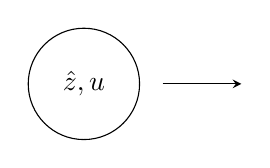
\begin{tikzpicture}
			\draw (4.707,0) arc [start angle=0, end angle=360, x radius=0.707, y radius=0.707];
			\node at(4,0.0){$\hat{z},u$};
			\draw[-stealth](5,0)--(6,0);
			\end{tikzpicture}}
	\end{figure}

	\noindent Usiamo chiaramente un simbolo analogo per una sorgente pura di stati down
		\begin{figure}[h!]
		\centering
		\scalebox{1}{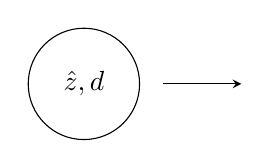
\begin{tikzpicture}
			\draw (4.707,0) arc [start angle=0, end angle=360, x radius=0.707, y radius=0.707];
			\node at(4,0.0){$\hat{z},d$};
			\draw[-stealth](5,0)--(6,0);
			\end{tikzpicture}}
	\end{figure}

	\noindent Chiediamoci ora cosa accade se consideriamo
	\begin{figure}[h!]
		\centering
		\scalebox{1}{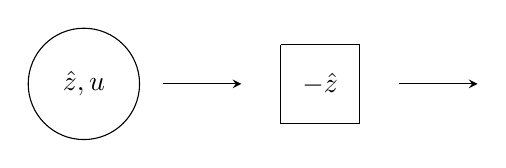
\begin{tikzpicture}
			\draw (-3+0.707,0) arc [start angle=0, end angle=360, x radius=0.707, y radius=0.707];
			\node at(-3,0.0){$\hat{z},u$};
			\draw[-stealth](-2,0)--(-1,0);
			\draw(-0.5,0.5)--(0.5,0.5)--(0.5,-0.5)--(-0.5,-0.5)--(-0.5,0.5);
			\node at(0,0.0){$-\hat{z}$};
			\draw[-stealth](1,0)--(2,0);
			\end{tikzpicture}}
	\end{figure}
	
	\newpage\noindent In tal caso il fascio che esce dall'apparato è tutto con spin down, nel senso che la deflessione di cui risente è verso $\hat{z}$. Questo è in accordo con l'idea di spin come grandezza vettoriale. Possiamo anche ripetere l'esperimento ruotando l'apparato di $90^\circ$, ossia usando un apparato con campo magnetico rivolto lungo $\hat{x}$. L'esito è analogo al primo esperimento descritto, ma questa volta indichiamo i due valori possibili dello spin con \textit{left} ($l$) e \textit{right} ($r$). Ovviamente
	\begin{figure}[h!]
		\centering
		\scalebox{1}{\begin{tikzpicture}
			\draw(-3,0.5)--(-2.5,0.5)--(-2.5,-0.5)--(-3,-0.5);		
			\draw[-stealth](-2,0)--(-1,0);
			\draw(-0.5,0.5)--(0.5,0.5)--(0.5,-0.5)--(-0.5,-0.5)--(-0.5,0.5);
			\node at(0,0.0){$\hat{x}$};
			\draw[-stealth](1,0)--(2,0);
			\node at(1.5,0)[above]{$l$};
			\node at(1.5,0)[below]{$r$};
			\end{tikzpicture}}
	\end{figure}

	\noindent Se invece consideriamo l'apparato
	\begin{figure}[h!]
		\centering
		\scalebox{1}{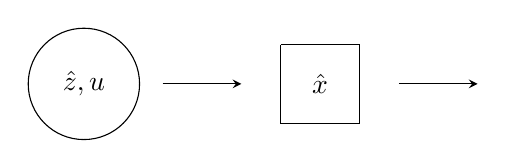
\begin{tikzpicture}
			\draw (-3+0.707,0) arc [start angle=0, end angle=360, x radius=0.707, y radius=0.707];
			\node at(-3,0.0){$\hat{z},u$};
			\draw[-stealth](-2,0)--(-1,0);
			\draw(-0.5,0.5)--(0.5,0.5)--(0.5,-0.5)--(-0.5,-0.5)--(-0.5,0.5);
			\node at(0,0.0){$\hat{x}$};
			\draw[-stealth](1,0)--(2,0);
			\end{tikzpicture}}
	\end{figure}
	
	\noindent si osserva ancora una divisione, sempre in parti uguali, del fascio tra atomi con spin left e atomi con spin right. Arrivati a questo punto, una spiegazione classica potrebbe ancora essere accettabile: per un qualche motivo strano, il valore di $\mu_z$ e di $\mu_x$ può solo essere $\pm1$, ma se accettiamo questo fatto l'apparato si comporta come un selettore per i valori di $\mu_z$ e di $\mu_x$. Se però incliniamo l'apparato in una direzione $\hat{n}=\cos\theta\hat{x}+\sin\theta\hat{z}$, si osserva ancora la divisione in due fasci. Questo \textit{non} è spiegabile se $\bm\mu$ si comporta come un vettore. Ancora peggio, possiamo immaginare un apparato formato da tre sottoapparati diretti lungo i versori $\hat{z}$, $\hat{e}_1=(\sqrt{3}/2)\hat{x}-(1/2)\hat{z}$ e $\hat{e}_2=-(\sqrt{3}/2)\hat{x}-(1/2)\hat{z}$. In tal modo, si ha
	\[\hat{z}+\hat{e}_1+\hat{e}_2=0\]
	e di conseguenza
	\[(\hat{z}+\hat{e}_1+\hat{e}_2)\cdot\bm\mu=0\]
	Questo risultato è privo di senso, perchè i valori possibili nella misura di $\hat{z}\cdot\bm\mu$, $\hat{e}_1\cdot\bm\mu$ e $\hat{e}_2\cdot\bm\mu$ sono $\pm1$, ma non possiamo ottenere 0 sommando un numero dispari di $\pm1$.\footnote{Questa incompatibilità tra le misure è essenzialmente dovuta al fatto che le matrici di Pauli
		\[
		\sigma_x=\left(\begin{array}{c c}
		0&1\\1&0
		\end{array}\right),\,\,\,\,\,\,\sigma_y=\left(\begin{array}{c c}
		0&-i\\i&0
		\end{array}\right),\,\,\,\,\,\,\sigma_z=\left(\begin{array}{c c}
		1&0\\0&-1
		\end{array}\right)
		\] non commutano tra di loro.} Consideriamo ora l'apparato\begin{figure}[h!]
		\centering
		\scalebox{1}{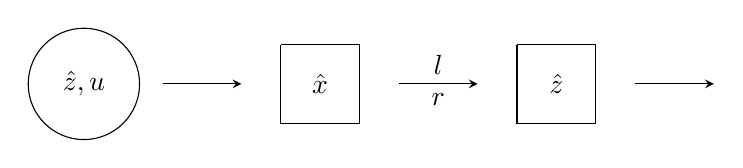
\begin{tikzpicture}
			\draw (-3+0.707,0) arc [start angle=0, end angle=360, x radius=0.707, y radius=0.707];
			\node at(-3,0.0){$\hat{z},u$};
			\draw[-stealth](-2,0)--(-1,0);
			\draw(-0.5,0.5)--(0.5,0.5)--(0.5,-0.5)--(-0.5,-0.5)--(-0.5,0.5);
			\node at(0,0.0){$\hat{x}$};
			\draw[-stealth](1,0)--(2,0);
			\node at(1.5,0)[above]{$l$};
			\node at(1.5,0)[below]{$r$};
			\draw(2.5,0.5)--(3.5,0.5)--(3.5,-0.5)--(2.5,-0.5)--(2.5,0.5);
			\node at(3,0.0){$\hat{z}$};
			\draw[-stealth](4,0)--(5,0);
			\end{tikzpicture}}
	\end{figure}

	\noindent Sperimentalmente si osserva che, all'uscita dell'apparato lungo $\hat{z}$, il fascio si divide nuovamente tra stato up e stato down. Questo controintuitivo risultato, unito a quello sugli apparati lungo $\hat{z}$ in cascata, mostra sperimentalmente come la misura di $\mu_x$ sia invasiva, nel senso che fa perdere l'informazione precedente su $\mu_z$. Come ultimo esempio, supponiamo di voler verificare tramite un esperimento di Stern-Gerlach la proposizione "$\mu_x=l\lor\mu_z=u$" per un fascio proveniente da una sorgente pura di stati up. Possiamo procedere in due modi distinti:
	\begin{enumerate}
		\item misuriamo $\mu_z$, \textit{poi} misuriamo $\mu_x$;
		\item misuriamo $\mu_x$, \textit{poi} misuriamo $\mu_z$.
	\end{enumerate}
	Classicamente non c'è alcuna distinzione tra i due procedimenti. D'altronde, come abbiamo visto, in meccanica classica le misure lasciano il sistema inalterato nel suo stato. Abbiamo ormai imparato che in meccanica quantistica ciò non è più vero: la prima procedura ci dice che la proposizione è vera nel 100\% dei casi, mentre la seconda solo nel 75\% dei casi.
	
	\noindent Notiamo incidentalmente che, a meno di deviare il fascio, possiamo misurare anche lo spin lungo $\hat{y}$. Nel seguito indichiamo con \textit{top} ($t$) e \textit{bottom} ($b$) i due stati possibili di $\mu_y$.
	\subsection{Assiomatizzazione parziale dell'apparato di Stern-Gerlach}
	Dobbiamo ora sviluppare un certo numero di assiomi che ci permettono di predire questi bizzarri comportamenti. Per prima cosa, postuliamo che lo stato proveniente da una sorgente pura sia associato a un vettore $\ket{\psi}$\footnote{Usiamo la notazione di Dirac, che sarà spiegata nella prossima sezione.} appartenente a un certo spazio di Hilbert $\H$, di dimensione opportuna. Ad esempio, per gli stati lungo i tre assi usiamo le notazioni $\ket{u},\ket{d},\ket{l},\ket{r},\ket{t}$ e $\ket{b}$. A questo punto postuliamo che $\ket{u}$ e $\ket{d}$ siano ortogonali, poichè esiste una misura in grado di distinguerli senza ambiguità, ossia
	\[\braket{u}{d}=0\]
	Inoltre, non ci sono altri gradi di libertà rilevanti. Imponiamo quindi $\dim\H=2$ e richiediamo che ogni altro stato $\ket{\psi}$ del sistema sia della forma
	\[\ket{\psi}=\alpha\ket{u}+\beta\ket{d}\]
	Come mostreremo tra poco, i coefficienti $\alpha,\beta$ sono generalmente complessi. Per lo spin left avremo allora
	\[\ket{l}=\alpha_l\ket{u}+\beta_l\ket{d}\]
	Postuliamo ora che $|\alpha_l|^2$ e $|\beta_l|^2$ siano le probabilità condizionate di misurare $l$, ossia
	\begin{align*}
	|\alpha_l|^2&=P(\mu_z=+1\vert\ket{l})\\
	|\beta_l|^2&=P(\mu_z=-1\vert\ket{l})
	\end{align*}
	Notiamo che per costruzione si ha $\alpha_l=\braket{u}{l}$ e $\beta_l=\braket{d}{l}$. Inoltre, sperimentalmente si osserva
	\[|\alpha_l|^2=|\beta_l|^2=\frac{1}{2}\]
	Ovviamente, questa condizione da sola non permette di determinare i due coefficienti. Possiamo però fare un discorso analogo per $\ket{r}$, ossia scrivere
	\[\ket{r}=\alpha_r\ket{u}+\beta_r\ket{d}\]
	con
	\[|\alpha_r|^2=|\beta_r|^2=\frac{1}{2}\]
	Inoltre, anche $\ket{l}$ e $\ket{r}$ devono essere ortogonali. Questo richiede
	\[\alpha^*_r\alpha_l+\beta^*_r\beta_l=0\]
	Tutte queste condizioni sono verificate se si pone
	\begin{align*}
		\ket{l}&=\frac{1}{\sqrt{2}}\left(\ket{u}+\ket{d}\right)\\
		\ket{r}&=\frac{1}{\sqrt{2}}\left(\ket{u}-\ket{d}\right)
	\end{align*}
	Ma, chiaramente, non è la scrittura più generale dei coefficienti: possiamo ad esempio moltiplicare $\alpha_l$ e $\beta_l$ per $e^{i\theta_l}$ e $\alpha_r$ e $\beta_r$ per $e^{i\theta_r}$, continuando a rispettare le condizioni date. Vedremo più avanti che in realtà queste fasi globali sono del tutto irrilevanti. Infine, possiamo ripetere il discorso anche per $\ket{t}$ e $\ket{b}$. In tal caso però abbiamo ulteriori condizioni, perchè potremmo scegliere anche $\left\{\ket{l},\ket{r}\right\}$ come base di $\H$. Queste considerazioni richiedono, a meno di fasi globali
	\begin{align*}
	\ket{t}&=\frac{1}{\sqrt{2}}\left(\ket{u}-i\ket{d}\right)\\
	\ket{b}&=\frac{1}{\sqrt{2}}\left(\ket{u}+i\ket{d}\right)
	\end{align*}	
	Quindi è essenziale che $\H$ sia complesso. Effettivamente, abbiamo costruito tre coppie di vettori mutuamente ortogonali tali che, comunque presi due vettori da coppie diverse, questi hanno sempre un angolo tra di loro di $\pi/4$. Questo è impossibile in uno spazio vettoriale reale a due dimensioni. Se però prendiamo $\H$ come spazio complesso, potrebbe sorgerci il dubbio che in realtà sia a quattro dimensioni, dato che due coefficienti complessi dipendono da quattro parametri reali. Non è così perchè uno dei parametri può essere eliminato togliendo le fasi globali, e un altro viene eliminato considerando la condizione di normalizzazione, necessaria per un'interpretazione probabilistica dei coefficienti. Questi due parametri hanno una sorta di analogo nel sistema reale: i due angoli necessari per determinare l'orientazione dell'apparato.
	\newpage
	\section{Assiomatizzazione della meccanica quantistica}
	\subsection{Richiami di analisi e geometria}
	Diamo per note le nozioni di spazio vettoriale, lineare indipendenza e base. Se non indicato, lo spazio si suppone su $\C$. Seguono alcune definizioni che dovrebbero essere già note, ma su cui, a volte, c'è ambiguità nella notazione usata dai matematici e dai fisici. Inoltre, daremo diversi risultati utili senza dimostrazione, dato che dovrebbero essere stati visti in altri corsi. Ci limiteremo a dimostrare solo alcuni ultimi teoremi e lemmi.
	\begin{definition}[Prodotto scalare] Sia $V$ uno spazio vettoriale. Un prodotto scalare su $V$ è una mappa $(,)\colon V\times V\to\C$ che gode di
		\begin{itemize}
			\item linearità nel secondo argomento,
			\item per ogni $v\in V$ si ha $(v,v)\geq0$, con uguaglianza se e solo se $v=0$,
			\item per ogni $v,w\in V$ si ha $(v,w)=(w,v)^*$.
		\end{itemize}
	\end{definition}
	\begin{lemma}[Disuguaglianza di Cauchy-Schwarz]
		Sia $V$ uno spazio vettoriale dotato di un prodotto scalare $(,)$. Allora per ogni $v,w\in V$
		\[\left|(v,w)\right|\leq\sqrt{(v,v)(w,w)}\]
	\end{lemma}
	\begin{definition}[Norma indotta]
		Sia $V$ uno spazio vettoriale dotato di un prodotto scalare $(,)$. La norma indotta dal prodotto scalare è la mappa $\norm{\cdot}\colon V\to\R$ definita da
		\[\norm{v}=\sqrt{(v,v)}\]
		e gode delle proprietà
		\begin{itemize}
			\item per ogni $v\in V$ si ha $\norm{v}\geq0$, con uguaglianza se e solo se $v=0$,
			\item per ogni $v\in V$ e $\lambda\in \C$ si ha $\norm {\lambda v}=|\lambda|\norm {v}$,
			\item vale la disuguaglianza triangolare, ovvero per ogni $v,w\in V$ si ha
			\[\norm {v+w}\leq\norm {v}+\norm{w}\]
		\end{itemize}
	\end{definition}
	\begin{definition}[Distanza indotta]
		Sia $V$ uno spazio vettoriale dotato di un prodotto scalare $(,)$. La distanza indotta dal prodotto scalare è
		la mappa $d\colon V\times V\to \R$ definita da
		\[d(v,w)=\norm {v-w}\]
		e gode delle proprietà
		\begin{itemize}
			\item per ogni $v,w\in V$ si ha $d(v,w)\geq0$, con uguaglianza se e solo se $v=w$,
			\item per ogni $v,w\in V$ si ha $d(v,w)=d(w,v)$,
			\item vale la disuguaglianza triangolare, ovvero per ogni $v,w,u\in V$ si ha
			\[d(v,w)\leq d(v,u)+d(u,w)\] 	
		\end{itemize}
	\end{definition}
	\begin{definition}[Successione di Cauchy]
		Siano $V$ uno spazio vettoriale con una norma $\norm {\cdot}$ e $\left\{v_n\right\}_{n\in \N}$ una successione in $V$. La successione è detta di Cauchy se per ogni $\varepsilon>0$ esiste $N_\varepsilon\in \N $ tale che per ogni $n,m\geq N_\varepsilon$ si ha
		\[\norm {v_n-v_m}<\varepsilon\]
	\end{definition}
	\begin{definition}[Spazio completo]
		Uno spazio vettoriale con una norma $\norm {\cdot}$ si dice completo o chiuso se tutte le successioni di Cauchy convergono.
	\end{definition}
	\begin{definition}[Spazio di Hilbert]
		Uno spazio di Hilbert $\H$ è uno spazio vettoriale dotato di prodotto scalare, completo rispetto alla norma indotta.	
	\end{definition}
	\subsubsection{Spazi a dimensione finita}
	D'ora in poi ci limitiamo al caso in cui $\dim \H<+\infty$, tratteremo poi il caso degli spazi a dimensione infinita.
	\begin{definition}[Funzionale e spazio duale]
		Sia $\H$ uno spazio di Hilbert. Un funzionale su $\H$ è una mappa lineare $\phi\colon \H \to\C $. L'insieme dei funzionali su $\H$ forma uno spazio vettoriale, detto spazio duale di $\H$ e indicato con $\H^\dagger$.
	\end{definition}
	\begin{theorem}[di rappresentazione di Riesz] Sia $f$ un funzionale su uno spazio di Hilbert $\H$. Allora esiste un unico vettore $w\in\H$ tale che per ogni $v\in V$
		\[f(v)=(w,v)\]
	\end{theorem}
	\begin{corollary}
		Uno spazio di Hilbert $\H$ è isomorfo al suo duale $\H^\dagger$.
	\end{corollary}
	\begin{definition}[Operatore]
		Un operatore su uno spazio di Hilbert $\H$ è un'applicazione lineare $\hat{\Theta}\colon\H \to\H$.
	\end{definition}
	Possiamo ora introdurre la notazione di Dirac: indichiamo i vettori di uno spazio di Hilbert $\H$ con la notazione $\ket{v}$. Il vettore così indicato è detto \textit{ket}. Inoltre, indichiamo gli elementi $\H^\dagger$ con la notazione $\bra{w}$, detto \textit{bra}. Dato l'isomorfismo tra $\H$ e $\H^\dagger$, indichiamo il prodotto scalare tra $\ket{v}$ e $\ket{w}$ con
	\[\braket{v}{w}\]
	Inoltre, indichiamo l'azione di un operatore $\hat{\Theta}$ su un vettore $\ket{v}$ con $\hat{\Theta}\ket{v}$. In tal modo, il prodotto scalare tra i vettori $\ket{v}$ e $\hat\Theta\ket{w}$ è
	\[\braketop{v}{\hat{\Theta}}{w}\]
	In particolare, il prodotto
	\[\braketop{v}{\hat{\Theta}}{v}\]
	è detto valore di aspettazione di $\hat{\Theta}$ sul vettore (o stato) $\ket{v}$. Infine, presi $\ket{v},\ket{w}\in\H$, possiamo definire il prodotto esterno $\hat{\Theta}=\ket{v}\bra{w}$. Questo operatore agisce su $\ket{u}\in\H$ con
	\[\hat{\Theta}\ket{u}=\braket{w}{u}\ket{v}\]
	Si noti che
	\[\mathrm{tr}(\ket{v}\bra{w})=\braket{w}{v}\]
	Se $\ket{v}$ ha norma 1, allora $\hat\Pi=\ket{v}\bra{v}$ è il proiettore su $\ket{v}$.
	\begin{definition}[Matrice associata a un operatore]
		Siano $\hat{\Theta}$ un operatore su uno spazio di Hilbert $\H$ di dimensione $d$ e $\left\{\ket{e_i}\right\}_{i=1}^{d}$ una base di $\H$. La matrice $M$ associata a $\hat{\Theta}$ nella base scelta è la matrice con coefficienti
		\[M_{ij}=\braketop{e_i}{\hat{\Theta}}{e_j}\]
	\end{definition}
	\begin{lemma}
		Nelle ipotesi precedenti, se indichiamo con $\alpha_{\ket{v}},\alpha_{\hat{\Theta}\ket{v}}\in \C ^d$ le $d$-uple delle coordinate di $\ket{v
		}$ e $\hat{\Theta} \ket {v}$ rispetto alla base fissata, si ha
		\[\alpha_{\hat{\Theta}\ket{v}}=M\alpha_{\ket{v}}\] 
	\end{lemma}
	\begin{definition}[Prodotto di operatori, commutatore e anticommutatore]
		Siano $\hat{\Theta}_1,\hat{\Theta}_2$ due operatori su uno spazio di Hilbert $\H$. Il loro prodotto $\hat{\Theta}_1\hat{\Theta}_2$ è definito come la loro composizione ed è, in generale, non commutativo. Il commutatore tra $\hat{\Theta}_1$ e $\hat{\Theta}_2$ è
		\[[\hat{\Theta}_1,\hat{\Theta}_2]=\hat{\Theta}_1\hat{\Theta}_2-\hat{\Theta}_2\hat{\Theta}_1\]
		mentre l'anticommutatore è
		\[\{\hat{\Theta}_1,\hat{\Theta}_2\}=\hat{\Theta}_1\hat{\Theta}_2+\hat{\Theta}_2\hat{\Theta}_1\]
		Diremo che i due operatori (anti)commutano o sono (anti)commutanti se il loro (anti)commutatore è l'operatore nullo.
	\end{definition}
	\begin{definition}[Operatore aggiunto]
		Sia $\hat{\Theta}$ un operatore su uno spazio di Hilbert $\H$. L'operatore aggiunto $\hat{\Theta}^\dagger$ è definito come l'operatore tale che per ogni $\ket{v},\ket{w}\in\H$ si abbia
		\[\braketop{w}{\hat{\Theta}^\dagger}{v}=\left(\braketop{v}{\hat{\Theta}}{w}\right)^*\]
	\end{definition}
	Si noti che se $M$ è la matrice associata a $\hat{\Theta}$ in una data base, allora $M^\dagger$ è la matrice associata a $\hat{\Theta}^\dagger$ nella stessa base. Inoltre, senza la notazione di Dirac la definizione di aggiunto è in un certo senso più semplice: è l'operatore tale che, per ogni $v,w\in \H$, si abbia
	\[(\hat{\Theta}^\dagger v,w)=(v,\hat{\Theta}w)\]
	\begin{definition}[Operatore normale]
		Un operatore $\hat{\Theta}$ su uno spazio di Hilbert $\H$ si dice normale se $[\hat{\Theta},\hat{\Theta}^\dagger]=0$.		
	\end{definition}
		\begin{definition}[Operatore isometrico]
		Un operatore $\hat{\Theta}$ su uno spazio di Hilbert $\H$ si dice isometrico se $\hat{\Theta}^\dagger\hat{\Theta}=\id_\H$.		
	\end{definition}
	\begin{definition}[Operatore unitario]
	Un operatore $\hat{\Theta}$ su uno spazio di Hilbert $\H$ si dice unitario se è normale e isometrico.		
\end{definition}
	\begin{definition}[Operatore hermitiano]
	Un operatore $\hat{\Theta}$ su uno spazio di Hilbert $\H$ si dice hermitiano (o autoaggiunto) se $\hat{\Theta}=\hat{\Theta}^\dagger$.		
\end{definition}
	\begin{definition}[Operatore positivo]
	Un operatore $\hat{\Theta}$ su uno spazio di Hilbert $\H$ si dice positivo, e si scrive $\hat{\Theta}\geq0$, se il suo valore di aspettazione è non negativo su ogni stato, ossia se per ogni $\ket{\psi}\in\H$ si ha $\braketop{\psi}{\hat{\Theta}}{\psi}\geq0$.
\end{definition}
Si noti che un operatore positivo è necessariamente autoaggiunto e che un operatore autoaggiunto è necessariamente normale. Inoltre, un operatore isometrico è necessariamente normale.
\begin{definition}[Autovettori e autovalori]
	Sia $\hat{\Theta}$ un operatore su uno spazio di Hilbert $\H$. $\ket{v}\in\H\backslash\{0\}$ si dice autovettore di $\hat{\Theta}$ relativo all'autovalore $\lambda\in\C$ se
	\[\hat{\Theta}\ket{v}=\lambda\ket{v}\]
\end{definition}
\begin{definition}
	Siano $\lambda\in\C$, $\hat{\Theta}$ un operatore su uno spazio di Hilbert $\H$. Il polinomio caratteristico $p_{\hat{\Theta}}$ di $\hat{\Theta}$ è il polinomio
	\[p_{\hat{\Theta}}(\lambda)=\det(\hat{\Theta}-\lambda\id)\]
\end{definition}
\begin{theorem}
	Gli autovalori di $\hat{\Theta}$ sono tutte e sole le radici di $p_{\hat{\Theta}}$.
\end{theorem}
\begin{lemma}
	Gli autovalori di un operatore autoaggiunto sono reali.
\end{lemma}
\begin{lemma}
	Gli autovalori di un operatore isometrico hanno modulo 1.
\end{lemma}
\begin{lemma}
	Gli autovettori di un operatore normale relativi ad autovalori distinti sono ortogonali.
\end{lemma}
\begin{lemma}
	Se $\lambda\in\ C$ è un autovalore per un operatore normale $\hat{\Theta}$ e $\ket{v}$ è un autovettore relativo a $\lambda$, allora $\ket{v}$ è un autovettore anche per $\hat{\Theta}^\dagger$ con autovalore $\lambda^*$.
\end{lemma}
\begin{theorem}\label{commuta}
	Siano $\hat{A},\hat{B}$ due operatori diagonalizzabili su uno spazio di Hilbert $\H$. Allora esiste una base di $\H$ di autovettori per $\hat{A}$ e $\hat{B}$ se e solo se $[\hat{A},\hat{B}]=0$.
\end{theorem}
\begin{theorem}[Teorema spettrale per operatori autoaggiunti]
	Sia $\hat{\Theta}$ un operatore autoaggiunto su uno spazio di Hilbert $\H$. Allora esiste una base ortonormale di $\H$ di autovettori di $\hat{\Theta}$.
\end{theorem}
\begin{proof}
	Procediamo per induzione su $d=\dim\H$. Per $d=1$ non c'è nulla da mostrare. Supponiamo ora $d>1$ e sia $\lambda_1$ un autovalore di $\hat{\Theta}$, con autovettore $\ket{e_1}$ normalizzato. Completiamo $\ket{e_1}$ a base $\left\{\ket{e_1},\ket{v_2},\dots,\ket{v_d}\right\}$ di $\H$ in modo che $\ket{e_1}$ sia ortogonale a tutti gli altri vettori di base. In tal modo, se $M$ è la matrice associata a $\hat{\Theta}$ in tale base si ha
	\[M_{i1}=\braketop{e_i}{\hat{\Theta}}{e_1}=\lambda_1\delta_{i1}\]
	In particolare, $M_{i1}=0$ per $i\geq2$. Dato che l'operatore è autoaggiunto, allora $M_{ij}=M_{ji}^*$, dunque $M_{1i}=0$ per $i\geq2$. Quindi se $W\subseteq\H$ è il sottospazio generato da $\ket{v_2},\dots,\ket{v_d}$ si ha $\hat{\Theta}(W)\subseteq W$, inoltre $\dim W=d-1$, quindi per ipotesi induttiva esiste una base ortonormale $\mathcal{B}$ di $W$ di autovettori per $\hat{\Theta}|_{W}$. Chiaramente $\mathcal{B}\cup\left\{\ket{e_1}\right\}$ è una base ortonormale di $\H$ di autovettori di $\hat{\Theta}$.
\end{proof}
\begin{lemma}
	Sia $\hat{\Theta}$ un operatore su uno spazio di Hilbert $\H$. $\hat{\Theta}$ è normale se e solo se esistono due operatori $\hat{A},\hat{B}$ autoaggiunti e commutanti tali $\hat{\Theta}=\hat{A}+i\hat{B}$.
\end{lemma}
\begin{proof}
	La freccia $\Leftarrow$ è ovvia. Per l'altra freccia, definiamo
	\begin{align*}
		\hat{A}&=\frac{\hat{\Theta}+\hat{\Theta}^\dagger}{2}\\
		\hat{B}&=\frac{\hat{\Theta}-\hat{\Theta}^\dagger}{2i}
	\end{align*}
	Chiaramente $\hat{A}$ e $\hat{B}$ sono due operatori autoaggiunti tali che $\hat{\Theta}=\hat{A}+i\hat{B}$. Inoltre
	\begin{align*}
		[\hat{A},\hat{B}]&=\frac{(\hat{\Theta}+\hat{\Theta}^\dagger)(\hat{\Theta}-\hat{\Theta}^\dagger)}{4i}-\frac{(\hat{\Theta}-\hat{\Theta}^\dagger)(\hat{\Theta}+\hat{\Theta}^\dagger)}{4i}=\\&=0
	\end{align*}
\end{proof}
\begin{theorem}[Teorema spettrale]
	Sia $\hat{\Theta}$ un operatore su uno spazio di Hilbert $\H$. Allora $\hat{\Theta}$ è normale se e solo se esiste una base ortonormale di $\H$ di autovettori di $\hat{\Theta}$.
\end{theorem}
\begin{proof}
	Di nuovo, la freccia $\Leftarrow$ è banale. Per l'altra freccia, basta usare la decomposizione data dal lemma precedente e il teorema \ref{commuta} per concludere.
\end{proof}
\begin{definition}[Prodotto tensoriale di spazi vettoriali]
	Siano $V$, $W$ due spazi vettoriali. Un prodotto di tensoriale di $V$ e $W$, indicato con $V\widehat{\otimes} W$, è uno spazio vettoriale dotato di una mappa bilineare $\widehat\otimes\colon V\times W\to V\widehat\otimes W$, che associa la coppia $(v,w)\in V\times W$ all'elemento $v\widehat\otimes w\in V\widehat\otimes W$, tale che, preso uno spazio vettoriale $Z$ qualunque, per ogni mappa bilineare $h\colon V\times W\to Z$ esiste una mappa lineare $h'\colon V\widehat\otimes W\to Z$ che faccia commutare il diagramma
	\[\begin{tikzcd}
	V\times W \arrow[dr, "h"] \arrow[r, "\widehat{\otimes}"]&V\widehat{\otimes} W\arrow[d, "h'"]\\
	&Z
	\end{tikzcd}\]
\end{definition}
\begin{theorem}\label{tensorbase}
	Il prodotto tensoriale $V\widehat{\otimes}W$ esiste ed è unico a meno di isomorfismi. Inoltre, se $\left\{v_i\right\}_{i\in I}$ e $\left\{w_j\right\}_{j\in J}$ sono rispettivamente una base di $V$ e una base di $W$, allora $\left\{v_i\widehat{\otimes}w_j\right\}_{(i,j)\in I\times J}$ è una base di $V\widehat{\otimes}W$.
\end{theorem}
\begin{definition}
	I vettori di $V\widehat{\otimes}W$ della forma $v\widehat{\otimes}w$, con $v\in V$ e $w\in W$, sono detti vettori decomponibili.
\end{definition}
\begin{definition}[Prodotto tensoriale di spazi di Hilbert] Siano $\H$, $\H'$ due spazi di Hilbert con prodotti scalari $(,)_\H$ e $(,)_{\H'}$. Definiamo sui vettori decomponibili di $\H\widehat{\otimes}\H'$ il prodotto scalare $\left(,\right)\colon(\H\widehat{\otimes}\H')\times(\H\widehat{\otimes}\H')\to\C$
	\[(v_1\widehat{\otimes}v_1',v_2\widehat{\otimes}v_2')=(v_1,v_2)_\H(v_1',v_2')_{\H'}\]
Il prodotto tensoriale di $\H$ e $\H'$, indicato con $\H\otimes\H'$, è il completamento metrico di $\H\widehat{\otimes}\H'$.
\end{definition}

Nel seguito, useremo il prodotto tensoriale di spazi di Hilbert per studiare un sistema composito a partire dai suoi sottosistemi. Indicheremo con stati entangled gli stati indecomponibili, e questi avranno un ruolo importante dal punto di vista interpretativo: rappresenteranno infatti degli stati che non hanno un analogo classico. In ogni caso si noti che, per il teorema \ref{tensorbase}, comunque preso $\ket{\psi}\in\H\otimes\H'$ esistono due successioni $\left\{\ket{\phi_n}_\H\right\}_{n\in\N}\subseteq\H$ e $\left\{\ket{\chi_m}_{\H'}\right\}_{m\in \N}\subseteq\H'$ tali che 
\[\ket{\psi}=\sum_{k}\ket{\phi_k}_\H\otimes\ket{\chi_k}_{\H'}\]
Viceversa, gli stati decomponibili saranno chiamati indifferentemente stati prodotto, stati fattorizzati o stati non entangled. Inoltre, per il prodotto tensoriale useremo, quando non ambigue, le notazioni \[\ket{\psi}_{\H}\otimes\ket{\phi}_{\H'}=\ket{\psi}\otimes\ket{\phi}=\ket{\psi}_\H\ket{\phi}_{\H'}=\ket{\psi,\phi}_{\H,\H'}=\ket{\phi}_{\H'}\otimes\ket{\psi}_\H=\ket{\phi}_\H\ket{\psi}_{\H'}\]
In particolare, utilizzando le ultime due notazioni indicheremo sempre con un pedice lo spazio a cui appartengono i ket.
\begin{definition}[Prodotto tensoriale di operatori]
	Siano $\hat{\Theta}_{\H}$ e $\hat{\Omega}_{\H'}$ due operatori, rispettivamente sugli spazi di Hilbert $\H$ e $\H'$. Il prodotto tensoriale dei due operatori è l'operatore $\hat{\Theta}_\H\otimes\hat{\Omega}_{\H'}$ su $\H\otimes\H'$ definito sugli stati non entangled da
	\[\hat{\Theta}_\H\otimes\hat{\Omega}_{\H'}(\ket{\psi}_\H\otimes\ket{\phi}_{\H'})=(\hat{\Theta}_\H\ket{\psi}_\H)\otimes(\hat{\Omega}_{\H'}\ket{\phi}_{\H'})\]
\end{definition}
Se uno dei due operatori (ad esempio $\hat{\Omega}_\H'$) è l'identità, spesso indicheremo per brevità $\hat{\Theta}_\H\otimes\id_{\H'}$ direttamente con $\hat{\Theta}_\H$.
Inoltre, in maniera analoga a quanto visto con gli stati, se $\hat{\Lambda}$ è un operatore su $\H\otimes\H'$ allora esistono due successioni di operatori $\left\{\hat{\Theta}_{\H}^{(n)}\right\}_{n\in \N}$ e $\left\{\hat{\Omega}_{\H'}^{(m)}\right\}_{m\in \N}$, rispettivamente su $\H$ e $\H'$, tali che
\[\hat{\Lambda}=\sum_{k}\hat{\Theta}_{\H}^{(k)}\otimes\hat{\Omega}_{\H'}^{(k)}\]
Gli operatori "decomponibili", cioè scrivibili come prodotto di due operatori sui due spazi, saranno chiamati operatori locali.
\begin{definition}[Contrazione]
	Presi due spazi di Hilbert $\H$ e $\H'$, e presi $\ket{\chi}_{\H}\in\H$ e $\ket{\psi}_{\H\otimes\H'}\in \H\otimes\H'$, la contrazione tra i due vettori è 
	\[\tensor*[_{\H}]{\bra{\chi}}{}\psi\rangle_{\H\otimes\H'}\]
\end{definition}
Si noti che la contrazione è un vettore di $\H'$. Infatti, fissate due basi ortonormali $\left\{\ket{i}_\H\right\}_{i\in I}$ e $\left\{\ket{j}_{\H'}\right\}_{j\in J}$ di $\H$ e $\H'$, si ha
\begin{align*}
	\ket{\chi}_\H&=\sum_{i\in I}\alpha_{i}\ket{i}_\H\\
	\ket{\psi}_{\H\otimes\H'}&=\sum_{(i,j)\in I\times J}\beta_{ij}\ket{i}_\H\otimes\ket{j}_{\H'}
\end{align*}
e quindi
\[\tensor*[_{\H}]{\bra{\chi}}{}\psi\rangle_{\H\otimes\H'}=\sum_{(i,j)\in I\times J}\alpha_i^*\beta_{ij}\ket{j}_{\H'}\in \H'\]

\noindent Ovviamente, le definizioni date finora si estendono anche al prodotto tensoriale di più spazi di Hilbert.
\subsubsection{Spazi a dimensione infinita}
In questa sezione non usiamo la notazione di Dirac. Molti dei risultati appena visti non valgono nel caso generale: saremo quindi interessati a dare opportune restrizioni per avere risultati simili al caso finito dimensionale.
\begin{definition}[Convergenza forte e debole]
	Sia $\left\{e_n\right\}_{n\in\N}$ una successione in uno spazio di Hilbert $\H$. Si dice che la successione converge fortemente (o in norma) a $e\in\H$ se
	\[\lim\limits_{n\to+\infty}\norm{e_n-e}=0\]
	Si dice che la successione converge debolmente a $e\in\H$ se per ogni $v\in\H$ si ha
	\[\lim\limits_{n\to+\infty}(v,e_n)=(v,e)\]
\end{definition}
\begin{lemma}
	La convergenza forte implica la convergenza debole.
\end{lemma}
\begin{lemma}[Disuguaglianza di Bessel] Siano $\H$ uno spazio di Hilbert a dimensione infinita, $\left\{v_k\right\}_{k\in\N}\subseteq\H$ una successione di vettori ortonormali e $\left\{\alpha_k\right\}_{k\in \N}\subseteq\C$ una successione di complessi. Allora, per ogni $w\in\H$ e per ogni $N\in \N$, la grandezza
	\[\norm{w-\sum_{j=0}^{N}\alpha_jv_j}\]
è minima per $\alpha_j=(v_j,w)$. Inoltre, si ha
\[\sum_{j=0}^{N}|(v_j,w)|^2\leq\norm {w}^2\]
\end{lemma}
\begin{proof}
	Si ha 
	\begin{align*}
	0&\leq\norm{w-\sum_{j=0}^{N}\alpha_jv_j}^2=\\&=\norm {w}^2+\sum_{j=0}^{N}|\alpha_j|^2-2\Re\sum_{j=0}^{N}\alpha_j(w,v_j)=\\&=\norm {w}^2-\sum_{j=0}^{N}|(v_j,w)|^2+\sum_{j=1}^{N}|\alpha_j-(v_j,w)|^2
	\end{align*}
	Quindi la norma iniziale è minima se $\alpha_j=(v_j,w)$. Inoltre, in tal caso segue la disuguaglianza di Bessel.
\end{proof}
\begin{lemma}
	Siano $\H$ uno spazio di Hilbert, $\left\{v_k\right\}_{k\in \N}\subseteq\H$ una successione di vettori ortonormali, $w\in \H$. La successione
	\[w_n=\sum_{k=0}^{n}(v_k,w)v_k\]
	è di Cauchy.
\end{lemma}
\begin{definition}[Insieme ortonormale completo]
	Nelle ipotesi del lemma precedente, se per ogni $w\in\H$ si ha $w=\lim\limits_{n\to+\infty}w_n$, la successione $\left\{v_k\right\}_{k\in \N}$ forma un insieme ortonormale completo.
\end{definition}
\begin{definition}[Spazio di Hilbert separabile]
	Uno spazio di Hilbert $\H$ è separabile se ha un sottoinsieme numerabile e denso.
\end{definition}
\begin{theorem}
	Uno spazio di Hilbert $\H$ è separabile se e solo se ammette un insieme ortonormale completo numerabile.
\end{theorem}
\begin{theorem}
	Lo spazio
	\[l_2=\left\{a=\left\{a_n\right\}_{n\in\N}\subseteq \C:\sum_{n=0}^{+\infty}|a_n|^2<+\infty\right\}\]
	munito del prodotto scalare
	\[(a,b)=\sum_{n=0}^{+\infty}a_n^*b_n\]
	è uno spazio di Hilbert separabile.
\end{theorem}
\begin{theorem}
	Ogni spazio di Hilbert $\H$ separabile è isomorfo a $l_2$.
\end{theorem}
\begin{theorem}
	Lo spazio
	\[\L ^2(\R)=\left\{f\colon\R \to\C :\int_{-\infty}^{+\infty}|f(x)|^2\d x<+\infty\right\}\]
	munito del prodotto scalare
	\[(f,g)=\int_{-\infty}^{+\infty}f^*(x)g(x)\d x\]
	e a meno della relazione di equivalenza $f\sim g$ se $f=g$ quasi ovunque, è uno spazio di Hilbert.
\end{theorem}
Consideriamo ora lo spazio degli operatori lineari su $\H$: lo indicheremo con $\mathcal{L}(\H)$. Dato che lavoriamo in uno spazio a dimensione infinita, si possono anche considerare operatori non definiti su tutto lo spazio\footnote{A differenza del caso finito dimensionale, definire un operatore su un insieme ortonormale completo \textit{non} significa definirlo su tutto lo spazio.}: se $\hat{\Theta}$ è un operatore, indichiamo il suo dominio con $\mathcal{D}(\hat{\Theta})$.
\begin{definition}[Norma operatoriale]
	Sia $\hat{\Theta}\in\mathcal{L}(\H)$. La norma di $\hat{\Theta}$ è
	\[\Vert \hat{\Theta}\Vert=\sup_{v\in \H\backslash\{0\}}\frac{\Vert {\hat{\Theta}v}\Vert}{\norm {v}}\]
\end{definition}
\begin{definition}[Operatore limitato]
	Sia $\hat{\Theta}\in\mathcal{L}(\H)$. Se $\Vert{\hat{\Theta}}\Vert<+\infty$, diciamo che $\hat{\Theta}$ è limitato. Lo spazio degli operatori limitati è $\mathcal{B}(\H)$.
\end{definition}
\begin{definition}[Operatore chiuso]
	Sia $\hat{\Theta}$ un operatore lineare in uno spazio di Hilbert $\H$ con dominio $\mathcal{D}(\hat{\Theta})$. $\hat{\Theta}$ si dice chiuso se per ogni successione $\left\{v_n\right\}_{n\in\N}\subseteq\mathcal{D}(\hat{\Theta})$ tale che esistano $v=\lim\limits_{n\to+\infty}v_n$ e $w=\lim\limits_{n\to+\infty}\hat{\Theta}v_n$, si ha $v\in\mathcal{D}(\hat{\Theta})$ e $w=Tv$. 
\end{definition}
\begin{definition}[Operatore aggiunto]
	Sia $\hat{\Theta}$ un operatore con dominio $\mathcal{D}(\hat{\Theta})$ denso in $\H$. Sia
	\[\mathcal{A}=\left\{v\in\H:\textrm{ esiste }\overline{v}\in\H\textrm{ tale che per ogni }w\in\mathcal{D}(\hat{\Theta}),\,(v,\hat{\Theta}w)=(\overline{v},w)\right\}\]
	L'operatore aggiunto $\hat{\Theta}^\dagger$ di $\hat{\Theta}$ è l'operatore con dominio $\mathcal{D}(\hat{\Theta}^\dagger)=\mathcal{A}$ tale che per ogni $w\in\mathcal{D}(\hat{\Theta})$ e per ogni $v\in\mathcal{D}(\hat{\Theta}^\dagger)$
	\[(\hat{\Theta}^\dagger v,w)=(v,\hat{\Theta}w)\]
\end{definition}
Si noti che la densità del dominio è essenziale per definire l'aggiunto. Infatti, se esistono due vettori $v_1,v_2\in\H$ tali che per ogni $w\in\mathcal{D}(\hat{\Theta})$ si abbia
\[(v_1-v_2,w)=0\]
allora, grazie alla densità di $\mathcal{D}(\hat{\Theta})$ e alla continuità del prodotto scalare si ha la stessa uguaglianza per ogni $w\in\H$, e quindi $v_1=v_2$.
\begin{definition}[Operatore hermitiano]
	Un operatore $\hat{\Theta}$ si dice hermitiano se per ogni $v,w\in\mathcal{D}(\hat{\Theta})$ si ha
	\[(w,\hat{\Theta}v)=(\hat{\Theta}w,v)\]
\end{definition}
Si noti che un operatore hermitiano non coincide in generale con il suo aggiunto, dato che questo potrebbe non esistere o avere un dominio diverso.
\begin{definition}[Operatore simmetrico]
	Un operatore $\hat{\Theta}$ è simmetrico se è hermitiano e $\mathcal{D}(\hat{\Theta})$ è denso in $\H$.
\end{definition}
\begin{definition}[Operatore autoaggiunto]
	Un operatore $\hat{\Theta}$ è autoaggiunto se è simmetrico e se $\mathcal{D}(\hat{\Theta})=\mathcal{D}(\hat{\Theta}^\dagger)$.
\end{definition}
\begin{definition}[Operatore compatto]
	Un operatore $\hat{\Theta}$ si dice compatto se per ogni successione limitata $\left\{v_n\right\}_{n\in\N}\subseteq\mathcal{D}(\hat{\Theta})$ esiste una sottosuccessione $\left\{v_{n_j}\right\}_{j\in\N}$ tale che la successione $\left\{\hat{\Theta}v_{n_j}\right\}_{j\in\N}$ converge in modo forte. Lo spazio degli operatori compatti sarà indicato con $\mathcal{B}_\infty(\H)$.
\end{definition}
\begin{lemma}
	Un operatore compatto è limitato.
\end{lemma}
\begin{lemma}
	Un operatore è compatto se e solo se la chiusura dell'immagine di un qualunque sottoinsieme limitato del dominio è compatta.
\end{lemma}
Si noti che la proprietà di compattezza è molto forte: ad esempio, l'identità non è compatta.
\begin{definition}[Operatore di classe traccia]
	Un operatore $\hat{\Theta}$ è di classe traccia se esiste un sistema ortonormale completo $\left\{e_i\right\}_{i\in\N}$ tale che
	\[\sum_{i=0}^{+\infty}(e_i,\sqrt{\hat{\Theta}^\dagger\hat{\Theta}}\,e_i)<+\infty\]
	Lo spazio degli operatori di classe traccia sarà indicato con $\mathcal{B}_1(\H)$.
\end{definition}
Gli operatori di classe traccia sono particolarmente importanti perchè, come vedremo, a un dato sistema fisico sarà possibile associare un operatore, detto matrice densità, che è di questo tipo. Inoltre, se $\hat{\Theta}\in\mathcal{B}_1(\H)$, è possibile definire come in dimensione finita la traccia $\tr\hat{\Theta}$.
\begin{theorem}[Teorema spettrale compatto autoaggiunto]
	Sia $\hat{\Theta}$ un operatore compatto e autoaggiunto con dominio $\H$. Allora vale uno dei seguenti enunciati:
	\begin{itemize}
		\item $\hat{\Theta}$ ha un numero finito di autovalori $\lambda_1,\dots,\lambda_n$ non nulli. Detto $\H_j$ l'autospazio relativo a $\lambda_j$, si ha $\dim\H_j<+\infty$ per ogni $j=1,\dots,n$. Inoltre, vale la decomposizione
		\[\H=\ker\hat{\Theta}\oplus \H_1\oplus\dots\oplus\H_n\]
		ed esiste una base ortonormale $\{e^j_i\}_{1\leq i\leq \dim\H_j,1\leq j\leq n}$ di autovettori di $(\ker \hat{\Theta})^\perp$ di $\hat{\Theta}$. Si ha infine per ogni $v\in\H$
		\[\hat{\Theta}v=\sum_{j=1}^{n}\lambda_j\sum_{i=1}^{\dim\H_j}(e^j_i,v)e^j_i\]
		\item $\hat{\Theta}$ ha un'infinità numerabile di autovalori non nulli $\lambda_i$, $i\in\N$, ordinabili in modo che
		\[\lim\limits_{n\to+\infty}\lambda_n=0\]
		Detto $\H_j$ l'autospazio relativo a $\lambda_j$, si ha $\dim\H_j<+\infty$ per ogni $j\in\N$. Inoltre, vale la decomposizione
		\[\H=\ker\hat{\Theta}\oplus\bigoplus_{j=0}^{+\infty}\H_j\]
		ed esiste una base ortonormale $\{e^j_i\}_{1\leq i\leq \dim\H_j,j\in\N}$ di $(\ker \hat{\Theta})^\perp$ di autovettori di $\hat{\Theta}$. Si ha infine per ogni $v\in\H$
		\[\hat{\Theta}v=\sum_{j=0}^{+\infty}\lambda_j\sum_{i=1}^{\dim\H_j}(e^j_i,v)e^j_i\]
	\end{itemize}
\end{theorem}


Limitarsi però ai soli operatori compatti autoaggiunti sarebbe un limite notevole per lo sviluppo della teoria. Cerchiamo adesso di adattare alcune definizioni per avere una trattazione decente dello spettro di un operatore.
\begin{definition}[Autovalore generalizzato]
	Siano $\hat{\Theta}$ un operatore in uno spazio di Hilbert $\H$ e $\lambda\in\C$. $\lambda$ è un autovalore generalizzato per $\hat{\Theta}$ se esiste una successione $\left\{v^{(n)}_\lambda\right\}_{n\in\N}\subseteq\mathcal{D}(\hat{\Theta})$ di vettori normalizzati tali che
	\[\lim\limits_{n\to+\infty}\Vert\hat{\Theta}v^{(n)}_\lambda-\lambda v^{(n)}_\lambda\Vert=0\] 
\end{definition}
\begin{theorem}[Weyl]
	$\lambda$ è un autovalore generalizzato per $\hat{\Theta}$ se e solo se $\hat{\Theta}-\lambda\id$ non è invertibile.
\end{theorem}
Si noti che in dimensione finita non c'è distinzione tra autovalori e autovalori generalizzati. Vediamo ora un esempio: consideriamo l'operatore $\hat{Q}\colon\mathcal{D}(\hat{Q})\to\mathbb{L}^2(\mathbb{R})$ definito da
\[\pos[f](x)=xf(x)\]
Il dominio è evidentemente
\[\mathcal{D}(\pos)=\left\{f\in\L^2(\R):xf(x)\in\L^2(\R)\right\}\]
Si può mostrare che un tale dominio è denso in $\L^2(\R)$, dunque possiamo considerare l'aggiunto $\pos^\dagger$. Si mostra facilmente che $\pos^\dagger=\pos$ e $\mathcal{D}(\pos^\dagger)=\mathcal{D}(\pos)$, quindi $\pos$ è autoaggiunto. Se $f_\lambda$ è un autofunzione relativa a $\lambda$ (che supponiamo reale), si deve avere
\[(\lambda-x)f_\lambda(x)=0\]
Quindi $f_\lambda$ ha come supporto $\left\{\lambda\right\}$, ossia $f_\lambda=0$, dunque $\pos$ non ha autovalori propri. Si definisca ora la successione
\[f^{(n)}_\lambda(x)=\sqrt{\frac{n}{2}}\chi_{A_{\lambda,n}}(x)\]
dove $\chi_{A_{\lambda,n}}$ è la funzione caratteristica dell'intervallo
\[A_{\lambda,n}=\left[\lambda-\frac{1}{n},\lambda+\frac{1}{n}\right]\]
Allora banalmente $\Vert f^{(n)}_\lambda\Vert=1$ per ogni $n$ e inoltre
\[\lim\limits_{n\to+\infty}\norm{\pos f^{(n)}_\lambda-\lambda f^{(n)}_{\lambda}}=0\]
Quindi lo spettro di $\pos$ è tutto l'asse reale, nonostante non esistano autovettori. Si può però pensare di estendere in qualche modo $\L^2(\R)$ in modo che abbia più "funzioni". Ad esempio, se consideriamo l'equazione agli autovalori per $\pos$ nel senso delle distribuzioni, la soluzione è semplicemente
\[f_\lambda(x)=A\delta(x-\lambda)\]
In tal senso, possiamo pensare alla $\delta$ come a un autovettore generalizzato.
\begin{definition}[Tripla di Gelfand]
	Una tripla di Gelfand è una tripla $(\Phi,\H,\Phi^\dagger)$, dove $\H$ è uno spazio di Hilbert, $\Phi$ un sottospazio denso di $\H$ che abbia una struttura di spazio vettoriale topologico tale che l'inclusione $\iota\colon\Phi\to\H$ sia continua. 
\end{definition}
Grazie al teorema di rappresentazione di Riesz, possiamo identificare $\H$ come sottospazio di $\Phi^\dagger$, e considerare quest'ultimo come una sorta di allargamento di $\H$. Nell'esempio precedente potremmo considerare la tripla di Gelfand $(\mathcal{S},\L^2(\R),\mathcal{S}^\dagger)$, dove $\mathcal{S}$ è la classe di Scwhartz e $\mathcal{S}^\dagger$ è lo spazio delle distribuzioni temperate. Riprendiamo adesso la notazione di Dirac, in cui i risultati che seguono si possono esprimere in maniera più semplice. In particolare, identifichiamo $f\in\L^2(\R)$ con $\ket{f}$ e la delta di Dirac centrata in $x_0$ con $\ket{x_0}$, la valutazione di $f$ in $x_0$ con $\braket{x_0}{f}$. Dal fatto che
\[f(x)=\int \d y f(y)\delta(x-y)\]
segue che l'identità si scrive nella forma
\[\id=\int \d x\ket{x}\bra{x} \]
mentre l'operatore $\pos$ dell'esempio precedente, che ha come autovalore generalizzato $x$ e come autovettore generalizzato $\ket{x}$, si scrive come
\[\pos=\int \d x\, x\ket{x}\bra{x}\]
Più in generale, un operatore $\hat{\Omega}$ avrà uno spettro sia continuo che discreto. La sua decomposizione spettrale sarà della forma
\[\hat{\Omega}=\int\d \omega\,\omega\ket{\omega}\bra{\omega}+\sum_{j}\omega_j\ket{j}\bra{j}\]
Imponiamo le relazioni per gli autovettori, generalizzati o meno
\begin{align*}
	\braket{j}{j'}&=\delta_{jj'}\\\braket{\omega}{\omega'}&=\delta(\omega-\omega')\\\braket{\omega}{j}&=0
\end{align*}
\subsection{Assiomi della meccanica quantistica: caso finito dimensionale}
Siamo ora pronti a dare la prima assiomatizzazione della teoria. Limitiamoci per ora a spazi a dimensione finita, per poi generalizzare a spazi a dimensione infinita. 
\paragraph{Primo assioma: stati e spazi di Hilbert}
Dato un sistema fisico, gli stati puri di questo sistema sono descritti da vettori in uno spazio di Hilbert $\H$ di dimensione (finita) opportuna. I vettori devono essere normalizzati e possono essere definiti a meno di una fase, dunque i vettori
\begin{align*}
	\ket{\psi},\,\,\,\,\,e^{i\theta}\ket{\psi}
\end{align*}
rappresentano lo stesso stato. Assumiamo anche il viceversa: un vettore normalizzato rappresenta, a meno di una fase, uno stato del sistema. Questo implica che nella teoria che svilupperemo vale il principio di sovrapposizione: se $\ket{\psi}$ e $\ket{\phi}$ rappresentano due stati, allora anche 
\[\frac{\ket{\psi}+\ket{\phi}}{\norm{\ket{\psi}+\ket{\phi}}}\]
rappresenta uno stato. In realtà, vista l'ambiguità della fase, da due soli stati possiamo costruire molti stati diversi. Infatti, tralasciando il fattore di normalizzazione, a partire da $\ket{\psi}$ e $\ket\phi$ possiamo costruire i vettori
\[\ket{\psi}+e^{i\theta}\ket{\phi}\]
che saranno associati a stati \textit{diversi} del sistema.
\paragraph{Secondo assioma: osservabili e misure} Le osservabili di un sistema descritto dallo spazio di Hilbert $\H$ sono associate agli operatori autoaggiunti su $\H$ e viceversa. La misura di un'osservabile segue la regola di Born: se $d=\dim\H$ e se consideriamo la decomposizione spettrale di un operatore $\hat{\Theta}$
\[\hat{\Theta}=\sum_{j=1}^{d}\theta_j\ket{j}\bra{j}\]
allora la misura dell'osservabile associata a $\hat{\Theta}$ sullo stato puro $\ket{\psi}$ consiste in un'estrazione casuale classica di un indice $j$ compreso tra 1 e $d$ con probabilità
\[P_j(\ket{\psi})=\left|\braket{j}{\psi}\right|^2\]
All'indice $j$ è associato il valore $\theta_j$ dell'osservabile.

Si noti che abbiamo utilizzato l'indice $j$ per poter trattare anche il caso in cui un autovalore è degenere. Inoltre, la definizione di $P_j$ è consistente con il primo assioma: dato che $\ket{\psi}$ è normalizzato e dato che $\left\{\ket{j}\right\}_{1\leq j\leq d}$ è ortonormale, si ha
\begin{align*}
0\leq P_j(\ket{\psi})\leq1,\,\,\,\,\,\,\,\,\,\,\,\,\sum_{j=1}^{d}P_j(\ket{\psi})=1
\end{align*}
che sono le proprietà minime che richiediamo da una distribuzione di probabilità. Resta ora da chiarire cosa accade al sistema nella misura, e in particolare in quale stato sia dopo la stessa. Postuliamo che, in una misura di $\hat{\Theta}$ in cui si ottenga $\theta_j$, lo stato del sistema passi \textit{istantaneamente} dallo stato $\ket{\psi}$ allo stato $\ket{j}$. Questo processo viene chiamato meccanismo di proiezione (o, se si vuole, si può parlare di misura proiettiva) e, chiaramente, è un processo ideale.
\paragraph{Terzo assioma: sistemi compositi} Dati due sistemi $A$, $B$ indipendenti, con spazi di Hilbert $\H_A$ e $\H_B$, gli stati puri del sistema composito $AB$ sono vettori normalizzati appartenenti a $\H_{AB}=\H_A\otimes\H_B$.
\paragraph{Quarto assioma: evoluzione temporale} Dato un sistema che al tempo $t_0$ si trova nello stato $\ket{\psi(t_0)}$ e al tempo $t\geq t_0$ si trova nello stato $\ket{\psi(t)}$, esiste un operatore lineare unitario $\hat U(t,t_0)$, detto operatore di evoluzione temporale, tale che
\[\ket{\psi(t)}=\hat U(t,t_0)\ket{\psi(t_0)}\]
Richiediamo inoltre che l'operatore di evoluzione sia continuo, che $\hat U(t,t)=\id$ e che per ogni $t_0\leq t_1\leq t_2$ valga
\[\hat U(t_2,t_0)=\hat U(t_2,t_1)\hat U(t_1,t_0)\]
Infine, per brevità useremo la notazione $\hat{U}(t)$ al posto di $\hat{U}(t,t_0)$, quando non ambigua.
\subsection{Assiomi della meccanica quantistica: caso infinito dimensionale}
In questo caso gli assiomi non variano notevolmente dalla situazione precedente. Dobbiamo solo stare attenti alle sottigliezze che sorgono in uno spazio a dimensione infinita. Gli stati di un sistema fisico continuano a essere vettori normalizzati di uno spazio di Hilbert $\H$, a meno di una fase, così come le osservabili continuano ad essere associate agli operatori autoaggiunti su $\H$. Tuttavia, non esistono sempre autovalori all'interno dello spazio, e all'occorrenza considereremo anche gli autovettori generalizzati e lo spettro continuo di un operatore.
\newpage
\section{Sviluppo della teoria}
\subsection{Valori medi e varianze}
Per gli assiomi che abbiamo dato, il processo di misura è necessariamente stocastico. Di conseguenza, è opportuno compiere molte misure su sistemi nello stesso stato, per poi trarre conclusioni di natura statistica. In quest'ottica, definiamo il valor medio di un'osservabile $\hat{\Theta}$ sullo stato $\ket{\psi}$ come
\[\left.\langle\hat{\Theta}\rangle\right|_{\ket{\psi}}=\sum_{j=1}^{d}P_j(\ket{\psi})\theta_j\]
Si noti che dalla definizione di $P_j(\ket{\psi})$ e ricordando che $\hat{\Theta}\ket{j}=\theta_j\ket{j}$
\begin{align*}
	\left.\langle\hat{\Theta}\rangle\right|_{\ket{\psi}}&=\sum_{j=1}^{d}\braket{\psi}{j}\braket{j}{\psi}\theta_j=\\&=\Bigbraketop{\psi}{\hat{\Theta}}{\sum_{j=1}^{d}\braket{j}{\psi}\ket{j}}=\\&=\braketop{\psi}{\hat{\Theta}}{\psi}
\end{align*}
Inoltre, se ordiniamo gli autovalori $\theta_j$ in ordine crescente, si ha chiaramente per ogni $\ket{\psi}$
\[\theta_1\leq\braketop{\psi}{\hat{\Theta}}{\psi}\leq\theta_d\]
Analogamente, definiamo la varianza sullo stato $\ket{\psi}$ come
\[\left.\Delta^2\hat{\Theta}\right|_{\ket{\psi}}=\sum_{j=1}^{d}P_j(\ket{\psi})\left(\hat{\Theta}-\left.\langle\hat{\Theta}\rangle\right|_{\ket{\psi}}\right)^2\]
Calcoli analoghi ai precedenti mostrano che
\[\left.\Delta^2\hat{\Theta}\right|_{\ket{\psi}}=\Bigbraketop{\psi}{\left(\hat{\Theta}-\left.\langle\hat{\Theta}\rangle\right|_{\ket{\psi}}\right)^2}{\psi}=\braketop{\psi}{\hat{\Theta}^2}{\psi}-\left(\braketop{\psi}{\hat{\Theta
}}{\psi}\right)^2\]
Ricordando inoltre la traccia del prodotto esterno, si ha anche
\begin{align*}
	\left.\langle\hat{\Theta}\rangle\right|_{\ket{\psi}}&=\tr\left(\ket{\psi}\bra{\psi}\hat{\Theta}\right)\\\left.\Delta^2\hat{\Theta}\right|_{\ket{\psi}}&=\tr\left(\ket{\psi}\bra{\psi}\hat{\Theta}^2\right)-\left(\tr\left(\ket{\psi}\bra{\psi}\hat{\Theta}\right)\right)^2
\end{align*}
Nel caso in cui lo stato $\ket{\psi}$ non abbia un qualche significato particolare, ometteremo il pedice quando indicheremo i valori medi e le varianze.


Prendiamo ora due osservabili $\hat{A}$ e $\hat{B}$. In un contesto classico, in cui le misure sono non invasive, non ci sono particolari vincoli sulle accuratezze $\Delta^2\hat{A}$ e $\Delta^2\hat{B}$. In meccanica quantistica invece la situazione è molto diversa. Vale infatti
\begin{theorem}[Disuaguaglianza di Robertson]
	Siano $\hat{A}$ e $\hat{B}$ due osservabili di un sistema fisico. Allora per ogni stato $\ket{\psi}$ vale
	\[\left.\Delta^2\hat{A}\right|_{\ket{\psi}}\left.\Delta^2\hat{B}\right|_{\ket{\psi}}\geq\frac{\left|\braketop{\psi}{[\hat{A},\hat{B}]}{\psi}\right|^2}{4}\]
\end{theorem}
\begin{proof}
	Per $\alpha\in\R$ e $\ket{\psi}\in\H$ definiamo l'operatore
	\[T_\alpha=\hat{A}-\left.\langle\hat{A}\rangle\right|_{\ket{\psi}}+i\alpha\left(\hat{B}-\left.\langle\hat{B}\rangle\right|_{\ket{\psi}}\right)\]
	Per ogni $\alpha$ si deve avere
	\[\braketop{\psi}{\hat{T}^\dagger_\alpha\hat{T}_\alpha}{\psi}\geq0\]
	Ciò significa (omettiamo i pedici per brevità)
	\begin{align*}
		0\leq&\braketop{\psi}{(\hat{A}-\langle\hat{A}\rangle-i\alpha(\hat{B}-\langle\hat{B}\rangle))(\hat{A}-\langle\hat{A}\rangle+i\alpha(\hat{B}-\langle\hat{B}\rangle))}{\psi}=\\=&\braketop{\psi}{(\hat{A}-\langle\hat{A}\rangle)^2}{\psi}+\alpha^2\braketop{\psi}{(\hat{B}-\langle\hat{B}\rangle)^2}{\psi}+\\&+i\alpha\braketop{\psi}{(\hat{A}-\langle\hat{A}\rangle)(\hat{B}-\langle\hat{B}\rangle)-(\hat{B}-\langle\hat{B}\rangle)(\hat{A}-\langle\hat{A}\rangle)}{\psi}=\\=&\Delta^2\hat{A}+\alpha^2\Delta^2\hat{B}+\alpha\braketop{\psi}{i[\hat{A},\hat{B}]}{\psi}
	\end{align*}
	Si noti che, essendo $\hat{A}$ e $\hat{B}$ autoaggiunti, allora $i[\hat{A},\hat{B}]$ è autoaggiunto. Di conseguenza, il termine che moltiplica $\alpha$ è reale, dunque si deve imporre
	\[\left(\braketop{\psi}{i[\hat{A},\hat{B}]}{\psi}\right)^2-4\Delta^2\hat{A}\Delta^2\hat{B}\leq0\]
	che è la disuguaglianza di Robertson.
\end{proof}
Da un punto di vista storico, Heisenberg introdusse il principio di indeterminazione nella forma
\[\Delta x\Delta p_x\geq\frac{\hbar}{2}\]
Questa disuguaglianza ora non è più un principio, ma è a tutti gli effetti un teorema. Vedremo infatti che
\[[\hat{p}_x,\hat{x}]=\frac{\hbar}{i}\]
\subsection{Stati impuri e matrice densità}
Ritorniamo per un attimo al primo assioma: abbiamo richiesto che i vettori $\ket{\psi}$ rappresentino gli stati puri del sistema. Consideriamo ora un ensemble statistico di stati, ossia un insieme $\left\{\ket{\psi_k}\right\}_{1\leq k\leq N}$ di stati, e supponiamo di avere una qualche sorgente che estragga casualmente uno stato dall'ensemble. Sia $P_k$ la probabilità di estrarre lo stato $\ket{\psi_k}$. Allora, presa un'osservabile $\hat{\Omega}$, è naturale definire il suo valor medio come
\[\langle\hat{\Omega}\rangle=\sum_{k=1}^{N}P_k\braketop{\psi_k}{\hat{\Omega}}{\psi_k}\]
Si noti che
\begin{align*}
	\langle\hat{\Omega}\rangle&=\sum_{k=1}^{N}P_j\tr(\ket{\psi_k}\bra{\psi_k}\hat{\Omega})=\\&=\tr\left(\sum_{k=1}^{N}P_k\ket{\psi_k}\bra{\psi_k}\hat{\Omega}\right)=\\&=\tr\left(\hat{\rho}\hat\Omega\right)
\end{align*}
All'ultimo passaggio si è introdotto l'operatore
\[\hat{\rho}=\sum_{k=1}^{N}P_k\ket{\psi_k}\bra{\psi_k}\]
che viene chiamato operatore (o matrice) densità. Dato che per ogni $k$ si ha $0\leq P_k\leq1$ e dato che $P_1+\dots+P_N=1$, la matrice densità è una somma convessa di proiettori. In essa è codificata tutta l'informazione estraibile dal sistema, dato che conoscendo la matrice densità possiamo calcolare il valore medio di una qualunque osservabile. Volendo, è possibile sostituire il primo assioma e utilizzare direttamente la matrice densità (si noti che per uno stato puro $\ket{\psi}$ la matrice densità è il proiettore su $\ket{\psi}$). Sorgono ora diverse domande: esistono ensemble diversi con la stessa matrice densità? Se sì, è possibile distinguerli in qualche modo? La prima risposta è affermativa, la seconda è negativa, anche se non mostreremo tali risultati all'interno del corso. Vediamo ora alcune proprietà di $\hat{\rho}$: è un operatore positivo, infatti
\[\braketop{\phi}{\hat{\rho}}{\phi}=\sum_{k=1}^{N}P_k\left|\braket{\phi}{\psi_k}\right|^2\geq0\]
Inoltre, dato che gli stati dell'ensemble sono normalizzati e dato che $P_1+\dots+P_N=1$, si ha
\[\tr\hat{\rho}=1\]
Si può anche mostrare che queste due proprietà caratterizzano tutte le possibili matrici densità. Più in generale, se $\hat{\Theta}\geq0$ allora $\tr(\hat{\rho}\hat{\Theta})\geq0$, dato che
\[\tr(\hat{\rho}\hat{\Theta})=\sum_{j=1}^{N}P_j\braketop{\psi_j}{\hat{\Theta}}{\psi_j}\geq0\] 
Se poi $\hat{\Theta}=\hat{\rho}$, vale una disuguaglianza più forte:
\[\tr(\hat{\rho}^2)\geq\frac{1}{N}\]
che segue facilmente da Cauchy-Schwarz. Mostriamo ora che $\hat{\rho}-\hat{\rho}^2\geq0$. Per farlo, notiamo che $\hat{\rho}$ è autoaggiunto, fissiamo quindi una base ortonormale $\left\{\ket{\chi_k}\right\}_{1\leq k\leq N}$ di autovettori per $\hat{\rho}$. Sia $\lambda_k$ l'autovalore relativo a $\chi_k$. Si ha $0\leq\lambda_k\leq1$. La prima disuguaglianza è banale, infatti
\[0\leq\braketop{\chi_k}{\hat{\rho}}{\chi_k}=\braketop{\chi_k}{\lambda_k}{\chi_k}=\lambda_k\]
Per la seconda, basta notare che $\lambda_k=\norm {\hat{\rho}\ket{\chi_k}}$ e
\begin{align*}
	\norm{\hat{\rho}\ket{\chi_k}}&=\norm {\sum_{j=1}^{N}P_j\ket{\psi_j}\braket{\psi_j}{\chi_k}}\leq\\&\leq\sum_{j=1}^{N}P_j\left|\braket{\psi_j}{\chi_k}\right|\leq\\&\leq\sum_{j=1}^{N}P_j=1
\end{align*}
Allora, notando che
\begin{align*}
	\hat{\rho}&=\sum_{k=1}^{N}\lambda_k\ket{\chi_k}\bra{\chi_k}\\\hat{\rho}^2&=\sum_{k=1}^{N}\lambda^2_k\ket{\chi_k}\bra{\chi_k}
\end{align*}
si ha su un qualunque stato $\ket{\phi}$
\[\braketop{\phi}{\hat{\rho}-\hat{\rho}^2}{\phi}=\sum_{k=1}^{N}\lambda_k(1-\lambda_k)\left|\braket{\chi_k}{\phi}\right|^2\geq0\]
Vediamo in quali casi si ha $\hat{\rho}=\hat{\rho}^2$. Si mostra facilmente che ciò accade se e solo se $\hat{\rho}$ è la matrice densità di uno stato puro. Un'implicazione è ovvia, per l'altra notiamo che se $\hat{\rho}=\hat{\rho}^2$ allora gli autovalori di $\hat{\rho}$ possono essere solo 0 e 1. La condizione $\tr\hat{\rho}=1$ richiede che ci sia esattamente un autovalore pari a 1. Se ad esempio è $\lambda_1=1$, allora
\[\hat{\rho}=\ket{\chi_1}\bra{\chi_1}\]
Si noti infine che anche per i sistemi descritti da una matrice densità vale la disuguaglianza di Robertson. Infatti, presa una qualunque osservabile $\hat{A}$ si ha
\[\Delta^2\hat{A}=\tr(\hat{\rho}\hat{A}^2)-\left(\tr(\hat\rho\hat{A})\right)^2=\tr\left(\hat{\rho}\hat{A}(\hat{A}-\langle\hat{A}\rangle)\right)\]
Se $\hat{B}$ è un'altra osservabile e $\alpha$ un numero reale, poniamo nuovamente
\[\hat{T}_\alpha=\hat{A}-\langle\hat{A}\rangle+i\alpha(\hat{B}-\langle\hat{B}\rangle)\]
Dato che $\hat{T}^\dagger_\alpha\hat{T}_\alpha\geq0$, deve essere $\tr(\hat{\rho}\hat{T}^\dagger_\alpha\hat{T}_\alpha)\geq0$, e i calcoli sono analoghi a quanto già visto.
\subsection{Matrice densità ridotta}
Consideriamo ora uno sistema composito descritto dallo spazio $\H_{AB}=\H_A\otimes\H_B$. Preso uno stato puro $\ket{\psi}_{AB}$, ci chiediamo quale sia il valore medio su questo stato di un'osservabile locale $\hat{\Theta}_A$ su $A$. Questo significa misurare l'osservabile $\hat{\Theta}_A\otimes\id_B$ sul sistema composito. Fissiamo quindi due basi ortonormali $\left\{\ket{i}_A\right\}_{1\leq i\leq d_A}$ e $\left\{\ket{j}_B\right\}_{1\leq j\leq d_B}$ rispettivamente di $\H_A$ e $\H_B$. Se
\[\ket{\psi}_{AB}=\sum_{i,j}\alpha_{ij}\ket{i,j}_{AB}\]
allora il valor medio cercato è
\begin{align*}
	\left.\langle\hat{\Theta}_A\rangle\right|_{\ket{\psi}_{AB}}&=\tensor*[_{AB}]{\langle\psi}{}|\hat{\Theta}\otimes\id_B\ket{\psi}_{AB}=\\&=\sum_{i,i',j,j'}\alpha^*_{ij}\alpha_{i'j'}\tensor*[_{AB}]{\braketop{i,j}{\hat{\Theta}_A\otimes\id_B}{i',j'}}{_{AB}}=\\&=\sum_{i,i',j,j'}\alpha^*_{ij}\alpha_{i'j'}\tensor*[_A]{\braketop{i}{\hat{\Theta}_A}{i'}}{_A}\tensor*[_B]{\braket{j}{j'}}{_B}=\\&=\sum_{i,i',j}\alpha^*_{ij}\alpha_{i'j}\tr^A\left(\ket{i'}_A\bra{i}\hat{\Theta}_A\right)=\\&=\tr^A\left(\sum_{i,i',j}\alpha^*_{ij}\alpha_{i'j}\ket{i'}_A\bra{i}\hat{\Theta}_A\right)=\\&=\tr^A\left(\hat{\rho}_A\hat{\Theta}_A\right)
\end{align*}
dove $\tr^A$ indica la traccia di un operatore su $\H_A$. Si è introdotto l'operatore $\hat{\rho}_A$, detto matrice densità ridotta, è
\begin{align*}\hat{\rho}_A&=\sum_{i,i',j}\alpha^*_{ij}\alpha_{i'j}\ket{i'}_A\bra{i}=\\&=\sum_{j=1}^{d_B}\tensor*[_B]{\braket{j}{\psi}}{_{AB}}\braket{\psi}{j}_B\end{align*}
Si noti che anche nella seconda forma $\hat{\rho}_A$ è una somma di prodotti esterni, dato che $\tensor*[_B]{\braket{j}{\psi}}{_{AB}}\in\H_A$ e $\tensor*[_{AB}]{\braket{\psi}{j}}{_{B}}\in\H^\dagger_A$. L'ultima somma è chiamata anche traccia parziale su $B$ dello stato $\ket{\psi}_{AB}$, e viene anche indicata con
\[\hat{\rho}_A=\tr_B\left(\ket{\psi}_{AB}\bra{\psi}\right)\]
La traccia parziale non dipende dalla base scelta di $\H_B$. Infatti, se $\left\{|{\tilde{k}}\rangle_B\right\}_{1\leq k\leq d_B}$ è un'altra base ortonormale e
\[\ket{j}_B=\sum_{k=1}^{d_B}a_{jk}|\tilde{k}\rangle_{B}\]
allora si ha
\begin{align*}
	\sum_{j=1}^{d_B}\tensor*[_B]{\braket{j}{\psi}}{_{AB}}\braket{\psi}{j}_B=\sum_{j,k,k'=1}^{d_B}a^*_{jk}a_{jk'}\tensor*[_B]{\langle\tilde{k}\ket{\psi}}{_{AB}}\bra{\psi}\tilde{k}'\rangle_B=\sum_{k,k'=1}^{d_B}\tensor*[_B]{\langle\tilde{k}\ket{\psi}}{_{AB}}\bra{\psi}\tilde{k}'\rangle_B
\end{align*}
si è usato il fatto che $a^*_{jk}a_{jk'}=\delta_{kk'}$. Inoltre, come nella sezione precedente si ha $\hat{\rho}_A\geq0$ e $\tr^A\hat{\rho}_A=1$. Mostriamo la positvità: preso $\ket{v}_A\in\H_A$ si ha
\begin{align*}
	\tensor*[_A]{\braketop{v}{\hat{\Theta}_A}{v}}{_A}&=\sum_{j=1}^{d_B}\tensor*[_A]{\bra{v}}{}\otimes\tensor*[_B]{\bra{j}}{}\psi\rangle_{AB}\bra{\psi}j\rangle_B\otimes\ket{v}_A=\\&=\sum_{j=1}^{d_B}\norm {\tensor*[_{AB}]{\bra{\psi}(\ket{v}_A\rangle\otimes\ket{j}_B)}{}}^2\geq0
	\end{align*}
Il calcolo della traccia è banale
\begin{align*}\tr^A\hat{\rho}_A&=\tr\left(\sum_{i,i',j}\alpha^*_{ij}\alpha_{i'j}\ket{i'}_A\bra{i}\right)=\\&=\sum_{i,j}|\alpha_{ij}|^2=1\end{align*}
dato che $\ket{\psi}_{AB}$ è normalizzato.

In conclusione, uno stato puro su $\H_A\otimes\H_B$ viene visto localmente come una mistura su $A$. Si potrebbe mostrare che vale anche il contrario, ossia che a una data matrice densità $\hat{\rho}$ corrisponde uno stato puro in uno spazio più grande. Di conseguenza, la meccanica quantistica con il primo postulato modificato è del tutto equivalente a quella che stiamo costruendo.
\subsection{Evoluzione temporale e Hamiltoniana}
Consideriamo l'evoluzione temporale tra il tempo $t$ e il tempo $t+\delta t$, con $0<\delta t\ll t$. Allora, visto che l'operatore è continuo e sulla diagonale coincide con l'identità, si ha\[\U(t+\delta t)=\U(t+\delta t,t)\U(t)=(\id+\hat{K}(t)\delta t+o(\delta t))\U(t)\]
dove $\hat{K}$ è un opportuno operatore, in generale dipendente dal tempo. Riarrangiando i termini e prendendo il limite $\delta t\to0$, si trova
\begin{equation}\hat{K}(t)\U(t)=\pder{}{t}\U(t)\label{uevolution}\end{equation}
Imponiamo ora l'unitarietà dell'operatore di evoluzione. Si ha
\[\id=\id+\delta t(\hat{K}(t)+\hat{K}^\dagger(t))+o(\delta t)\]
dunque $\hat{K}(t)$ deve essere un operatore antihermitiano. Inoltre, per motivi dimensionali $\hat{K}(t)$ deve avere le dimensioni dell'inverso di un tempo. Poniamo quindi
\[\hat{K}(t)=-\frac{i}{\hbar}\ham(t)\]
dove $\hbar=1.05\cdot10^{-27}$ erg$\cdot$s è la costante di Planck ridotta e l'operatore autoaggiunto $\hat{H}(t)$ è detto Hamiltoniana. Supponiamo ora che l'Hamiltoniana non dipenda dal tempo. Allora l'equazione \ref{uevolution} può essere integrata direttamente, ottenendo\footnote{L'esponenziale di un operatore $-i\hat{A}t$ è definito come la serie di Taylor dell'esponenziale, valutata in $-i\hat{A}t$. Per un operatore limitato tale serie è ben definita. Inoltre, se $\hat{A}$ è autoaggiunto allora $e^{-i\hat{A}t}$ è unitario. Infine, se prendiamo la decomposizione spettrale di $\hat{A}$ in una base ortonormale $\left\{\ket{j}\right\}_{1\leq j\leq d}$ e $a_j$ è l'autovalore di $\ket{j}$, allora
\[e^{-i\hat{A}t}=\sum_{j=0}^{d}e^{-ia_jt}\ket{j}\bra{j}\]}
\[\U(t)=e^{-i\ham t/\hbar}\]
Usando le proprietà dell'operatore di evoluzione si trova inoltre
\[\U(t,t_0)=e^{i\ham (t-t_0)/\hbar}\]
Più in generale, anche nel caso infinito dimensionale, si ha
\begin{theorem}[Stone] Sia $\hat{A}(s)$ una famiglia di operatori unitari dipendenti da un parametro continuo $s$ tale che
	\[\hat{A}(t+s)=\hat{A}(t)\hat{A}(s)\,\,\,\,\,\,\,\,\,\,\,\,\,\,\hat{A}(0)=\id\]
	Allora esiste un operatore autoaggiunto $\hat{B}$ tale che
	\[\hat{A}(s)=e^{i\hat{B}s}\]
\end{theorem}
	Dall'equazione
	\[\ket{\psi(t)}=\U(t)\ket{\psi(0)}\]
	si ottiene inoltre l'equazione di Schr\"odinger
	\[i\hbar\pder{}{t}\ket{\psi(t)}=\ham\ket{\psi(t)}\]

Consideriamo adesso il caso in cui $\ham=\ham(t)$. L'equazione di Schr\"odinger per l'evoluzione degli stati continua a valere, ma la soluzione per $\U(t,0)$ non è più il semplice esponenziale di $\ham$. La soluzione adesso è
\[\U(t,0)=\overleftarrow{\exp}\left(-\frac{i}{\hbar}\int_0^{t}\d t'\ham(t')\right)\]
avendo posto
\[\overleftarrow{\exp}\left(-\frac{i}{\hbar}\int_0^{t}\d t'\ham(t')\right)=\sum_{n=0}^{+\infty}\left(-\frac{i}{\hbar}\right)^n\int_0^{t}\d t^{(1)}\int_0^{t^{(1)}}\d t^{(2)}\ldots\int_0^{t^{(n-1)}}\d t^{(n)}\ham(t^{(1)})\ham(t^{(2)})\ldots\ham(t^{(n)})\]
Si noti che, in generale, $[\ham(\tau),\ham(\tau')]\neq0$ se $\tau\neq\tau'$, dunque è importante l'ordine in cui è scritto l'integranda. La freccia sopra $\exp$ serve appunto per ricordare il modo in cui ordinare le varie Hamiltoniane, dato che $0\leq t^{(n)}\leq t^{(n-1)}\leq\dots\leq t^{(1)}\leq t$. La serie scritta è nota come serie integrale di Dyson o esponenziale $t$-ordinato. Verifichiamo ora che è soluzione di \ref{uevolution}. Notando che il termine con $n=0$ non dà contributi, se deriviamo otteniamo
\begin{align*}
	\pder{}{t}\overleftarrow{\exp}\left(-\frac{i}{\hbar}\int_0^{t}\d t'\ham(t')\right)&=\sum_{n=1}^{+\infty}\left(-\frac{i}{\hbar}\right)^n\ham(t)\int_0^{t^{(1)}}\d t^{(2)}\ldots\int_0^{t^{(n-1)}}\d t^{(n)}\ham(t^{(2)})\ldots\ham(t^{(n)})=\\&=-\frac{i}{\hbar}\ham(t)\sum_{n=1}^{+\infty}\left(-\frac{i}{\hbar}\right)^{n-1}\int_0^{t^{(1)}}\d t^{(2)}\ldots\int_0^{t^{(n-1)}}\d t^{(n)}\ham(t^{(2)})\ldots\ham(t^{(n)})=\\&=-\frac{i}{\hbar}\ham(t)\overleftarrow{\exp}\left(-\frac{i}{\hbar}\int_0^{t}\d t'\ham(t')\right)
\end{align*}
Se ora prendiamo l'aggiunto dell'equazione \ref{uevolution} otteniamo
\[\pder{}{t}\U^\dagger(t,0)=\frac{i}{\hbar}\U^\dagger(t,0)\ham(t)\]
In questo caso, come facilmente intuibile, la soluzione è
\[\U^\dagger(t,0)=\overrightarrow{\exp}\left(\frac{i}{\hbar}\int_0^t\ham(t')\d t'\right)\]
con, ovviamente, 
\[\overrightarrow{\exp}\left(-\frac{i}{\hbar}\int_0^{t}\d t'\ham(t')\right)=\sum_{n=0}^{+\infty}\left(-\frac{i}{\hbar}\right)^n\int_0^{t}\d t^{(1)}\int_0^{t^{(1)}}\d t^{(2)}\ldots\int_0^{t^{(n-1)}}\d t^{(n)}\ham(t^{(n)})\ham(t^{(n-1)})\ldots\ham(t^{(1)})\]
Supponiamo adesso che per ogni $\tau,\tau'$ si abbia $[\ham(\tau),\ham(\tau')]=0$. In tal caso è facile mostrare che
\[\int_0^{t}\d t^{(1)}\int_0^{t^{(1)}}\d t^{(2)}\ldots\int_0^{t^{(n-1)}}\d t^{(n)}\ham(t^{(n)})\ham(t^{(n-1)})\ldots\ham(t^{(1)})=\frac{1}{n!}\left(\int_0^t\ham(t')\d t'\right)^n\]
quindi sotto questa ipotesi recuperiamo la soluzione esponenziale che avevamo trovato in precedenza.
\subsection{Rappresentazioni di Schr\"odinger, di Heisenberg e di interazione}
Consideriamo una generica osservabile $\hat{\Theta}$. Il suo valor medio su uno stato $\ket{\psi(t)}$ è, come noto
\[\langle\hat{\Theta}\rangle_t=\braketop{\psi(t)}{\hat{\Theta}}{\psi(t)}\]
Questo modo di vedere l'evoluzione temporale, ossia tenendo fissate le osservabili e facendo evolvere gli stati, è noto come rappresentazione di Schr\"odinger. Usando l'equazione di evoluzione possiamo però scrivere anche
\begin{align*}
	\braketop{\psi(t
		)}{\hat{\Theta}}{\psi(t)}&=\braketop{\psi(0)}{\U^\dagger(t)\hat{\Theta}\U(t)}{\psi(0)}=\\&=\braketop{\psi(0)}{\hat{\Theta}_H(t)}{\psi(0)}
\end{align*}
ossia, si tiene fisso lo stato del sistema e si fa evolvere l'osservabile secondo
\[\hat{\Theta}_H(t)=\U^\dagger(t)\hat{\Theta}\U(t)\]
Questo modo di interpretare l'evoluzione temporale è nota come rappresentazione di Heisenberg. Se $\ham$ e $\hat{\Theta}$ sono indipendenti dal tempo, l'equazione di evoluzione per $\hat{\Theta}_H$ è
\[\der{\hat{\Theta}_H}{t}=\frac{i}{\hbar}[\ham,\hat{\Theta}_H(t)]=\frac{i}{\hbar}[\ham,\hat{\Theta}]_H(t)\]
Può però accadere che $\hat{\Theta}$ stessa dipenda dal tempo. In tal caso, si ha semplicemente
\[\der{\hat{\Theta}_H}{t}=\frac{i}{\hbar}[\ham,\hat{\Theta}_H(t)]+\U^\dagger(t)\pder{\hat{\Theta}}{t}\U(t)\]
Infine, nel caso generalissimo in cui sia $\ham$ che $\hat{\Theta}$ dipendono dal tempo si ha
\[\der{\hat{\Theta}_H}{t}=\frac{i}{\hbar}[\ham_H(t),\hat{\Theta}_H(t)]+\U^\dagger(t)\pder{\hat{\Theta}}{t}\U(t)\]

Supponiamo ora che l'Hamiltoniana sia della forma $\ham=\ham_0+\hat{V}$, con $\ham_0$ e $\hat{V}$ indipendenti dal tempo. L'operatore di evoluzione è, come noto,
\[\U(t)=e^{-i(\ham_0+V)t/\hbar}\]
Vediamo se è possibile separare l'evoluzione dovuta a $\ham_0$ e a $\hat{V}$. Questo sarà particolarmente utile se siamo interessati a uno sviluppo perturbativo: ad esempio, $\ham_0$ potrebbe essere l'Hamiltoniana non interagente e $\hat{V}$ un qualche (piccolo) potenziale di interazione. Poniamo
\[|{\tilde{\psi}(t)}\rangle=e^{i\ham_0t/\hbar}\ket{\psi(t)}\]
Derivando rispetto al tempo otteniamo l'equazione di evoluzione
\[\pder{}{t}|\tilde{\psi}(t)\rangle=-\frac{i}{\hbar}\hat{V}_1(t)|\tilde{\psi}(t)\rangle\]
dove
\[\hat{V}_1(t)=e^{i\ham_0t/\hbar}\hat{V}e^{-i\ham_0t/\hbar}\]
è l'evoluto di $\hat{V}$ nella rappresentazione di Heisenberg. Come abbiamo visto, la soluzione è 
\[|\tilde{\psi}(t)\rangle=\overleftarrow{\exp}\left(-\frac{i}{\hbar}\int_{0}^{t}\hat{V}_1(t')\d t'\right)\ket{\psi(0)}\]
Da un punto di vista formale, tutto ciò è inutile: la soluzione per $|\tilde{\psi}(t)\rangle$ è ben più complicata di quella per $\ket{\psi(t)}$. Tuttavia, se abbiamo in mente uno sviluppo perturbativo possiamo troncare la serie di Dyson ai primi termini, mentre se avessimo usato l'operatore di evoluzione con $\ham_0+\hat{V}$ avremmo avuto non pochi problemi. Per questo motivo, questo modo di vedere l'evoluzione temporale è detto rappresentazione di interazione. Prendiamo ora un'osservabile $\hat{\Theta}$, per semplicità indipendente dal tempo. La sua media sullo stato $\ket{\psi(t)}$ è
\begin{align*}
	\langle\hat{\Theta}\rangle_t=\braketop{\psi(t)}{\hat{\Theta}}{\psi(t)}=\braketop{\tilde{\psi}(t)}{\hat{\Theta}^{(0)}_H}{\tilde{\psi(t)}}
\end{align*}
dove $\hat{\Theta}^{(0)}_H$ è l'evoluto di $\hat{\Theta}$ nella rappresentazione di Heisenberg, quando l'Hamiltoniana è la sola $\ham_0$. In un certo senso, la rappresentazione di interazione è una sorta di ibrido tra le due rappresentazioni precedenti, dato che non tiene fissi né gli stati né le osservabili.
\subsection{Teorema di Ehrenfest}
Consideriamo un'Hamiltoniana della forma
\[\ham=\frac{\imp^2}{2m}+V(\hat{x})\]
e diamo per buono che
\[[\hat{x},\hat{p}]=i\hbar\]
In tal modo, le equazioni di evoluzione per $\hat{x}$ e $\imp$ sono
\[\left\{\begin{array}{l}
	\dfrac{\d \hat{x}}{\d t}=\dfrac{\hat{p}}{m}\\[10pt]\dfrac{\d \hat{p}}{\d t}=-\dfrac{\partial V}{\partial x}(\hat{x})
\end{array}\right.
\]
cioè coincidono con le equazioni del moto classiche, a patto di sostituire la posizione e l'impulso con i rispettivi operatori. Questo risultato è noto come teorema di Ehrenfest. Come esempio, prendiamo una particella libera, cioè poniamo $V=0$. In tal caso, le soluzioni delle equazioni sono semplicemente
\[\left\{\begin{array}{l}\hat{x}_t=\dfrac{\hat{p}_0t}{m}+\hat{x}_0\\[10 pt]\hat{p}_t=\imp_0
\end{array}\right.
\]
Si noti che, per ogni $t$, $[\hat{x}_t,\imp_t]=i\hbar$. Questo risultato è atteso, dato che il commutatore all'istante iniziale è una costante, dunque commuta con l'operatore di evoluzione. Inoltre, si noti che
\[[\hat{x}_t,\hat{x}_0]=\frac{\hbar t}{mi}\]
La disuguaglianza di Robertson allora implica
\[\left.\Delta^2\hat{x}_t\right|_{\ket{\psi}}\geq\frac{\hbar^2t^2}{4m^2\left.\Delta^2\hat{x}_0\right|_{\ket{\psi}}}\]
Quindi per tempi lunghi la varianza di $\hat{x}_t$ cresce almeno quadraticamente. Il limite ottenuto non è però molto predittivo per piccoli tempi. Per un risultato più preciso, possiamo calcolare direttamente la varianza di $\hat{x}_t$, ottenendo
\[\left.\Delta^2\hat{x}_t\right|_{\ket{\psi}}=\frac{\left.\Delta^2\hat{p}_0\right|_{\ket{\psi}}t^2}{m^2}+\left.\Delta^2\hat{x}_0\right|_{\ket{\psi}}+\frac{2t}{m}\Re\braketop{\psi}{\Delta\hat{x}_0\Delta\hat{p}_0}{\psi}\]
dove si è posto
\begin{align*}
	\Delta\hat{x}_0&=\hat{x}_0-\braketop{\psi}{\hat{x}_0}{\psi}\\
	\Delta\hat{p}_0&=\hat{p}_0-\braketop{\psi}{\hat{p}_0}{\psi}
\end{align*}
Per Cauchy-Schwarz si ha
\begin{align*}\Re\braketop{\psi}{\Delta\hat{x}_0\Delta\hat{p}_0}{\psi}&\leq\left|\braketop{\psi}{\Delta\hat{x}_0\Delta\hat{p}_0}{\psi}\right|\leq\\&\leq\sqrt{\braketop{\psi}{(\Delta\hat{x}_0)^2}{\psi}\braketop{\psi}{(\Delta\hat{p}_0)^2}{\psi}}=\\&=\sqrt{\left.\Delta^2\hat{x}_0\right|_{\ket{\psi}}\left.\Delta^2\hat{p}_0\right|_{\ket{\psi}}}\end{align*}
Dunque otteniamo le disuguaglianze
\[\left(\frac{t}{m}\sqrt{\left.\Delta^2\hat{p}_0\right|_{\ket{\psi}}}-\sqrt{\left.\Delta^2\hat{x}_0\right|_{\ket{\psi}}}\right)^2\leq\left.\Delta^2\hat{x}_t\right|_{\ket{\psi}}\leq\left(\frac{t}{m}\sqrt{\left.\Delta^2\hat{p}_0\right|_{\ket{\psi}}}+\sqrt{\left.\Delta^2\hat{x}_0\right|_{\ket{\psi}}}\right)^2\]
\subsection{Evoluzione temporale per una mistura}
Consideriamo una mistura descritta dalla matrice densità a $t=0$
\[\hat{\rho}(0)=\sum_{j}P_j\ket{\psi_j(0)}\bra{\psi_j(0)}\]
Se facciamo evolvere il sistema, ci dobbiamo preoccupare dell'evoluzione dei soli stati: le probabilità $P_j$ non vengono modificate nel tempo. Allora la matrice densità a un tempo $t$ sarà
\[\hat{\rho}(t)=\sum_{j}P_j\ket{\psi_j(t)}\bra{\psi_j(t)}=\U(t)\hat{\rho}(0)\U^\dagger(t)\]
Si noti l'ordine con cui compaiono gli operatori di evoluzione: è opposto rispetto a quanto accade per l'evoluzione di un'osservabile. L'equazione di evoluzione per la matrice densità è semplicemente
\[\pder{}{t}\hat{\rho}(t)=-\frac{i}{\hbar}[\ham,\hat{\rho}(t)]\]
Si noti che il valor medio di un'osservabile $\hat{\Theta}$ è
\begin{align*}
	\langle\hat{\Theta}\rangle_t&=\tr(\hat{\Theta}\hat{\rho}(t))=\\&=\tr(\hat{\Theta}\U(t)\hat{\rho}(0)\U^\dagger(t))=\\&=\tr(\hat{\Theta}_H\hat{\rho})
\end{align*}
dove si è usato il fatto che $\tr(\hat{A}\hat{B})=\tr(\hat{B}\hat{A})$.
\newpage
\subsection{Regole di quantizzazione}
La teoria sviluppata fino a questo punto non dà alcuna informazione su come costruire effettivamente gli operatori associati alle osservabili. In generale, non esiste un metodo che sia corretto in ogni situazione, ma è possibile individuare alcune regole più o meno comuni che possono essere di aiuto nella costruzione di una teoria quantistica. Avremo in mente il seguente schema
\begin{enumerate}
	\item si individuano le osservabili del sistema,
	\item si studia come si relazionano tra loro,
	\item si trovano degli operatori opportuni che rispettano le regole di commutazione del punto precedente,
	\item si rappresentano gli operatori in uno spazio vettoriale di dimensione opportuna.
\end{enumerate}
\subsubsection{Quantizzazione canonica}
Consideriamo un sistema classico descritto dalle posizioni $\left\{x_i\right\}$ e dagli impulsi $\left\{p_i\right\}$. Sia $H_c$ l'Hamiltoniana classica del sistema. Sappiamo che valgono le equazioni di Hamilton
\[\begin{cases}
\dot{x}_i&=\dfrac{\partial H_c}{\partial p_i}\\[10pt]
\dot{p}_i&=-\dfrac{\partial H_c}{\partial q_i}
\end{cases}\]
Se $A=A(x_i,p_i,t)$ è un certo funzionale delle posizioni, degli impulsi e del tempo, è noto che la sua equazione di evoluzione temporale è
\[\der{A}{t}=-\left\{H_c,A\right\}_c+\pder{A}{t}\]
dove $\left\{\cdot,\cdot\right\}_c$ sono le parentesi di Poisson. Si ricordi che, prese due funzioni $f,g$, le parentesi di Poisson sono definite come
\[\left\{f,g\right\}_c=\sum_{i}\left(\pder{f}{x_i}\pder{g}{p_i}-\pder{g}{x_i}\pder{f}{p_i}\right)\]
Si noti che le parentesi di Poisson sono lineari in $f$ e in $g$, antisimmetriche sotto lo scambio di $f$ e $g$ e nulle se un'entrata è costante. Inoltre, prese tre funzioni $h_1,h_2,h_3$ qualunque valgono la regola di Leibniz
\[\left\{h_1h_2,h_3\right\}_c=\left\{h_1,h_3\right\}_ch_2+h_1\left\{h_2,h_3\right\}_c\]
e l'identità di Jacobi
\[\{h_1,\{h_2,h_3\}_c\}_c+\{h_2,\{h_3,h_1\}_c\}_c+\{h_3,\{h_1,h_2\}_c\}_c=0\]
La quantizzazione canonica di questo processo consiste nel promuovere le posizioni $x_i$ agli operatori posizione $\pos_i$ e gli impulsi $p_i$ agli operatori impulso $\Imp_i$. Più in generale, data un'osservabile classica $A=A(x_i,p_i)$, le facciamo corrispondere l'operatore
\[\hat{A}=A(\pos_i,\Imp_i)\]
Inoltre, richiediamo una corrispondenza tra i commutatori e le parentesi di Poisson, ossia
\[[\hat{A},\hat{B}]=i\hbar\{A,B\}_c\]
In particolare, l'operatore Hamiltoniana della sezione precedente si ottiene ponendo
\[\ham=H(\pos_i,\Imp_i)\]
Questo metodo di quantizzazione è efficace in molte situazioni, ma non può chiaramente funzionare se nel sistema esistono delle osservabili quantistiche che non hanno un corrispettivo classico (ad esempio, lo spin).
\subsubsection{Principio di relatività}
Un altro modo di procedere consiste nel richiedere che la descrizione fisica del sistema sia indipendente dal particolare sistema di riferimento scelto. Supponiamo di avere due sistemi di riferimento $S$ ed $S'$. Immaginiamo che un osservatore in $S$ abbia associato al nostro sistema fisico uno spazio di Hilbert $\H$ e che un osservatore in $S'$ gli abbia associato uno spazio di Hilbert $\H'$, in generale \textit{diverso} da $\H$. Per fissare le idee, immaginiamo che $S'$ sia semplicemente traslato rispetto a $S$. Come noto dalla meccanica classica, possiamo adottare una visione attiva o passiva della traslazione: nel primo caso, consideriamo lo stesso sistema fisico descritto in due sistemi di riferimento diversi. Possiamo però anche descrivere sistemi fisici diversi in uno stesso sistema di riferimento. Richiediamo che queste due visioni siano equivalenti: ciò richiede una corrispondenza tra $\H$ e $\H'$. Consideriamo adesso due eventi $A$ e $B$, associati in $S$ ai vettori $\ket\psi,\ket\phi\in\H$. Possiamo considerare gli eventi $A',B'$ in $S$ ottenuti \textit{anti}traslando $A$ e $B$, cioè ottenuti con una trasformazione attiva. Questi avranno dei vettori associati $\ket{\psi'},\ket{\phi'}\in\H$. Ci aspettiamo che esista una funzione $T\colon\H\to\H$, non necessariamente lineare, tale che $\ket{\psi'}=T\ket\psi$ e $\ket{\phi'}=T\ket\phi$. L'osservazione cruciale è che nella teoria quantistica le informazioni fisicamente rilevanti non sono contenute nei vettori dello spazio di Hilbert, ma nei prodotti $|\braket{\psi}{\phi}|^2$. Richiediamo quindi che $T$ verifichi per ogni coppia di stati $\ket\psi,\ket\phi\in\H$
\[|\braketop{\psi}{T^\dagger T}{\phi}|^2=|\braket{\psi}{\phi}|^2\]
Un importante risultato è il seguente
\begin{theorem}[Wigner]
	Una trasformazione $T\colon\H\to\H$ che conserva i moduli dei prodotti scalari è unitaria, a meno di una fase globale dipendente dallo stato, o antiunitaria\footnote{Un operatore $U$ su uno spazio di Hilbert è antiunitario se è antilineare, ossia
	\[U(\alpha\ket\psi+\beta\ket\phi)=\alpha^*U\ket\psi+\beta^*U\ket\phi\] e se verifica
\[\braketop{\psi}{U^\dagger U}{\phi}=\braket{\phi}{\psi}\]}, sempre a meno di una fase globale dipendente dallo stato.
\end{theorem}
Sappiamo che le fasi globali non sono rilevanti dal punto di vista fisico: per ora tralasciamole. Inoltre, limitiamoci alle trasformazioni unitarie. Questo non è troppo restrittivo per due motivi: la maggior parte delle trasformazioni che ci interessano dipenderanno in maniera continua da un parametro reale $\tau$ e spesso per $\tau=0$ coincideranno con l'operatore identità, che è unitario. Di conseguenza l'intero gruppo è formato da operatori unitari. Inoltre, è possibile costruire tutti gli operatori antiunitari moltiplicando un operatore antiunitario noto con un operatore unitario. 

Per la quantizzazione della teoria, supponiamo quindi di avere diversi tipi di trasformazioni $T_{J}(x)$, $T_{J'}(x')$,..., sul sistema (ad esempio, a pedici distinti possiamo far corrispondere traslazioni lungo assi diversi), ciascuna delle quali dipendenti da un opportuno parametro continuo. Siano inoltre $U_J(x)$, $U_{J'}(x')$,..., le mappe unitarie in $\H$ associate a queste trasformazioni. Grazie a opportune considerazioni fisiche possiamo capire quali siano le regole di commutazione delle varie trasformazioni. Da queste possiamo dedurre le regole di commutazione tra gli operatori unitari associati. Inoltre, grazie al teorema di Stone sappiamo che possiamo scrivere
\[U_J(x)=\exp(-iK_Jx)\]
dove $K_J$ è un operatore autoaggiunto, dunque associato a un'osservabile. Dalle regole di commutazione sugli $U_J(x)$, $U_{J'}(x')$,..., possiamo dedurre le regole di commutazione tra le osservabili $K_J$, $K_{J'}$,..., da cui deduco infine una teoria quantistica. Vediamo un esempio di queste regole di quantizzazione.
\subsubsection{Particella libera}
Consideriamo una particella che, classicamente, è vincolata a muoversi su asse. Vediamo come possiamo dare una descrizione quantistica del sistema. Ci si aspetta che esista un operatore posizione $\pos$ che sia in qualche modo legato alla posizione classica. Inoltre, dato che la particella può classicamente essere in ogni punto dell'asse, ci aspettiamo che $\pos$ abbia uno spettro continuo. Sia quindi
\[\pos=\int\d x\,x\ket x\bra x\]
con $\pos\ket x=x\ket x$, $x\in\R$ e $\ket x$ autovettore generalizzato, cioè non appartenente allo spazio di Hilbert. Se $\ket\psi$ è uno stato, allora $\braket{x}{\psi}$ è una funzione di $x$. Poniamo $\psi(x)=\braket{x}{\psi}$, di modo che
\[\ket\psi=\int \d x\,\psi(x)\ket{x}\]
Dato che lo stato è normalizzato, si deve richiedere
\[\int_{-\infty}^{+\infty}\d x\,|\psi(x)|^2<+\infty\]
ossia si deve  richiedere $\psi\in\L^2(\R)$. La normalizzazione ci permette di considerare $|\psi(x)|^2$ come una densità di probabilità. Vista la decomposizione di $\ket\psi$, è naturale che $|\psi(x)|^2\d x$ sia interpretata come la probabilità che la particella abbia posizione compresa tra $x$ e $x+\d x$. Si noti inoltre che, usando l'autoaggiunzione di $\pos$, si ottiene
\[\braketop{x}{\pos}{\psi}=x\braket{x}{\psi}=x\psi(x)\]

Consideriamo ora una traslazione del sistema. Questa è sicuramente una trasformazione che lascia invariata la fisica. Sia quindi $\hat T_a$ la traslazione di $a$. In astratto la traslazione si scrive come
\[\ket{\varphi}=\hat T_a\ket\psi\]
Se passiamo in coordinate, si ottiene
\[\varphi(x)=\braketop{x}{\hat T_a}{\psi}=\psi(x-a)\]
Si noti che la traslazione gode delle proprietà
\begin{align*}
	\hat T_0&=\id\\\hat T_a\hat T_{-a}&=\id\\\hat T_a\hat T_b&=\hat T_b\hat T_a=\hat T_{a+b}\\\hat T^\dagger_a&=\hat T_{-a}
\end{align*}
Mostriamo solo l'ultima, dato che le altre sono ovvie. Per definizione
\[\braketop{\phi}{\hat T_a^\dagger}{\psi}=(\braketop{\psi}{\hat T_a}{\phi})^*\]
ovvero, passando in coordinate
\begin{align*}\int_{-\infty}^{+\infty}\d x\,\phi^*(x)\hat T_a^\dagger\psi(x)&=\int_{-\infty}^{+\infty}\d x\,\psi(x)\phi^*(x-a)=\\&=\int_{-\infty}^{+\infty}\d x\,\phi^*(x)\psi(x+a)\end{align*}
Di conseguenza
\[\braketop{x}{\hat T_a^\dagger}{\psi}=\psi(x+a)=\braketop{x}{\hat T_{-a}}{\psi}\]
e come voluto $\hat T^\dagger_a=\hat T_{-a}$. Allora dalla seconda e dalla quarta proprietà si deduce che l'operatore di traslazione è unitario. Per Stone si ha quindi
\[\hat T_a=\exp(-i\hat{K}a)\]
Vediamo ora le regole di commutazione di $\hat{T}_a$ e $\hat K$ con la posizione. Si ha
\begin{align*}
	\braketop{x}{[\hat{Q},\hat{T}_a]}{\psi}&=\braketop{x}{\hat{Q}\hat{T}_a}{\psi}-\braketop{x}{\hat{T}_a\hat{Q}}{\psi}=\\&=x\psi(x-a)-(x-a)\psi(x-a)=\\&=a\psi(x-a)
\end{align*}
Questo significa che
\[[\pos,\hat{T}_a]=a\hat{T}_a\]
o in maniera equivalente
\[T^\dagger_a\pos\hat{T}_a=\hat{Q}+a\]
Questo risultato permette di capire come cambiano gli autostati della posizione sotto traslazione. In particolare
\begin{align*}
	\pos\hat{T}_a\ket{x}&=\hat{T}_a\hat{T}_a^\dagger\pos\hat{T}_a\ket{x}=\\&=\hat{T}_a(\pos+a)\ket{x}=\\&=(x+a)\hat{T}_a\ket
	x
\end{align*}
Questo significa che
\[\hat{T}_a\ket x=\ket{x+a}\]
dunque vale la decomposizione
\[\hat{T}_a=\int \d x\,\ket{x+a}\bra{x}\]
Calcoliamo ora $[\pos,\hat{K}]$. Sappiamo che
\[e^{i\hat{K}a}\hat{Q}e^{-i\hat Ka}=\pos+a\]
Espandendo al primo ordine in $a$ si ottiene
\begin{align*}(\id+i\hat{K}a+o(a))\pos(\id-i\hat{K}a+o(a))&=\pos-ia[\pos,\hat{K}]+o(a)=\\&=\pos+a\end{align*}
Si deduce quindi
\[[\pos,\hat{K}]=i\]
Classicamente, sappiamo che il generatore delle traslazioni è l'impulso. Richiediamo quindi
\[\hat{K}=\frac{\hat{P}}{\hbar}\]
dove la costante di Planck è introdotta per puri motivi dimensionali. 
Vediamo ora come agisce $\Imp$ in rappresentazione delle $x$. Per piccoli $a$ si ha
\begin{align*}
	\braketop{x}{\hat{T}_a}{\psi}&=\braketop{x}{\id-ia\frac{\Imp}{\hbar}+o(a)}{\psi}=\\&=\psi(x)-\frac{ia}{\hbar}\braketop{x}{\Imp}{\psi}+o(a)	
\end{align*}
D'altro canto
\begin{align*}\braketop{x}{\hat{T}_a}{\psi}&=\psi(x-a)=\\&=\psi(x)-a\pder{\psi}{x}(x)+o(a)\end{align*}
Dunque
\[\braketop{x}{\Imp}{\psi}=\frac{\hbar}{i}\pder{\psi}{x}\]
Cerchiamo ora gli autostati dell'impulso. Se $\Imp\ket{p}=p\ket{p}$ e $\psi_p(x)=\braket{x}{p}$, si ha
\[\frac{\hbar}{i}\pder{\psi_p}{x}=p\psi_p\]
La soluzione normalizzata (nel senso delle distribuzioni) è
\[\psi_p(x)=\frac{1}{\sqrt{2\pi \hbar}}e^{ipx/\hbar}\]
Poniamo ora $\tilde{\psi}(p)=\braket{p}{\psi}$, come fatto prima per $\psi(x)=\braket{x}{\psi}$. Anche in questo caso si deduce che $\tilde{\psi}\in\L^2(\R)$. Inoltre, si ha
\begin{align*}
	\tilde{\psi}(p)&=\int \d x\,\braket{p}{x}\braket{x}{\psi}=\\&=\int \frac{\d x}{\sqrt{2\pi \hbar}}\psi(x)e^{-ipx/\hbar}
\end{align*}
Dunque $\tilde{\psi}$ è, a meno di una costante moltiplicativa, la trasformata di Fourier di $\psi$.
\subsubsection{Distribuzione di quasiprobabilità di Wigner}
Sempre nell'ottica della quantizzazione di una teoria classica, chiediamoci se è possibile costruire un analogo quantistico dello spazio delle fasi. Classicamente, sappiamo che l'evoluzione temporale di un sistema può essere rappresentata come una certa curva nello spazio delle fasi. In particolare, un punto preciso dello spazio delle fasi corrisponde a certi valori ben definiti degli impulsi e delle coordinate del sistema. Tuttavia, lo spazio delle fasi è anche utile in fisica statistica, a patto di introdurre delle opportune distribuzioni di probabilità $\varrho(x,p)$. Il primo approccio è di sicuro inapplicabile, a causa del principio di indeterminazione. Il secondo approccio è invece più promettente, ma dobbiamo fare attenzione: la teoria quantistica ci dà \emph{già} delle distribuzioni di probabilità sulla posizione e sull'impulso. Se vogliamo essere consistenti, dobbiamo chiedere che le probabilità marginali di $\varrho$ coincidano con le distribuzioni che già conosciamo, ossia dobbiamo richiedere
\begin{align*}
	|\psi(x)|^2&=\int\d p\,\varrho(x,p)\\
	|\tilde{\psi}(p)|^2&=\int \d x\,\varrho(x,p)
\end{align*}
Verifichiamo che la seguente funzione ha le proprietà desiderate
\[W(x_0,p_0)=\int\frac{\d y}{2\pi\hbar}\braket{x_0+\frac{y}{2}}{\psi}\braket{\psi}{x_0-\frac{y}{2}}e^{-ip_0y/\hbar}\]
dove $\ket{x}$ è l'autostato (generalizzato) della posizione con autovalore $x$. Integrando in $p_0$ si ottiene
\[\int\d p_0\,W(x_0,p_0)=\int\d y\,\delta(y)\braket{x_0+\frac{y}{2}}{\psi}\braket{\psi}{x_0-\frac{y}{2}}=|\psi(x_0)|^2\]
L'integrale su $x_0$ è lievemente più complicato. Notiamo che se $\Imp$ è l'operatore impulso, si ha
\[e^{\pm i\Imp y/2\hbar}\ket{x_0}=|x_0\mp\frac{y}{2}\rangle\]
Allora se $\ket p$ è l'autostato dell'impulso con autovalore $p$, si ottiene
\begin{align*}
	\int \d x_0\,W(x_0,p_0)&=\int\frac{\d y\,\d x_0}{2\pi\hbar}\bra{x_0}e^{i\hat{P}y/2\hbar}\ket\psi\braketop{\psi}{e^{i\hat{P}y/2\hbar}}{x_0}e^{-ip_0y/\hbar}=\\&=\int\frac{\d y}{2\pi\hbar}e^{-ip_0y/\hbar}\tr\left(e^{i\hat{P}y/\hbar}\ket\psi\bra\psi\right)=\\&=\int\frac{\d y}{2\pi\hbar}e^{-ip_0y/\hbar}\braketop{\psi}{e^{i\hat{P}y/\hbar}}{\psi}=\\&=\int\frac{\d y}{2\pi\hbar}e^{-ip_0y/\hbar}\int \d p\bra \psi e^{i\Imp y/\hbar}\ket{p}\braket{p}{\psi}=\\&=\int \d p\,|\tilde{\psi}(p)|^2\delta(p-p_0)=\\&=|\tilde{\psi}(p_0)|^2
\end{align*}
$W$ è nota come distribuzione di quasiprobabilità di Wigner. Si noti che $W$ è reale, infatti
\[W(x_0,p_0)^*=\int\frac{\d y}{2\pi\hbar}\braket{\psi}{x_0+\frac{y}{2}}\braket{x_0-\frac{y}{2}}{\psi}e^{ip_0y/\hbar}=W(x_0,p_0)\]
Purtroppo esistono stati su cui $W$ non è positiva per ogni valore dei suoi argomenti. Questo è il motivo per cui è chiamata quasiprobabilità. Se invece di uno stato puro consideriamo una mistura caratterizzata da una matrice densità $\hat{\rho}$, basta osservare che $W$ è lineare nei prodotti esterni $\ket{\psi}\bra\psi$, quindi avremo
\[W_{\hat{\rho}}(x_0,p_0)=\int\frac{\d y}{2\pi\hbar}\braketop{x_0+\frac{y}{2}}{\hat{\rho}}{x_0-\frac{y}{2}}e^{-ip_0y/\hbar}\]
Vediamo adesso alcuni esempi. Per un pacchetto gaussiano della forma
\[\psi_d(x)=\frac{1}{\pi^{1/4}\sqrt{l}}e^{-(x-d)^2/2l^2}\]
si ha
\begin{align*}
	W_d(x_0,p_0)&=\int_{-\infty}^{+\infty}\frac{\d y}{2\pi\hbar}\psi\left(x_0+\frac{y}{2}\right)\psi^*\left(x_0-\frac{y}{2}\right)e^{-ip_0y/\hbar}=\\&=\int_{-\infty}^{+\infty}\frac{\d y}{2\pi^{3/2}\hbar l}\exp\left[-\frac{ip_0y}{\hbar}-\frac{1}{2l^2}\left(x_0-d-\frac{y}{2}\right)^2-\frac{1}{2l^2}\left(x_0-d+\frac{y}{2}\right)^2\right]=\\&=\frac{1}{\pi\hbar}\exp\left(-\frac{(x_0-d)^2}{l^2}-\frac{p_0l^2}{\hbar^2}\right)
\end{align*}
In questo caso per pura fortuna abbiamo $W(x_0,p_0)\geq0$. Consideriamo invece un doppio pacchetto gaussiano della forma
\[\ket\varphi=\alpha(\ket{\psi_d}+\ket{\psi_{-d}})\]
dove $\alpha$ è una costante di normalizzazione. In tal caso
si ottiene
\begin{align*}
	W(x_0,p_0)=&\,|\alpha|^2\int\frac{\d y}{2\pi\hbar}\left(\braket{x_0+\frac{y_2}{2}}{\psi_d}\braket{\psi_d}{x_0-\frac{y}{2}}+\braket{x_0+\frac{y_2}{2}}{\psi_{-d}}\braket{\psi_{-d}}{x_0-\frac{y}{2}}+\right.\\&+\left.\braket{x_0+\frac{y_2}{2}}{\psi_d}\braket{\psi_{-d}}{x_0-\frac{y}{2}}+\braket{x_0+\frac{y_2}{2}}{\psi_{-d}}\braket{\psi_d}{x_0-\frac{y}{2}}\right)=\\&=|\alpha|^2(W_d(x_0,p_0)+W_{-d}(x_0,p_0))+|\alpha|^2\int_{-\infty}^{+\infty}\frac{\d y}{2\pi\hbar}e^{-ip_0y/\hbar}\left[\psi_d\left(x_0+\frac{y}{2}\right)\psi^*_{-d}\left(x_0-\frac{y}{2}\right)+\right.\\&+\left.\psi^*_d\left(x_0+\frac{y}{2}\right)\psi_{-d}\left(x_0-\frac{y}{2}\right)\right]=\\&=
	|\alpha|^2(W_d(x_0,p_0)+W_{-d}(x_0,p_0))+2|\alpha|^2\exp\left(-\frac{(x_0-d)^2}{2l^2}-\frac{(x_0+d)^2}{2l^2}+l^2\left(\frac{d}{2l^2}-\frac{ip_0}{\hbar}\right)^2\right)
\end{align*}
Si osserva quindi la presenza di un termine di "intereferenza" rispetto alla semplice somma delle quasiprobabilità. In effetti, la somma delle quasiprobabilità è proporzionale alla distribuzione di quasiprobabilità della mistura
\[\hat{\rho}=\frac{\ket{\psi_d}\bra{\psi_d}+\ket{\psi_{-d}}\bra{\psi_{-d}}}{2}\]
\subsection{Dinamica in una dimensione}
Consideriamo l'equazione di Schr\"odinger in una dimensione
\[-\frac{\hbar^2}{2m}\pder[2]{\psi}{x}(x,t)+V(x)\psi(x,t)=i\hbar\pder{\psi}{t}{x,t}\]
dove si è supposto che l'Hamiltoniana sia della forma
\[\ham=\frac{\imp^2}{2m}+V(\hat{x})\]
Un metodo semplice per trovare la soluzione cosiste nel trovare gli autostati di $\ham$. Se infatti abbiamo la decomposizione
\[\ham=\int \d E\, E\ket E\bra E+\sum_{j}\varepsilon_j\ket{e_j}\bra {e_j}\]
Allora ogni stato $\ket\psi$ può essere scritto nella forma
\[\ket{\psi}=\int\d E\,\psi_E\ket E+\sum_{j}\psi_j\ket{e_j}\]
dove
\[\psi_E=\braket{E}{\psi},\qquad\qquad\psi_j=\braket{e_j}{\psi}\]
L'evoluzione di questo stato è calcolabile in maniera immediata
\[\ket{\psi(t)}=\int \d E\,e^{-iEt/\hbar}\psi_E\ket{E}+\sum_{j}e^{-i\varepsilon_jt/\hbar}\psi_j\ket{e_j}\]
Possiamo dunque limitarci a risolvere l'equazione di Schr\"odinger stazionaria
\[\ham\ket{\alpha}=E_\alpha\ket{\alpha}\]
che in rappresentazione delle $x$ significa
\[-\frac{\hbar^2}{2m}\der[2]{\alpha}{x}=(E_\alpha-V(x))\alpha\]
Possiamo distinguere due comportamenti tipici dell'equazione precedente. Nelle regioni in cui $V(x)<E$ (chiamate regioni classicamente accessibili), $\alpha$ e $\alpha''$ hanno segno opposto: ci aspettiamo quindi delle soluzioni in qualche modo oscillanti. Viceversa, nelle regioni in cui $V(x)>E$ (chiamate regioni classicamente proibite) $\alpha$ e $\alpha''$ hanno lo stesso segno, quindi ci aspettiamo soluzioni esponenziali. Prendiamo ad esempio una particella libera. In tal caso
\[-\frac{\hbar^2}{2m}\der[2]{\alpha}{x}=E\alpha\]
Per $E\geq0$, posto
\[k=\frac{\sqrt{2mE}}{\hbar}\]
la soluzione è della forma
\[\alpha(x)=Ae^{ikx}+Be^{-ikx}\]
dove $A$ e $B$ sono coefficienti complessi. La soluzione dipende quindi da quattro parametri reali, ma due di essi sono fissati dalla normalizzazione e dalla fase globale della soluzione. In totale abbiamo quindi due parametri reali indipendenti, come atteso per un'equazione del secondo ordine. Viceversa, per $E<0$, posto
\[k=\frac{\sqrt{2m|E|}}{\hbar}\]
la soluzione è
\[\alpha(x)=Ae^{kx}+Be^{-kx}\]
Queste soluzioni non sono accettabili, dato che non appartengono a $\mathcal{S}^\dagger$. Consideriamo adesso una barriera di potenziale del tipo
\[V(x)=\begin{cases}
0&\textrm{ per }x<0\textrm{ e }x>x_0\\
V_0&\textrm{ per }0<x<x_0
\end{cases}\]
Limitiamoci al caso $0<E<V_0$. In tal caso, posto
\[k=\frac{\sqrt{2mE}}{\hbar},\qquad\qquad q=\frac{\sqrt{2m(V_0-E)}}{\hbar}\]
abbiamo una soluzione del tipo
\[\alpha(x)=\begin{cases}
Ae^{ikx}+Be^{-ikx}&\textrm{ per }x<0\\A'e^{qx}+B'e^{-qx}&\textrm{ per }0<x<x_0\\A''e^{ikx}+B''e^{-ikx}&\textrm{ per }x>x_0
\end{cases}\]
dove dobbiamo raccordare i diversi pezzi imponendo che $\alpha$ e $\alpha'$ siano continue in $x=0$ e $x=x_0$. Vediamo quindi che è possibile che un'onda incidente da sinistra possa essere trasmessa (in parte) al di là della barriera. Questo fenomeno, che non ha un analogo classico, è noto come effetto tunnel. Consideriamo infine un potenziale qualunque asintoticamente piatto e siano
\[V_1=\lim\limits_{x\to-\infty}V(x),\qquad\qquad V_2=\lim\limits_{x\to+\infty}V(x)\]
Per fissare le idee, consideriamo il caso $V_2<V_1$, come in figura \ref{fig:potential}.
\begin{figure}[h!]
	\centering
	\includegraphics[scale=0.7]{potential.png}
	\caption{potenziale generico.}
	\label{fig:potential}
\end{figure}

\noindent Possiamo immaginare di discretizzare il potenziale e di considerarlo costante a tratti, per poi raccordare le soluzioni. Supponendo di avere $N$ tratti in cui il potenziale è costante, abbiamo diversi casi:
\begin{itemize}
	\item se $E>V_1$, l'andamento è oscillante a grandi distanze sia a destra che a sinistra. La soluzione dipende quindi da $2N$ parametri complessi, mentre abbiamo $2(N-1)$ condizioni di raccordo. In totale abbiamo $2$ parametri complessi, che diventano 2 parametri reali se aggiungiamo il vincolo di normalizzazione e trascuriamo la fase globale.
	\item Se $V_2<E<V_1$, a sinistra a grandi distanze abbiamo un andamento esponenziale. Dobbiamo scartare l'esponenziale che diverge in tale regione, quindi in totale abbiamo $2N-1$ parametri complessi. Considerando i vari raccordi e le altre condizioni, in questo caso la soluzione ha un solo grado di libertà.
	\item Se $E<V_2$, anche a destra abbiamo un andamento esponenziale. In totale abbiamo quindi $2N-2$ parametri complessi, e quindi in questo caso la soluzione \textit{non} ha gradi di libertà. Questo significa che le soluzioni in tale regione sono in generale non normalizzabili. Solo alcune volte otteniamo soluzioni che rappresentano stati fisici, quindi in questo caso ci aspettiamo uno spettro discreto dell'Hamiltoniana.
\end{itemize}
\subsection{Oscillatore armonico quantistico}
Consideriamo un sistema descritto dall'Hamiltoniana
\[\ham=\frac{\imp^2}{2m}+\frac{1}{2}m\omega^2\hat{q}^2\]
Se definiamo gli operatori
\begin{align*}
\hat{a}=\sqrt{\frac{\hbar}{2m\omega}}\hat q+\frac{i}{\sqrt{2m\hbar\omega}}\imp,\quad\quad\quad\quad {\hat a}^\dagger=\sqrt{\frac{\hbar}{2m\omega}}\hat{q}-\frac{i}{\sqrt{2m\hbar\omega}}\imp
\end{align*}
detti rispettivamente operatore di abbassamento (o di distruzione) e di innalzamento (o di creazione), si può scrivere
\[H=\hbar\omega\left(\hat a^\dagger \hat a+\frac{1}{2}\right)\]
Inoltre, si può calcolare
\[[\hat a,\hat a^\dagger]=1\]
L'operatore $\hat a^\dagger \hat a$ è chiaramente positivo, dunque su un qualunque stato $\ket\psi$ si ha
\begin{equation}\braketop{\psi}{\ham}{\psi}\geq\frac{1}{2}\hbar\omega\label{eq:disqhm}\end{equation}
Alternativamente, usando la parità del potenziale si trova che su un qualunque autostato $\ket{E}$ dell'Hamiltoniana si ha
\begin{align*}
\braketop{E}{\hat q}{E}=0,\quad\quad\quad\quad\braketop{E}{\hat p}{E}=0
\end{align*}
Infatti la funzione d'onda $\psi_E(x)=\braket{x}{E}$ è pari o dispari, quindi $\left|\psi_E(x)\right|^2x$ e $\psi_E(x)\partial_x\psi_E(x)$ sono funzioni dispari e il loro integrale sull'asse reale si annulla. Di conseguenza, se $\Delta^2x$ e $\Delta^2p$ sono le varianze della posizione e dell'impulso, usando il principio di indeterminazione si ottiene
\[\braketop{E}{\ham}{E}=\frac{1}{2m}\Delta^2p+\frac{1}{2}m\omega^2\Delta^2q\geq\frac{\hbar^2}{8m}\frac{1}{\Delta^2q}+\frac{1}{2}m\omega^2\Delta^2q\]
Il minimo della funzione a destra è proprio $\hbar\omega/2$ e si ottiene per $\Delta^2q=\hbar/(2m\omega)$. L'energia
\[E_0=\frac{1}{2}\hbar\omega\]
è detta energia di punto zero, e come vedremo tra poco è l'energia del fondamentale. Si noti ora che
\[[\ham,\hat a]=-\hbar\omega \hat a,\quad\quad\quad\quad[\hat H,\hat a^\dagger]=\hbar\omega \hat a^\dagger\]
quindi su un qualunque stato $\ket\psi$ si ha
\[\hat H\hat a\ket\psi=\hat a(\hat H-\hbar\omega)\ket\psi,\quad\quad\quad\quad \hat H\hat a^\dagger\ket\psi=\hat a^\dagger(\hat H+\hbar\omega)\ket\psi\]
In particolare, se $\ket\psi$ è un autostato di $\hat H$ a energia $E$, allora anche $\hat a\ket\psi$ e $\hat a^\dagger\ket\psi$ sono autostati di $\hat H$, con energie rispettivamente $E-\hbar\omega$ e $E+\hbar\omega$. Tuttavia, a causa della disuguaglianza \ref{eq:disqhm} non possiamo sperare di ottenere sempre nuovi autostati di $\hat H$ applicando $\hat a$ a un autostato noto. Piuttosto, deve esistere uno stato $\ket{\psi_0}$ tale che
\[\hat a\ket{\psi_0}=0\]
Tale stato è detto vuoto e, vista la forma dell'Hamiltoniana, ha proprio energia $E_0$. Se passiamo in rappresentazione delle $x$ ottieniamo 
\[\sqrt{\frac{m\omega}{2\hbar}}x\psi_0+\sqrt{\frac{\hbar}{2m\omega}}\pder{\psi_0}{x}=0\]
La funzione d'onda normalizzata dello stato fondamentale è semplicemente
\[\psi_0(x)=\left(\frac{m\omega}{\pi\hbar}\right)^{1/4}\exp\left(-\frac{m\omega}{2\hbar}x^2\right)\]
Si noti che si ha
\[\Delta^2q=\frac{\hbar}{2m\omega},\quad\quad\quad\quad\Delta^2p=\frac{\hbar m\omega}{2}\]
quindi lo stato fondamentale satura il principio di indeterminazione.
Gli altri autostati possono essere costruiti con $\hat a^\dagger$, in particolare avremo
\[\ket {\psi_n}=\frac{(\hat a^\dagger)^n}{\sqrt{n!}}\ket {\psi_0}\]
dove si è già normalizzato lo stato. La funzione d'onda corrispondente è
\[\psi_n(x)=\frac{1}{\pi^{1/4}\sqrt{l}}H_n\left(\frac{x}{l}\right)e^{-x^2/2l^2}\]
dove $l=\sqrt{\hbar/(m\omega)}$ e dove $H_n$ è un polinomio di grado $n$, noto come polinomio di Hermite $n$-esimo
\[H_n(\xi)=(-)^ne^{\xi^2}\der[n]{}{\xi}e^{-\xi^2}\]
Si noti che l'energia dello stato $\ket{\psi_n}$ è
\[E_n=\hbar\omega\left(n+\frac{1}{2}\right)\]
Dunque se a $t=0$ abbiamo uno stato
\[\ket{\psi(0)}=\sum_{n=0}^{\infty}c_n\ket {\psi_n}\]
L'evoluzione temporale dello stato è
\[\ket{\psi(t)}=e^{-i\omega t/2}\sum_{n=0}^{+\infty}c_ne^{-i\omega nt}\ket {\psi_n}\]
A meno della fase globale $e^{-i\omega t/2}$, che sappiamo essere ininfluente, lo stato è una funzione periodica con periodo $2\pi/\omega$.
\subsubsection{Stati coerenti}
Per definizione, uno stato coerente è un autostato dell'operatore di abbassamento. Dato che questo non è hermitiano, il suo spettro può avere anche autovalori complessi. Notiamo che $p$ nella rappresentazione delle $x$ si scrive come $[p,x]\partial_x$, quindi in rappresentazione di $a^\dagger$ l'operatore di distruzione è una derivazione\footnote{Più formalmente, se abbiamo una funzione $f$ analitica di $\hat a^\dagger$
	\[f(\hat a^\dagger)=\sum_{k=1}^{+\infty}c_k(\hat a^\dagger)^k\] allora, ricordando che $[\hat a,(\hat a^\dagger)^n]=n(\hat a^\dagger)^{n-1}$, si ottiene
	\[\hat {a}f(\hat {a}^\dagger)=\sum_{k=1}^{+\infty}kc_k(\hat {a}^\dagger)^{k-1}=\frac{\partial f}{\partial \hat{a}^\dagger}\]}. Allora lo stato coerente che ha autovalore $\lambda$ relativo ad $a$ è
\[\ket\lambda=c_\lambda e^{\lambda \hat a^\dagger}\ket{\psi_0}\]
dove $c_\lambda$ è un'opportuna costante di normalizzazione. Per calcolarla, mostriamo preliminarmente qualche proprietà sugli esponenziali di operatori. Si ha
\[e^{\hat A}\hat Be^{-\hat A}=\sum_{k=0}^{\infty}\frac{1}{k!}[\hat A,\hat B]_k\]
dove si è posto $[\hat A,\hat B]_0=B$ e per $k\geq1$
\[[\hat A,\hat B]_k=[\underbrace{\hat A,[\hat A,\dots,[\hat A}_{k\textrm{ volte}},\hat B]]\dots]\]
In particolare, se $[\hat A,\hat B]$ commuta con $\hat A$ si ha
\[e^{\hat A}\hat Be^{-\hat A}=\hat B+[\hat A,\hat B]\]
Per la dimostrazione si consideri la funzione
\[\hat F(t)=e^{t\hat A}\hat Be^{-t\hat A}\]
Derivando la funzione si trova facilmente
\[{\hat F}^{(k)}(t)=e^{t\hat A}[\hat A,\hat B]_ke^{-t\hat A}\]
dunque usando lo sviluppo in Taylor si ottiene
\[e^{\hat A}\hat Be^{-\hat A}=F(1)=\sum_{k=0}^{\infty}\frac{1}{k!}[\hat A,\hat B]_k\]
Più in generale, data una funzione analitica $f$ si ha
\[e^{\hat A}e^{f(\hat B)}e^{-\hat A}=\exp\left(e^{\hat A}f(\hat B)e^{-\hat A}\right)\]
e segue facilmente dal fatto che
\[e^{\hat A}\hat B^ne^{-\hat A}=\left(e^{\hat A}\hat Be^{-\hat A}\right)^n\]
In particolare, si ha
\[e^{\hat A}e^{\hat B}e^{-\hat A}=\exp\left(e^{\hat A}\hat Be^{-\hat A}\right)\]
Usando il fatto che $a^n\ket 0=0$, si ha infine
\begin{align*}
1&=\braket{\lambda}{\lambda}=\\&=|c_\lambda|^2\braketop{\psi_0}{e^{\lambda^*\hat a}e^{\lambda \hat a^\dagger}}{\psi_0}=\\&=|c_\lambda|^2\braketop{\psi_0}{e^{\lambda^*\hat a}e^{\lambda \hat a^\dagger}e^{-\lambda^*\hat a}}{\psi_0}=\\&=|c_\lambda|^2\braketop{\psi_0}{e^{\lambda \hat a^\dagger+|\lambda|^2}}{\psi_0}=\\&=|c_\lambda|^2e^{|\lambda|^2}
\end{align*}
quindi $c_\lambda=e^{-|\lambda|^2/2}$. Uno stato coerente è allora scrivibile nelle forme
\[\ket\lambda=e^{-|\lambda|^2/2}\sum_{k=0}^{\infty}\frac{\lambda^k(\hat a^\dagger)^k}{k!}\ket{\psi_0}=e^{-|\lambda|^2/2}\sum_{k=0}^{+\infty}\frac{\lambda^k}{\sqrt{k!}}\ket {\psi_k}\]
La seconda è particolarmente importante, perchè ci dice che la distribuzione in energia di uno stato coerente è
\[P(E_n)=e^{-|\lambda|^2}\frac{|\lambda|^{2n}}{n!}\]
cioè una poissoniana con media $|\lambda|^2$. Inoltre, l'evoluzione temporale di uno stato coerente è ancora uno stato coerente
\[e^{-i\ham t/\hbar}\ket\lambda=e^{-i\omega t/2}\ket{\lambda e^{-i\omega t}}\]
Esplicitamente, posto $\psi_\lambda=\braket{x}{\lambda}$ in rappresentazione delle $x$ si ha
\[\sqrt{\frac{m\omega}{2\hbar}}x\psi_\lambda+\sqrt{\frac{\hbar}{2m\omega}}\pder{\psi_\lambda}{x}=\lambda\psi_\lambda\]
Posto $\lambda=a+ib$, la soluzione normalizzata è
\[\psi_\lambda(x)=\left(\frac{m\omega}{\pi\hbar}\right)^{1/4}\exp\left[-\frac{m\omega}{2\hbar}\left(x-a\sqrt{\frac{2\hbar}{m\omega}}\right)^2+ibx\sqrt{\frac{2m\omega}{\hbar}}\right]\]
Lo stato evolve temporalmente come
\[\psi_\lambda(x,t)=\psi_{\lambda e^{-i\omega t}}(x)\]
Dunque, posto $\lambda=\lambda_0e^{i\varphi}$, per il modulo quadro si ha
\[|\psi_\lambda(x,t)|^2=\sqrt{\frac{m\omega}{\pi\hbar}}\exp\left[-\frac{m\omega}{2\hbar}\left(x-\lambda_0\sqrt{\frac{2\hbar}{m\omega}}\cos(\omega t+\varphi)\right)^2\right]\]
Gli stati coerenti sono quindi stati che evolvono senza allargarsi: da questo segue anche che $\Delta q$ e $\Delta p$ resta costante nel tempo. Quando lo stato coerente ha il picco in $x=0$, la funzione d'onda è a meno di un fattore di fase la funzione d'onda del fondamentale. Da questo segue che a ogni istante
\[\Delta^2q=\frac{\hbar}{2m\omega},\quad\quad\quad\quad\Delta^2p=\frac{\hbar m\omega}{2}\]
Anche gli stati coerenti sono quindi stati a indeterminazione minima. Questo è interpretabile anche sul piano $xp$ tramite una distribuzione di Wigner. In tal caso, durante l'evoluzione temporale la distribuzione si muove lungo una circonferenza senza deformarsi, dunque uno stato coerente assomiglia molto a una particella classica. Definiamo ora l'operatore di displacement o di shift come
\[\hat D(\beta)=\exp(\beta \hat a^\dagger-\beta^*\hat a)\]
$\hat D(\beta)$ è un operatore unitario per ogni $\beta$ ed è una traslazione di impulso e posizione. Vale
\[\ket\lambda=\hat D(\lambda)\ket{\psi_0}\]
L'operatore di displacement si chiama in questo modo perchè la sua azione su $a$ è una traslazione, ovvero
\[\hat D^\dagger(\alpha)\hat a\hat D(\alpha)=\hat a+\alpha\]
Per la dimostrazione, poniamo per $x$ reale
\[\hat T(x)=\exp[x(\alpha \hat a^\dagger-\alpha^*\hat a)],\qquad \hat a(x)=\hat T^\dagger(x)\hat a\hat T(x)\]
Ovviamente
\[\hat a(0)=\hat a,\qquad \hat a(1)=\hat D^\dagger(\alpha)\hat a\hat D(\alpha)\]
$\hat T(x)$ è unitario, quindi $\hat T^\dagger(x)=\hat T^{-1}(x)=\hat T(-x)$. Derivando $\hat a(x)$ si ottiene quindi
\[\hat a'(x)=\hat T^\dagger(x)\left[-(\alpha \hat a^\dagger-\alpha^*\hat a)\hat a+\hat a(\alpha \hat a^\dagger-\alpha^*\hat a)\right]\hat T(x)=\alpha\]
Dunque integrando
\[\hat a(x)=\hat a(0)+\alpha x\]
e in particolare $\hat a(1)=\hat a+\alpha$. Vediamo ora la composizione di due operatori di displacement. Usando la formula di Baker-Campbell-Haussdorf si ha
\begin{align*}
	\hat D(\alpha)\hat D(\beta)&=e^{\alpha \hat a^\dagger-\alpha^*\hat a}e^{\beta \hat a^\dagger-\beta^*\hat a}=\\&=\exp\left(\alpha \hat a^\dagger-\alpha^*\hat a+\beta \hat a^\dagger-\beta^*\hat a+\frac{1}{2}[\alpha \hat a^\dagger-\alpha^*\hat a,\beta \hat a^\dagger-\beta^*\hat a]\right)=\\&=\hat D(\alpha+\beta)e^{i\Im(\alpha\beta^*)}
\end{align*}
La fase che compare nella composizione ha un'interpretazione squisitamente geometria: scrivendo 
\[\hat D(-\alpha-\beta)\hat D(\alpha)\hat D(\beta)=e^{i\Im(\alpha\beta^*)}\]
si vede come la fase è il doppio dell'area del triangolo racchiuso dai vettori $\beta$, $\alpha$ e $-\alpha-\beta$. L'area va presa con segno, e questo è positivo se il perimetro del triangolo viene percorso in senso antiorario. Ovviamente questa proprietà si generalizza a un numero arbitrario di composizioni
\[\hat D(\alpha_n)\hat D(\alpha_{n-1})\dots \hat D(\alpha_2)\hat D(\alpha_1)=\hat D(\alpha_1+\alpha_2+\dots+\alpha_{n-1}+\alpha_n)e^{i\phi}\]
con $\phi$ pari al doppio dell'area del poligono racchiuso dai segmenti $\alpha_1,\alpha_2\dots,\alpha_n,-\alpha_1-\alpha_2-\dots-\alpha_n$.

Si noti inoltre che gli stati coerenti non sono ortogonali tra loro, infatti
\[\braket{\lambda}{\lambda'}=e^{\lambda^*\lambda'-|\lambda|^2/2-|\lambda'|^2/2}\]
Gli stati coerenti formano un insieme overcompleto, ossia vale la decomposizione dell'identità
\[\id=\frac{1}{\pi}\int \d^2\lambda\ket\lambda\bra\lambda\]
dove si è posto $\d ^2\alpha=\d x\,\d y$ se $\alpha=x+iy$. Infatti, si ha
\begin{align*}
	\frac{1}{\pi}\int \d^2\lambda\ket\lambda\bra\lambda&=\frac{1}{\pi}\sum_{m,n=0}^{+\infty}\int \d ^2\lambda\frac{\lambda^n(\lambda^*)^m}{\sqrt{n!m!}}e^{-|\lambda|^2}\ket{\psi_n}\bra{\psi_m}=\\&=\frac{1}{\pi}\sum_{m,n=0}^{+\infty}\frac{\ket{\psi_n}\bra{\psi_m}}{\sqrt{n!m!}}\int_{0}^{+\infty}\rho \d \rho \int_{0}^{2\pi}\d \theta\rho^{n+m}e^{-\rho^2}e^{i(n-m)\theta}=\\&=\frac{1}{\pi}\sum_{m,n=0}^{+\infty}\frac{\ket{\psi_n}\bra{\psi_m}}{\sqrt{n!m!}}\delta_{nm}\int_{0}^{+\infty}\rho^{n+m+1}e^{-\rho^2}\d \rho=\\&=\sum_{n=0}^{+\infty}\ket{\psi_n}\bra{\psi_n}=\id
\end{align*}
Questa importante proprietà permette anche di "decomporre" un qualunque operatore $\hat{\Theta}$, sufficientemente regolare, nella forma
\[\hat{\Theta}=\int\frac{\d ^2\mu}{\pi}\chi(\hat{\Theta},\mu)\hat D(-\mu)\]
dove $\chi(\hat{\Theta},\mu)$, detta funzione caratteristica di $\hat{\Theta}$, è
\[\chi(\hat{\Theta},\mu)=\tr\left(\hat{\Theta}\hat{D}(\mu)\right)\]
Questa decomposizione è in un certo senso una trasformata di Fourier di operatori, in cui la base scelta non è quella usuale delle onde piane, ma è formata dagli operatori di displacement. Per la dimostrazione, notiamo preliminarmente che, presi $\alpha,\mu\in\C$ e posto $\alpha=x+iy$, $\mu=\xi+i\eta$, si ha
\begin{align*}
	\int\d ^2\alpha e^{\alpha\mu^*-\alpha^*\mu}&=\int_{-\infty}^{+\infty} \d x e^{2ix\eta }\int_{-\infty}^{+\infty}\d ye^{2iy\xi}=\\&=4\pi^2\delta(2\eta)\delta(2\xi)=\\&=\pi^2\delta^{(2)}(\mu)
\end{align*}
Inoltre, se $A,c_1,c_2\in\mathbb{R}$ e $A>0$, allora
\begin{align*}
	\int\frac{\d ^2\alpha}{\pi}\exp\left(-A|\alpha|^2+\alpha c_1+\alpha^*c_2\right)&=\frac{1}{\pi}\int_{-\infty}^{+\infty}\d x\exp\left(-Ax^2+x(c_1+c_2)\right)\int_{-\infty}^{+\infty}\d y\exp\left(-Ay^2+iy(c_1-c_2)\right)=\\&=\frac{1}{A}\exp\left(\frac{c_1c_2}{A}\right)
\end{align*}
Definiamo ora, per $\alpha,\beta,\gamma,\delta\in\C$,
\[I(\alpha,\beta,\gamma,\delta)=\int\frac{\d ^2\xi}{\pi}\braketop{\beta}{\hat{D}(\xi)}{\alpha}\braketop{\gamma}{\hat{D}(-\xi)}{\delta}\]
Esplicitamente, usando la regola di composizione degli operatori di displacement si ha
\begin{align*}
	I(\alpha,\beta,\gamma,\delta)&=\int\frac{\d ^2\xi}{\pi}\braketop{\beta}{\hat{D}(\xi)\hat{D}(\alpha)}{0}\braketop{\gamma}{\hat{D}(-\xi)\hat{D}(\delta)}{0}=\\&=\int\frac{\d ^2\xi}{\pi}\braketop{\beta}{\hat{D}(\xi+\alpha)}{0}\braketop{\gamma}{\hat{D}(-\xi+\delta)}{0}e^{i\Im(\xi\alpha^*)-i\Im(\xi\delta^*)}=\\&=\int\frac{\d ^2\xi}{\pi}\braket{\beta}{\xi+\alpha}\braket{\gamma}{-\xi+\delta}e^{i\Im(\xi\alpha^*)-i\Im(\xi\delta^*)}=\\&=\braket{\gamma}{\alpha}\braket{\beta}{\delta}
\end{align*}
Quindi usando l'overcompletezza degli stati coerenti
\begin{align*}
	\int\frac{\d ^2\delta}{\pi}\int\frac{\d ^2\gamma}{\pi}I(\alpha,\beta,\gamma,\delta)\ket\gamma\bra\delta&=\int\frac{\d ^2\delta}{\pi}\int\frac{\d ^2\gamma}{\pi}\ket\gamma\braket{\gamma}{\alpha}\braket{\beta}{\delta}\bra{\delta}=\ket\alpha\bra \beta
\end{align*}
Ma quindi
\begin{align*}
	\ket\alpha\bra \beta&=\int\frac{\d ^2\delta}{\pi}\int\frac{\d ^2\gamma}{\pi}\int\frac{\d ^2\xi}{\pi}\braketop{\beta}{\hat{D}(\xi)}{\alpha}\braketop{\gamma}{\hat{D}(-\xi)}{\delta}\ket\gamma\bra \delta=\\&=\int\frac{\d ^2\xi}{\pi}\braketop{\beta}{\hat{D}(\xi)}{\alpha}\hat{D}(-\xi)=\\&=\int\frac{\d^2\xi}{\pi}\tr\left(\ket\alpha\bra \beta\hat{D}(\xi)\right)\hat{D}(-\xi)
\end{align*}
Quindi il teorema è dimostrato per prodotti esterni. Se $\hat{\Theta}$ è un generico operatore (abbastanza regolare), allora
\begin{align*}
	\hat{\Theta}&=\int\frac{\d ^2\alpha}{\pi}\int\frac{\d ^2\beta}{\pi}\ket\alpha\braketop{\alpha}{\hat{\Theta}}{\beta}\bra {\beta}=\\&=\int\frac{\d ^2\alpha}{\pi}\int\frac{\d^2\beta}{\pi}\braketop{\alpha}{\hat{\Theta}}{\beta}\ket\alpha\bra \beta=\\&=\int\frac{\d ^2\alpha}{\pi}\int\frac{\d^2\beta}{\pi}\int\frac{\d^2\xi}{\pi}\braketop{\alpha}{\hat{\Theta}}{\beta}\braketop{\beta}{\hat{D}(\xi)}{\alpha}\hat{D}(-\xi)=\\&=\int\frac{\d ^2\alpha}{\pi}\int\frac{\d^2\xi}{\pi}\braketop{\alpha}{\hat{\Theta}\hat{D}(\xi)}{\beta}\hat{D}(-\xi)=\\&=\int\frac{\d ^2\xi}{\pi}\tr\left(\hat{\Theta}\hat{D}(\xi)\right)\hat{D}(-\xi)
\end{align*}
Prendiamo ora il caso in cui $\hat{\Theta}=\hat{\rho}$, dove $\hat{\rho}$ è una qualche matrice densità. In tal caso $\chi(\hat{\rho},\mu)$ gode di diverse proprietà. Ovviamente $\chi(\hat{\rho},0)=\tr\hat{\rho}=1$. Inoltre, la trasformata di Fourier (su $\C$) di $\chi$ è la quasidistribuzione di Wigner, ossia
\[W(\Re\alpha,\Im\alpha,\hat{\rho})=\int\frac{\d ^2\mu}{\pi}\chi(\hat{\rho},\mu)e^{\mu^*\alpha-\mu\alpha^*}\]
dove, si intende, $\Re\alpha$ e $\Im\alpha$ sono la posizione e l'impulso rese adimensionali, ossia
\[\Re\alpha=\frac{q}{l},\qquad\Im\alpha=\frac{p}{m\omega l},\qquad l=\sqrt{\frac{\hbar}{m\omega}}\]
Per semplicità ora indichiamo $W(\Re\alpha,\Im\alpha,\hat{\rho})=W(\alpha,\hat{\rho})$. Prendiamo come esempio uno stato puro e coerente, ossia
\[\hat{\rho}=\ket\beta\bra \beta\]
In tal caso si ha ovviamente
\[\chi(\hat{\rho},\mu)=\braketop{\beta}{\hat{D}(\mu)}{\beta}=e^{|\mu|^2/2+\mu\beta^*-\mu^*\beta}\]
e dunque
\[W(\alpha,\ket\beta\bra \beta)=\frac{2}{\pi}e^{-2|\beta-\alpha|^2}\]
La distribuzione è quindi una gaussiana centrata in $\beta$. Dato che sotto l'evoluzione temporale si ha
\[U(t)\ket\beta=\ket{\beta e^{-i\omega t}}\]
Allora si ha
\[W(\alpha,\ket {\beta(t)}\bra{\beta(t)})=W(\alpha e^{i\omega t},\ket\beta\bra \beta)\]
Riotteniamo il risultato visto in precedenza: con l'evoluzione temporale $W$ ruota rigidamente in senso orario. Questa è una proprietà del tutto generale per uno stato puro: a meno di una fase globale, sappiamo che uno stato $\ket\psi$ evolve come
\[\ket{\psi(t)}=e^{-i\omega t\hat a^\dagger \hat a}\ket\psi\]
dunque
\begin{align*}
	\chi(\ket{\psi(t)}\bra {\psi(t)},\mu)&=\braketop{\psi}{e^{i\omega t\hat a^\dagger \hat a}\hat{D}(\mu)e^{-i\omega t\hat a^\dagger \hat a}}{\psi}=\\&=\braketop{\psi}{\exp\left(e^{i\omega t\hat a^\dagger \hat a}(\mu\hat{a}^\dagger-\mu^*\hat a)e^{-i\omega t\hat a^\dagger \hat a}\right)}{\psi}=\\&=\braketop{\psi}{\exp\left(\mu\hat{a}^\dagger e^{i\omega t}-\mu^*\hat{a}e^{-i\omega t}\right)}{\psi}=\\&=\braketop{\psi}{\hat{D}(\mu e^{i\omega t})}{\psi}=\\&=\chi(\ket\psi\bra \psi,\mu e^{i\omega t})
\end{align*}
Se invece prendiamo $\hat{\rho}=\ket{\psi_n}\bra {\psi_n}$, si dimostra che
\[\chi(\hat{\rho},\mu)=e^{-|\mu|^2/2}L_k(|\mu|^2)\]
dove $L_k$ è il $k$-esimo polinomio di Laguerre. Inoltre in tal caso
\[W(\alpha,\hat{\rho})=\frac{2}{\pi}(-)^ke^{-2|\alpha|^2}L_k(4|\alpha|^2)\]
Consideriamo infine una matrice densità $\hat{\rho}$ generica e poniamo
\[\hat{\rho}_{\beta}=\hat{D}(\beta)\hat{\rho}\hat{D}^\dagger(\beta)\]
Allora si ha
\begin{align*}
	\chi(\hat{\rho}_\beta,\mu)&=\tr\left(\hat{D}(\beta)\hat{\rho}\hat{D}^\dagger(\beta)\hat{D}(\mu)\right)=\\&=\tr\left(\hat{\rho}\hat{D}(-\beta)\hat{D}(\mu)\hat{D}(\beta)\right)=\\&=\tr\left(\hat{\rho}\hat{D}(\mu)e^{\mu\beta^*-\mu^*\beta}\right)=\\&=\chi(\hat{\rho},\mu)e^{\mu\beta^*-\mu^*\beta}
\end{align*}
e quindi
\[W(\alpha,\hat{\rho}_\beta)=W(\alpha-\beta,\hat{\rho})\]
\subsection{Teorema del viriale}
Sappiamo che per un sistema classico su cui agisce una forza $\vec{F}$ vale il teorema del viriale: detta $T$ l'energia cinetica del sistema, si ha
\[\lim\limits_{\tau\to+\infty}\frac{1}{\tau}\int_{0}^{\tau}T(t)\,\d t=-\frac{1}{2}\lim\limits_{\tau\to+\infty}\frac{1}{\tau}\int_{0}^{\tau}\vec{F}\cdot\vec{r}(t)\,\d t\]
Mostriamo ora due versioni quantistiche di questo teorema. La prima è una versione "statica" del teorema: preso uno stato stazionario $\ket\psi$ di un sistema con Hamiltoniana $\ham=\hat T+\hat V$, si ha
\[2\braketop{\psi}{\hat T}{\psi}=\braketop{\psi}{\hat {\vec{r}}\cdot\nabla \hat V}{\psi}\]
Per la dimostrazione, prendiamo una coppia di coordinate coniugate $(\hat x_j,\hat p_j)$. Allora
\begin{align*}
	[\hat x_j\hat p_j,\ham]&=\hat x_j[\hat p_j,\ham]+[\hat x_j,\ham]\hat p_j=\\&=-i\hbar\hat x_j\partial_j\hat V+i\hbar \frac{\hat p_j^2}{m}
\end{align*}
D'altro canto, dato che $\ket\psi$ è stazionario e $\ham$ autoaggiunta
\[\braketop{\psi}{[\hat x_j\hat p_j,\ham]}{\psi}=0\]
Sommando su $j$ si ottiene infine la tesi. In particolare, se $\hat{V}$ è omogeneo di grado $\nu$ in $\hat{\vec{r}}$, allora per il teorema di Eulero \[\hat{\vec r}\cdot\nabla\hat{V}=\nu\hat{V}\]
e quindi
\[2\braketop{\psi}{\hat{T}}{\psi}=\nu\braketop{\psi}{\hat V}{\psi}\]
Per un oscillatore armonico $\nu=2$, quindi l'energia cinetica e l'energia potenziale contribuiscono in egual misura all'energia totale del sistema. Mostriamo ora la versione "dinamica" del teorema, più vicina alla formulazione classica: preso uno stato $\ket\psi$ qualunque, allora
\[2\lim\limits_{\tau\to+\infty}\frac{1}{\tau}\int_{0}^{\tau}\braketop{\psi(t)}{\hat{T}}{\psi(t)}\d t=\lim\limits_{\tau\to+\infty}\frac{1}{\tau}\int_{0}^{\tau}\braketop{\psi(t)}{\hat{\vec{r}}\cdot\nabla\hat{V}}{\psi(t)}\d t\]
Per la dimostrazione, supponiamo per semplicità che lo spettro di $\ham$ sia discreto\footnote{La dimostrazione è la stessa se $\ham$ ha uno spettro continuo o misto, è sufficiente aggiungere gli autostati del continuo.}, in modo che
\[\ket\psi=\sum_{n}c_n\ket{E_n},\qquad\qquad\ket{\psi(t)}=\sum_{n}e^{-iE_nt/\hbar}c_n\ket{E_n}\]
In tal modo
\begin{align*}
	\lim\limits_{\tau\to+\infty}\frac{1}{\tau}\int_{0}^{\tau}\braketop{\psi(t)}{[\hat{x}_j\hat{p}_j,\ham]}{\psi(t)}\d t&=\lim\limits_{\tau\to+\infty}\frac{1}{\tau}\int_{0}^{\tau}\sum_{n,m}c_nc^*_me^{i(E_m-E_n)t/\hbar}(E_n-E_m)\braketop{E_m}{\hat x_j\hat p_j}{E_n}=0
\end{align*}
Consideriamo infatti il singolo addendo nella somma a secondo membro. Se $E_n=E_m$ (quindi se consideriamo gli stessi stati, o se c'è degenerazione), il termine è nullo a causa della differenza $E_n-E_m$. Se invece $E_n\neq E_m$, il contributo è
\[\frac{1}{\tau}\int_{0}^{\tau}c_nc_m^*e^{i(E_m-E_n)t/\hbar}(E_n-E_m)\braketop{E_m}{\hat x_j\hat p_j}{E_n}=\frac{e^{i(E_m-E_n)\tau/\hbar}-1}{\tau}c_nc_m^*\hbar\braketop{E_m}{\hat x_j\hat p_j}{E_n}\]
e quindi si annulla per $\tau\to+\infty$. Si noti che la stessa dimostrazione vale ovviamente anche sostituendo $\ket\psi$ con una miscela $\hat{\rho}$.
\subsection{Path integral}
Vediamo una formulazione alternativa (dovuta a Feynman) della meccanica quantistica, nota come formulazione tramite gli integrali di cammino. Consideriamo l'evoluzione temporale della funzione d'onda di uno stato $\ket\psi$. Possiamo scrivere
\begin{align*}
	\psi(x,t)&=\braketop{x}{\hat U(t)}{\psi}=\\&=\int \d x'\braketop{x}{\hat U(t)}{x'}\braket{x'}{\psi}=\\&=\int\d x'\braketop{x}{\hat U(t)}{x'}\psi(x',0)
\end{align*}
dunque il termine
\[\mathcal{K}(x,t;x',0)=\braketop{x}{\hat{U}(t)}{x'}\]
è interpretabile come la funzione di Green del sistema. Questo termine è noto come propagatore e, in quanto funzione di Green, è soluzione dell'equazione di Schr\"odinger con una $\delta$ come condizione iniziale, ossia
\[\begin{cases}
i\hbar\dfrac{\partial\mathcal{K}}{\partial t}=\left(-\dfrac{\hbar^2}{2m}\dfrac{\partial^2}{\partial x^2}+V(x)\right)\mathcal{K}\\\mathcal{K}(x,0;x',0)=\delta(x-x')
\end{cases}\]
Tuttavia, \emph{non} possiamo interpretare $\mathcal{K}$ come una funzione d'onda, a causa del comportamento per $t=0$. Supponiamo ora di avere una particella libera e calcoliamo esplicitamente il propagatore.
\begin{align*}
	\mathcal{K}(x,t;x',0)&=\braketop{x}{e^{-i\hat{p}^2t/2m\hbar}}{x'}=\\&=\int_{-\infty}^{+\infty} \d p\braket{x}{p}\braket{p}{x'}e^{-ip^2t/2m\hbar}=\\&=\int_{-\infty}^{+\infty}\frac{\d p}{2\pi\hbar} e^{ip(x-x')/\hbar-ip^2t/2m\hbar}=\\&=\sqrt{\frac{m}{2\pi\hbar it}}e^{i(x-x')^2m/2\hbar t}
\end{align*}
In generale, il propagatore gode di una splendida proprietà di convoluzione: si ha per ogni $\tau\in(0,t)$
\[\mathcal{K}(x,t;x',0)=\int \d y\mathcal{K}(x,t;y,\tau)\mathcal{K}(y,\tau;x',0)\]
Possiamo usare la proprietà convolutiva iterativamente e scrivere
\[\mathcal{K}(x,t;x',0)=\int\prod_{j=1}^{N}\d y_j\prod_{j=0}^N\mathcal{K}\left(y_{j+1},\frac{(j+1)t}{N};y_j,\frac{jt}{N}\right)\]
dove si è posto ${y}_0={x}'$ e ${y}_{N+1}={x}$. Questo permette di scrivere un'espressione integrale per $\mathcal{K}$ anche per un'Hamiltoniana generica. Infatti, se $N$ è sufficientemente grande si ha
\[e^{-i\ham t/\hbar N}\simeq e^{-i\hat{p}^2t/2m\hbar N}e^{-iV(\hat{x})t/\hbar N}\]
dato che i termini aggiuntivi che compaiono nella formula di Baker-Campbell-Haussdorf sono $o(N^{-1})$. In tal modo
\[\mathcal{K}\left(x_1,\frac{t}{N};x_2,0\right)=\braketop{x_1}{e^{-i\ham t/\hbar N}}{x_2}\simeq\sqrt{\frac{mN}{2\pi\hbar i t}}e^{i(x_1-x_2)^2mN/2\hbar t}e^{-iV(x_2)t/\hbar N}\]Così si ottiene
\begin{align*}\mathcal{K}(x,t;x',0)&=\int\prod_{j=1}^{N}\d y_j\prod_{j=0}^N\mathcal{K}\left(y_{j+1},\frac{(j+1)t}{N};y_j,\frac{jt}{N}\right)=\\&=\int\prod_{j=1}^{N}\d y_j\left(\frac{m}{2\pi\hbar it}\right)^{N/2}\exp\left[\frac{i}{\hbar}\sum_{k=0}^{N}-V(x_k)\frac{t}{N}+\frac{mN}{2t}(x_{k+1}-x_k)^2\right]\end{align*}
Nell'argomento dell'esponenziale riconosciamo una somma di Riemann di 
\[\frac{i}{\hbar}\int\left(\frac{1}{2}m\dot{x}^2-V(x)\right)\d t=\frac{iS(x(t),\dot{x}(t)}{\hbar}\]
dove $S$ è l'azione classica valutata sulla traiettoria che connette $x'$ a $x$ passando per tutti gli $y_j$. Effettivamente, si può mostrare che
\[\mathcal{K}(x,t;x',0)=\int\d \mu(x(t),\dot{x}(t))e^{iS(x(t),\dot{x}(t))/\hbar}\]
dove la misura $\d\mu$ tiene conto di tutti i possibili cammini che connettono $x$ e $x'$, ciascuno pesato con il termine $e^{iS/\hbar}$.

\subsection{Teorema adiabatico}
Consideriamo un sistema la cui Hamiltoniana dipenda dal tempo tramite $d$ funzioni, dette funzioni di controllo, ossia
\[\ham(t)=\ham(\vec{R}(t)),\qquad\qquad\vec{R}(t)=(R_1(t),\dots, R_d(t))\]
Poniamo per brevità $\hbar=1$. Sappiamo già che l'equazione di Schr\"odinger
\[i\pder{}{t}\ket{\psi(t)}=\ham(t)\ket{\psi(t)}\]
ha per soluzione
\[\ket{\psi(t)}=\overleftarrow{\exp}\left(-i\int_{0}^{t}\d t'\ham (t')\right)\ket{\psi(0)}\]
Supponiamo che $\ham(t)$ abbia, al tempo $t$, autovalori non degeneri e, per semplicità di notazione, discreti. Indichiamo con $\left\{\ket{n(t)}\right\}$ una base ortonormale di autostati \emph{istantanei} per $\ham(t)$, ossia
\[\ham(t)\ket{n(t)}=\omega_n(t)\ket{n(t)}\]
con
\[\braket{n(t)}{m(t)}=\delta_{nm}\]
Questo implica ovviamente
\begin{equation}\label{eq:der}\left(\der{}{t}\bra{n(t)}\right)\ket{m(t)}+\bra{n(t)}\der{}{t}\ket{m(t)}=0\end{equation}
e in particolare
\[\left(\der{}{t}\bra{n(t)}\right)\ket{n(t)}+\braketop{n(t)}{\der{}{t}}{n(t)}=0\]
dunque
\[\braketop{n(t)}{\der{}{t}}{n(t)}=i\gamma_n(t)\]
dove $\gamma$ è a valori reali.

Vediamo l'evoluzione di uno stato generico: questo si può scrivere in termini degli autostati istantanei nella forma
\[\ket{\psi(t)}=\sum_{n}\tilde{a}_n(t)\ket{n(t)}\]
Poniamo ora
\[\tilde{a}_n(t)=a_n(t)e^{-i\varphi_n(t)},\qquad\qquad\varphi_n(t)=\int_{0}^{t}\d t'\omega_n(t')\]
In tal modo, inserendo $\ket{\psi(t)}$ nell'equazione di Schr\"odinger si ottiene
\[i\sum_{n}\left(\dot{a}_n(t)e^{-i\varphi_n(t)}\ket{n(t)}-i{a}_n(t)\omega_n(t)e^{-i\varphi_n(t)}\ket{n(t)}+{a}_n(t)e^{-i\varphi_n(t)}\der{}{t}\ket{n(t)}\right)=\sum_{n}{a}_n(t)e^{-i\varphi_n(t)}\omega_n(t)\ket{n(t)}\]
ossia, proiettando su $\ket{m(t)}$
\[\dot{a}_m(t)=-ia_m(t)\gamma_m(t)-\sum_{n\neq m}a_n(t)e^{i(\varphi_m(t)-\varphi_n(t))}\bra {m(t)}\der{}{t}\ket{n(t)}\]
Supponiamo ora che la variazione di $\ham$ nel tempo sia in qualche modo lenta. Con \emph{lenta} intendiamo questo: sappiamo che
\[\braketop{n(t)}{\ham(t)}{m(t)}=\omega_m(t)\delta_{mn}\]
dunque derivando rispetto al tempo si trova
\[\left(\der{}{t}\bra {n(t)}\right)\ham\ket{m(t)}+\braketop{n(t)}{\pder{\ham}{t}}{m(t)}+\braketop{n(t)}{\ham(t)\der{}{t}}{m(t)}=\dot{\omega}_m(t)\delta_{mn}\]
Per $m\neq n$ si trova
\[\omega_m(t)\left(\der{}{t}\bra{n(t)}\right)\ket{m(t)}+\braketop{n(t)}{\pder{\ham}{t}}{m(t)}+\omega_n(t)\braketop{n(t)}{\der{}{t}}{m(t)}=0\]
ossia, usano la \ref{eq:der}
\[\braketop{n(t)}{\der{}{t}}{m(t)}=\frac{\braketop{n(t)}{\partial_t\ham}{m(t)}}{\omega_m(t)-\omega_n(t)}\]
Richiediamo che questo termine sia piccolo, ossia per la variazione di $\ham$
\[|\braketop{n(t)}{\pder{\ham}{t}}{m(t)}|\ll|\omega_m(t)-\omega_n(t)|\]
Fisicamente richiediamo che il gap tra i livelli energetici rimanga sufficientemente grande nella variazione di $\ham$, o che le probabilità di transizione tra livelli "diversi"\footnote{Più precisamente, la probabilità di transizione tra il livello $m$-esimo e l'evoluto del livello $n$-esimo, per $n\neq m$.} siano soppresse. In tal caso allora otteniamo
\[\dot{a}_m(t)\simeq-i\gamma_m(t)a_m(t)\]
\subsubsection{Fasi di Berry}
Se integriamo l'ultima equazione, otteniamo
\[a_m(t)=\exp\left(-i\int_{0}^{t}\d t'\,\gamma_m(t')\right)a_m(0)\]
e quindi per lo stato $\ket{\psi(t)}$ si ottiene
\[\ket{\psi(t)}=\sum_{n}a_n(0)\exp\left(-i\varphi_n(t)-i\int_0^t\d t'\,\gamma_n(t)\right)\ket{n(t)}\]
Compare cioè una fase aggiuntiva a quella data usualmente dall'evoluzione temporale. Questa fase è nota come fase di Berry. Ricordando la definizione di $\gamma_n$, la fase di Berry si scrive anche come
\[i\int_0^t\d t\,\gamma_n(t)=\int_0^t\d t'\,\braketop{n(t')}{\der{}{t}}{n(t')}\]
In termini delle funzioni di controllo, è
\[\der{}{t}\ket{n(t)}=\sum_{j=1}^{d}\dot{R}_j(t)\pder{}{R_j}\ket{n(\vec{R}(t))}=\dot{\vec{R}}(t)\cdot\nabla_{\vec{R}}\ket{n(\vec{R}(t))}\]
Si ottiene quindi
\begin{align*}i\int_{0}^{t}\d t'\,\gamma_n(t')&=\int_{0}^{t}\d t'\,\braketop{n(\vec{R}(t'))}{\dot{\vec{R}}(t')\cdot\nabla_{\vec{R}}}{n(\vec{R}(t'))}=\\&=\int_{\Gamma}\d \vec{R}\cdot\braketop{n(\vec{R})}{\nabla_{\vec{R}}}{n(\vec{R})}\end{align*}
dove $\Gamma$ è la curva in $\R ^d$ definita da $t\mapsto \vec{R}(t)$. Assumiamo periodicità nelle funzioni di controllo, ossia che $\Gamma $ sia chiusa. Si ottiene così dal teorema di Stokes
\begin{align*}
	i\int_0^t\d t'\,\gamma_n(t')&=\oint_\Gamma\d \vec{R}\cdot\braketop{n(\vec{R})}{\nabla_{\vec{R}}}{n(\vec{R})}=\\&=\int_{\Sigma}\d \vec{S}\cdot\nabla_{\vec{R}}\times\braketop{n(\vec{R})}{\nabla_{\vec{R}}}{n(\vec{R})}
\end{align*}
Quindi questa fase \emph{non} viene riassorbita.

Generalizziamo definendo gli operatori unitari
\[\op{P}(t,0)=\sum_{n}\ket{n(t)}\bra {n(t)}e^{-i\varphi_n(t)},\qquad\qquad \op R(t,0)=\sum_{n}\ket{n(t)}\bra {n(0)}\]
Il primo è anche diagonale, mentre il secondo è un semplice cambio di base. Definiamo inoltre
\begin{align*}
	\ham_c(t)&=-i\sum_{m,n}e^{i(\varphi_n(t)-\varphi_m(t))}\ket{m(0)}\bra {n(0)}\braketop{m(t)}{\der{}{t}}{n(t)}\\\op U_c(t)&=\overleftarrow{\exp}\left(-i\int_{0}^{t}\d t'\,\ham_c(t')\right)
\end{align*}
Si noti che $\ham_c(t)$ è autoaggiunto per \ref{eq:der}, quindi anche $\op U_c(t)$ è unitario. Prendiamo ora uno stato al tempo $t=0$ della forma
\[\ket{\psi(0)}=\sum_{n}a_n(0)\ket{n(0)}\]
e mostriamo che l'operatore di evoluzione temporale è $\op U(t)=\op P(t,0)\op R(t,0)\op U_c(t)$. Infatti, è
\begin{align*}
	\ket{\psi(t)}&=\sum_{n}a_n(t)e^{-i\varphi_n(t)}\ket{n(t)}=\\&=
	\op P(t,0)\sum_{n}a_n(t)\ket{n(t)}=\\&=\op P(t,0)\op R(t,0)\sum_{n}a_n(t)\ket{n(0)}=\\&=\op P(t,0)\op R(t,0)\sum_{n}\exp\left(-\int_{0}^{t}\d t'\,\braketop{n(t)}{\der{}{t}}{n(t)}\right)a_n(0)\ket{n(0)}=\\&=\op P(t,0)\op R(t,0)\op U_c(t)\ket{\psi(0)}
\end{align*}
dato che
\[\ham_c(t)\ket{n(0)}=-i\sum_{m}e^{i(\varphi_n(t)-\varphi_m(t))}\ket{m(0)}\braketop{m(t)}{\der{}{t}}{n(t)}\]
La decomposizione $\op U(t)=\op P(t,0)\op R(t,0)\op U_c(t)$ permette di distinguere i diversi contributi nell'evoluzione temporale: $\op U_c(t)$ fissa i coefficienti $a_n(t)$, $\op R_(t,0)$ cambia la base da quella di autostati di $\ham(0)$ a quella di autostati di $\ham(t)$, $\op P(t,0)$ assegna le corrette fasi ai coefficienti. In particolare, se vale l'approssimazione adiabatica è
\[\ham_c(t)\simeq\sum_{n}\gamma_n(t)\ket{n(0)}\bra {n(0)}\]
Si noti infine che in presenza di degenerazione $\ham_c$ è diagonale a blocchi, quindi gli autospazi diversi non si mescolano tra loro.
%CHIEDI, STAVI DORMENDO
\subsection{Teoria delle perturbazioni}
La teoria delle perturbazioni è un importante metodo che permette di stimare gli autostati e i livelli energetici di un sistema che non sappiamo risolvere analiticamente. Supponiamo di avere un'Hamiltoniana
\[\ham=\ham_0+\lambda \op V\]
e supponiamo di conoscere completamente lo spettro e gli autostati di $\ham_0$, ossia
\[\ham_0\ket{n}=E_n^{(0)}\ket{n}\] Assumiamo inoltre che $\lambda$ sia piccolo, in un senso che sarà precisato in seguito.  In tal modo, sembra ragionevole che gli autostati e i livelli di $\ham$ siano vicini agli autostati e ai livelli di $\ham_0$. 

\subsubsection{Teoria delle perturbazioni per livelli discreti e non degeneri}
Partiamo per semplicità dal caso in cui lo spettro di $\ham_0$ sia discreto e non degenere e facciamo l'ansatz
\begin{align*}\ket{\psi_n}&=\sum_{k=0}^{+\infty}\lambda^k\ket{\psi_n^{(k)}}\\E_n&=\sum_{k=0}^{+\infty}\lambda^kE_n^{(k)}\end{align*}
Per linearità, possiamo anche lavorare con stati non normalizzati: poniamo quindi
\[\ket{\psi_n^{(0)}}=\ket{n}\]
e chiediamo inoltre
\[\braket{n}{\psi_n}=1\]
In tal modo, $\ket{n}$ è ortogonale alla correzione, e dunque a ogni ordine perturbativo. L'equazione di Schr\"odinger stazionaria è allora 
\[\ham_0\sum_{k=0}^{+\infty}\lambda^k\ket{\psi_n^{(k)}}+\lambda\op V\sum_{k=0}^{+\infty}\lambda^k\ket{\psi_n^{(k)}}=\sum_{m=0}^{+\infty}\lambda^mE_n^{(m)}\sum_{j=0}^{+\infty}\ket{\psi_n^{(j)}}\]
Deve quindi essere
\[\ham_0\ket{\psi_n^{(k)}}+\op V\ket{\psi_n^{(k-1)}}=\sum_{j=0}^{k}E_n^{(j)}\ket{\psi_n^{(k-j)}}\]
Usando l'ortogonalità si trova subito la correzione all'energia: è
\[E_n^{(k)}=\braketop{\psi_n^{(0)}}{\op V}{\psi_n^{(k-1)}}\]
In particolare
\[E_n^{(1)}=\braketop{n}{\op V}{n}\]
L'equazione può essere risolta per $k$ arbitario per trovare la correzione $k$-esima all'autostato, ma i calcoli sono fastidiosi: vediamo solo i primi ordini. All'ordine 0 ritroviamo
\[\ham_0\ket{\psi_n^{(0)}}=E_n^{(0)}\ket{\psi_n^{(0)}}\]
I tre ordini successivi sono
\begin{align*}
	(\ham_0-E_n^{(0)})\ket{\psi_n^{(1)}}&=(E_n^{(1)}-\op V)\ket{\psi_n^{(0)}}\\(\ham_0-E_n^{(0)})\ket{\psi_n^{(2)}}&=(E_n^{(1)}-\op V)\ket{\psi_n^{(1)}}+E_n^{(2)}\ket{\psi_n^{(0)}}\\(\ham_0-E_n^{(0)})\ket{\psi_n^{(3)}}&=(E_n^{(1)}-\op V)\ket{\psi_n^{(2)}}+E_n^{(2)}\ket{\psi_n^{(1)}}+E_n^{(3)}\ket{\psi_n^{(0)}}
\end{align*}
E da questi possiamo calcolare $\ket{\psi_n^{(j)}}$ per $j=1,2,3$. Ad esempio, possiamo scrivere
\[\ket{\psi_n^{(1)}}=\sum_{m\neq n}\alpha_m\ket{m}\]
Si ha quindi
\begin{align*}\alpha_m&=\braket{m}{\psi_n^{(1)}}=\frac{\braketop{m}{\op V}{n}}{E_n^{(0)}-E_m^{(0)}}\\\ket{\psi_n^{(1)}}&=\sum_{m\neq n}\frac{\braketop{m}{\op V}{n}}{E_n^{(0)}-E_m^{(0)}}\ket {m}\end{align*}
Deduciamo anche la condizione di piccolezza di $\hat{V}$: deve essere 
\[\lambda|\braketop{m}{\op V}{n}|\ll|E_m^{(0)}-E_n^{(0)}|\]
Andiamo al secondo ordine: è
\[E_n^{(2)}=\braketop{n}{\op V}{\psi_n^{(1)}}=\sum_{m\neq n}\frac{|\braketop{n}{\op V}{m}|^2}{E_n^{(0)}-E_m^{(0)}}\]
In particolare, se consideriamo due livelli "vicini", il termine del secondo ordine tende ad allargare il gap tra i due. Il fondamentale chiaramente si abbassa.

Vediamo ora un'importante proprietà: la norma di $\ket{\psi_n}$ è
\[\frac{1}{\braket{\psi_n}{\psi_n}}=\pder{E_n}{E_n^{(0)}}\]
Per la dimostrazione, sia $\ket{\tilde{\psi}_n}$ l'autostato normalizzato
\[\ket{\tilde{\psi}_n}=\frac{\ket{\psi_n}}{\sqrt{\braket{\psi_n}{\psi_n}}}\]
Ovviamente è
\[\ham\ket{\tilde{\psi}_n}=E_n\ket{\tilde{\psi}_n}\]
Usiamo lo sviluppo al primo ordine della teoria perturbativa con l'Hamiltoniana $\op{\tilde{H}}=\ham+~\varepsilon\op W$, dove
\[\op W=\ket{\psi_n^{(0)}}\bra {\psi_n^{(0)}}\]
Allora lo shift in $E_n$ è
\begin{align*}\delta E_n&=\varepsilon\braketop{\tilde{\psi}_n}{\op W}{\tilde{\psi}_n}=\\&=\varepsilon|\braket{\tilde{\psi}_n}{\psi_n^{(0)}}|^2=\\&=\frac{\varepsilon}{\braket{\psi_n}{\psi_n}}\end{align*}
Si noti che l'aggiunta del termine $\varepsilon\op W$ a $\ham_0$ significa fare la sostituzione $E_n^{(0)}\to E_n^{(0)}+\varepsilon$, dunque
\[\pder{E_n}{E_n^{(0)}}=\frac{1}{\braket{\psi_n}{\psi_n}}\]
Chiaramente questo risultato ha poche applicazioni pratiche, visto che di solito non conosciamo né $\ket{\psi_n}$ né $E_n$.

Rivediamo questi risultati più in astratto: siano $\op P_n=\ket{n}\bra {n}$ il proiettore su $\ket{n}$ e $\op Q_n~=~\id-\op P_n$. Entrambi commutano con $\ham_0$. Se $\H^{(0)}\subseteq\H$ è il sottospazio generato da $\ket{n}$, allora $\op Q_n$ è il proiettore su $\H\backslash\H^{(0)}=(\H^{(0)})^\perp$. Ovviamente la restrizione $\ham_0-E_n^{(0)}$ a $\H\backslash\H^{(0)}$ è invertibile. In generale, se per un operatore $\op T\colon\H\to\H$ esiste un sottospazio $\tilde{\H}_{\op T}\subseteq\H$ in cui $\left.\op T\right|_{\tilde{\H}_{\op T}}$ è invertibile, usiamo per l'operatore inverso la notazione
\[\frac{1}{\op T}\coloneqq\left(\left.\op T\right|_{\tilde{\H}_{\op T}}\right)^{-1}\]
Per quanto abbiamo supposto in precedenza, è
\[\ket{\psi_n}=(\op P_n+\op Q_n)\ket{\psi_n}=\ket{n}+\op Q_n\ket{\psi_n}\]
Se definiamo ora
\[\op R_n=\frac{1}{E_n-\ham_0}\op Q_n=\sum_{m\neq n}\frac{\ket{m}\bra{m}}{E_n-E_m^{(0)}}\]
e agiamo con $\op Q_n$ sull'equazione di Schr\"odinger, si ottiene
\[\op Q_n(E_n-\ham_0)\ket{\psi_n}=\lambda\op Q_n\op V\ket{\psi_n}\]
ossia, usando $[\op Q_n,\ham_0]=0$,
\[\op Q_n\ket{\psi_n}=\lambda\op R_n\op V\ket{\psi_n}\]
Questo risultato suggerisce una soluzione iterativa. Infatti è
\begin{align*}
	\ket{\psi_n}&=\ket n+\op Q_n\ket{\psi_n}=\\&=\ket n+\lambda\op R_n\op Q_n\ket{\psi_n}=\\&=\ket{n}+\lambda\op R_n\op Q_n\left(\ket{n}+\lambda\op R_n\op V\ket{\psi_n}\right)=\\&=\dots=\\&=\frac{1}{1-\lambda\op R_n\op V}\ket{n}=\\&=\sum_{k=0}^{+\infty}(\lambda\op R_n\op V)^k\ket{n}
\end{align*}
Si noti però che $E_n$, e dunque $\op R_n$, dipende già da $\lambda$. Di conseguenza quest'ultima serie \emph{non} coincide con lo sviluppo in potenze di $\lambda$ fatto in precedenza. Si può anche calcolare $E_n$ in termini di questi operatori. Ricordando $\braket{n}{\psi_n}=1$, è
\begin{align*}
	E_n&=\braketop{n}{\ham}{\psi_n}=\\&=\braketop{n}{\ham_0+\lambda\op V}{\psi_n}=\\&=E_n^{(0)}+\lambda\braketop{n}{\op V\frac{1}{1-\lambda\op R_n\op V}}{n}=\\&=E_n^{(0)}+\sum_{k=0}^{+\infty}\lambda^{k+1}\braketop{n}{\op V(\op R_n\op V)^k}{n}
\end{align*}
Anche qui, i termini in della serie \emph{non} sono gli $E_n^{(k)}$. Ad esempio, il termine in $\lambda^2$ è
\begin{align*}
	\braketop{n}{\op V\op R_n\op V}{n}&=\braketop{n}{\op R\sum_{m\neq n}\frac{\ket{m}\bra {m}}{E_n-E_m^{(0)}}}{n}=\\&=\sum_{m\neq n}\frac{|\braketop{n}{\op V}{m}|^2}{E_n-E_m^{(0)}}
\end{align*}
e \emph{non} coincide con $E_n^{(2)}$.\footnote{Sarebbe uguale a $E_n^{(2)}$ se fosse $E_n=E_n^{(0)}$, ma questo è chiaramente un caso poco interessante.}
\subsubsection{Teoria delle perturbazioni per livelli discreti e degeneri}
Veniamo al caso in cui l'Hamiltoniana $\ham_0$ ha uno spettro discreto e degenere. Se facciamo teoria perturbativa su un livello non degenere, i risultati della sezione precedente si applicano senza modifiche. Se invece siamo interessati a studiare un livello degenere di $\ham_0$, abbiamo diversi problemi: innanzitutto, non è chiaro nello sviluppo in serie chi sia $\ket{\psi_n^{(0)}}$; inoltre, ci sono delle divergenze a causa di alcuni denominatori nulli, come nell'espressione di $E_n^{(2)}$. Le equazioni
\[\ham_0\ket{\psi_n^{(k)}}+\op V\ket{\psi_n^{(k-1)}}=\sum_{j=0}^{k}E_n^{(j)}\ket{\psi_n^{(k-j)}}\]
continuano però ad essere valide. Indichiamo con $\ket{n,r}$ gli autostati di $\ham_0$, con $n$ che distingue il livello energetico e $1\leq~ r\leq ~g_n$. In tal modo, è
\[\ket{\psi_n^{(0)}}=\sum_{r=1}^{g_n}c_r\ket{n,r}\]
Richiediamo, come nel caso non degenere, che sia
\[\braket{\psi_n^{(0)}}{\psi_n^{(0)}}=\braket{\psi_n^{(0)}}{\psi_n}=1\]
ossia che il termine leading sia ortogonale a tutte le correzioni. Se riscriviamo i primi tre ordini
\begin{align*}
\ham_0\ket{\psi_n^{(0)}}&=E_n^{(0)}\ket{\psi_n^{(0)}}\\
(\ham_0-E_n^{(0)})\ket{\psi_n^{(1)}}&=(E_n^{(1)}-\op V)\ket{\psi_n^{(0)}}\\(\ham_0-E_n^{(0)})\ket{\psi_n^{(2)}}&=(E_n^{(1)}-\op V)\ket{\psi_n^{(1)}}+E_n^{(2)}\ket{\psi_n^{(0)}}
\end{align*}
e notiamo che, qualunque siano $k$ ed $r$, è
\[\braketop{n,r}{\ham_0-E_n^{(0)}}{\psi_n^{(k)}}=0\]
si trova facilmente dall'equazione per il primo ordine
\begin{align*}
	0&=\braketop{n,r}{\ham_0-E_n^{(0)}}{\psi_n^{(1)}}=\\&=c_rE_n^{(1)}-\braketop{n,r}{\op V}{\psi_n^{(0)}}
\end{align*}
 Otteniamo quindi il sistema
 \[c_rE_n^{(1)}=\sum_{k=0}^{g_n}\braketop{n,r}{\op V}{n,k}c_k\]
 Ma questo significa che $\psi_n^{(0)}$ si trova come autovettore della restrizione di $\op V$ al sottospazio $\H^{(0)}_n\subseteq\H$ corrispondente al livello $n$-esimo di $\ham_0$. Inoltre, l'autovalore corrispondente è la correzione al primo ordine di $E_n^{(0)}$.
 
 Per vedere i risultati in astratto, introduciamo come prima il proiettore $\op P_n\colon\H\to\H^{(0)}_n$ su $\H^{(0)}_n$ e $\op Q_n=\id-\op P_n$. Chiaramente è
 \[\ham_0=\sum_{n}E_n^{(0)}\op P_n\]
 dunque è $\op P_n(\ham_0-E_n^{(0)})=0$. Si ha anche $\op P_n\ket{\psi_n^{(0)}}=\ket{\psi_n^{(0)}}$, dunque dall'equazione del primo ordine si deduce
 \[E_n^{(1)}\ket{\psi_n^{(0)}}=\op P_n\op V\op P_n\ket{\psi_n^{(0)}}\]
 che è l'equazione agli autovalori trovata prima. Passiamo all'ordine successivo. Sappiamo che $\ket{\psi_n^{(1)}}$ è ortogonale a $\ket{\psi_n^{(0)}}$, ma questo purtroppo non implica particolari proprietà come nel caso non degenere. Possiamo solo scrivere la decomposizione
 \[\ket{\psi_n^{(1)}}=\ket{\overline{\psi}_n^{(1)}}+\ket{\overline{\overline{\psi}}_n^{(1)}}\]
 per opportuni $\ket{\overline{\psi}_n^{(1)}}\in\H_n^{(0)}\cap \langle\ket{\psi_n^{(0)}}\rangle^\perp$ e  $\ket{\overline{\overline{\psi}}_n^{(1)}}\in(\H_n^{(0)})^\perp$. L'equazione del primo ordine permette di trovare solo il secondo termine, dato che
 \begin{equation}\label{eq:thpert}(E_n^{(0)}-\ham_0)\ket{\psi_n^{(1)}}=(E_n^{(0)}-\ham_0)\ket{\overline{\overline{\psi}}_n^{(1)}}=(E_n^{(1)}-\op V)\ket{\psi_n^{(0)}}\end{equation}
 e quindi sembra che non riusciamo a calcolare $E_n^{(2)}=\braketop{\psi_n^{(0)}}{\op V}{\psi_n^{(1)}}$. In realtà, il termine $\ket{\overline{\psi}_n^{(1)}}$ non dà contributi a $E_n^{(2)}$. Infatti, è
 \begin{align*}
 	\braketop{\psi_n^{(0)}}{\op V}{\overline{\psi}_n^{(1)}}&=\braketop{\psi_n^{(0)}}{\op V}{\overline{\psi}_n^{(1)}}=\\&=E_n^{(1)}\braket{\psi_n^{(0)}}{\overline{\psi}_n^{(1)}}=\\&=0
 \end{align*}
 dove si è usato il fatto che $\ket{\psi_n^{(0)}},\ket{\overline{\psi}_n^{(1)}}\in\H_n^{(0)}$. Allora possiamo calcolare $\ket{\overline{\overline{\psi}}_n^{(1)}}$ da \ref{eq:thpert} e poi calcolare
 \[E_n^{(2)}=\braketop{\psi_n^{(0)}}{\op V}{\overline{\overline{\psi}}_n^{(1)}}\]
 
 C'è da puntualizzare una cosa: abbiamo supposto che gli autovalori di $\op P_n\op V\op P_n$ siano non degeneri. Supponiamo, per farci male, che anche questi siano degeneri. Di nuovo, non sappiamo a priori quale sia $\ket{\psi_n^{(0)}}$. Sia $\mathcal{F}_n^{(0)}$ il sottospazio di $\H_n^{(0)}$ che sia autospazio per $\op P_n\op V\op P_n$ e che contenga $\ket{\psi_n^{(0)}}$ e sia $\op\Pi_n\colon\H_n^{(0)}\to\mathcal{F}_n^{(0)}$ il proiettore. Dall'equazione per il secondo ordine si ha allora
 \begin{align*}
 	0&=(\ham_0-E_n^{(0)})\ket{\psi_n^{(2)}}=\\&=\op \Pi_nE_n^{(2)}\ket{\psi_n^{(0)}}+\op{\Pi}_n(E_n^{(1)}-\op V)\ket{\psi_n^{(1)}}=\\&=E_n^{(2)}\ket{\psi_n^{(0)}}+\op{\Pi}_n(E_n^{(1)}-\op V)\ket{\psi_n^{(1)}}
 \end{align*}
 Si noti ora che
 \begin{align*}
 	\op \Pi_n\op V&=\op \Pi_n\op P_n\op V(\op P_n+\op Q_n)=\\&=\op \Pi_n\op P_n\op V\op P_n+\op \Pi_n\op P_n\op V\op Q_n=\\&=E_n^{(1)}\op{\Pi}_n+\op \Pi_n\op P_n\op V\op Q_n
 \end{align*}
 dunque è
 \[E_n^{(2)}\ket{\psi_n^{(0)}}=-\op \Pi_n\op P_n\op V\op Q_n\ket{\overline{\overline{\psi}}_n^{(1)}}\]
 D'altro canto, dall'equazione del primo ordine è
 \begin{align*}\ket{\overline{\overline{\psi}}_n^{(1)}}&=-\frac{1}{\ham_0-E_n^{(0)}}\op Q_n\op V\ket{\psi_n^{(0)}}\end{align*} 
 Quindi troviamo, infine, l'equazione agli autovalori per $\ket{\psi_n^{(0)}}$
 \[E_n^{(2)}\ket{\psi_n^{(0)}}=\op \Pi_n\op P_n\op V\op Q_n\frac{1}{\ham_0-E_n^{(0)}}\op Q_n\op V\ket{\psi_n^{(0)}}\]
 Si noti che, essendo $\ket{\psi_n^{(0)}}$ un elemento di $\mathcal{F}_n^{(0)}$, l'operatore a secondo membro si scrive anche come
 \[\op T_n=\op \Pi _n\op V\op Q_n\frac{1}{\ham_0-E_n^{(0)}}\op Q_n\op V\op \Pi _n\]
 e in questa forma è manifestamente autoaggiunto. Volendo, anche qui possiamo studiare il caso in cui $\op T_n$ abbia autovalori degeneri. Ma non lo vogliamo davvero.
 \subsubsection{Operatore risolvente}
 Poniamo, per $z\in\C $,
 \[\op G(z)=\frac{1}{z-\ham}\]
 Questo operatore, detto operatore risolvente, è ben definito, a parte in corrispondenza degli autovalori di $\ham$, in cui ha dei poli (se gli autovalori sono discreti) o dei tagli (se gli autovalori sono continui). Poniamo inoltre $\hbar=1$. In tal modo, per spettri discreti l'operatore di evoluzione e l'operatore risolvente si scrivono come
 \begin{align*}
 	\op U(t)&=\sum_{n}e^{-iE_nt}\ket{n}\bra {n}\\\op G(z)&=\sum_{n}\frac{\ket n\bra n}{z-E_n}
 \end{align*}
 Quindi l'operatore risolvente è la trasformata di Laplace dell'operatore di evoluzione
 \[\op G(z)=-i\int_{0}^{+\infty}\d t\,e^{izt}\op U(t)\]
Sia ora $\gamma_n$ un percorso chiuso sul piano complesso che contenga al suo interno solamente l'autovalore $E_n$ di $\ham$. Allora per il teorema dei residui è
\[\oint_{\gamma_n}\op G(z)\,\d z=2\pi i\op P_n\]
dove $\op P_n$ è il proiettore sull'autospazio relativo a $E_n$. Prendiamo ora $\ham=\ham_0+\lambda \op V$ e sia
\[\op G_0(z)=\frac{1}{z-\ham_0}\]
In tal modo, si ha
\begin{align*}
	\op G(z)&=\frac{1}{z-\ham_0-\lambda\op V}=\\&=\op G_0(z)(z-\ham_0)\frac{1}{z-\ham_0-\lambda\op V}=\\&=\op G_0(z)\left(1+\op \lambda V\frac{1}{1-\ham_0-\lambda\op V}\right)=\\&=\op G_0(z)\left(1-\lambda\op V\op G(z)\right)
\end{align*}
Abbiamo quindi uno sviluppo perturbativo di $\op G$, dato da
\[\op G(z)=\sum_{k=0}^{+\infty}(\lambda\op G_0(z)\op V)^k\op G_0(z)\]
Se $\lambda$ è sufficientemente piccolo, possiamo scegliere i percorsi $\gamma_n$ in modo che contengano sia $E_n$ che $E_n^{(0)}$ e nessun altro polo, né di $\op G(z)$ né di $\op G_0(z)$. In tal modo, per i proiettori $\op P_n$ si trova
\[\op P_n=\frac{1}{2\pi i}\sum_{k=0}^{+\infty}\lambda^k\oint_{\gamma_n}(\op G_0(z)\op V)^k\op G_0(z)\,\d z\]
\subsubsection{Teoria delle perturbazioni dipendenti dal tempo}
Veniamo ora al caso in cui l'Hamiltoniana perturbata sia del tipo
\[\ham(t)=\ham_0+\lambda\op V(t)\]
In tal caso sappiamo già che l'operatore di evoluzione per $\ham$ è l'esponeniale $t$-ordinato
\[\op U(t)=\overleftarrow{\exp}\left(-\frac{i}{\hbar}\int_0^t\ham(t')\d t'\right)\]
Questo operatore, in genere, non si riesce a calcolare. Passiamo quindi in rappresentazione di interazione ponendo (da qui in poi $\hbar=1$)
\[\ket{\tilde{\psi}(t)}=e^{i\ham_0t}\ket{\psi(t)}\]
In tal modo, sappiamo che l'equazione di Schr\"odinger si scrive come
\[\pder{}{t}\ket{\tilde{\psi}(t)}=-i\lambda\op V_I(t)\ket{\tilde{\psi}(t)}\]
dove
\[\op V_I(t)=e^{i\ham_0t}\op V(t)e^{-i\ham_0t}\]
La soluzione è ancora un esponenziale $t$-ordinato, ma adesso è lecito (per piccoli tempi) tenere solo i primi termini della serie. Esplicitamente
\[\ket{\tilde{\psi}(t)}\simeq\left(1-i\lambda\int_{0}^{t}\d t'\,\op V_I(t')-\lambda^2\int_{0}^{t}\d t'\,\int_{0}^{t'}\d t''\,\op V_I(t')\op V_I(t'')\right)\ket{\psi(0)}\]
La condizione quantitativa sulla piccolezza dei tempi è chiaramente
\[\lambda\int_{0}^{t}\d t'\,\op V_I(t')\ll1\]
Supponiamo ora di avere gli sviluppi\footnote{Per $\hbar=1$ l'energia è una frequenza, usiamo quindi la notazione tipica di una frequenza per gli autovalori di $\ham_0$.}
\[\ham_0=\sum_{n}\omega_n\ket n\bra n,\qquad\qquad\ket{\tilde{\psi}(t)}=\sum_{n}\tilde a_n(t)\ket n\]
Questo significa che lo stato del sistema in rappresentazione di Schr\"odinger è
\[\ket{\psi(t)}=\sum_{n}e^{-i\omega_nt}\tilde a_n(t)\ket n\]
Se ora consideriamo uno stato che per $t=0$ è autostato di $\ham_0$, è possibile che per $t>0$ ci siano delle transizioni. Se $\ket{\psi(0)}=\ket{n_0}$, la probabilità al tempo $t$ di avere una transizione $n_0\to n$ è
\[P_{n_0\to n}(t)=|\braket{n}{\psi(t)}|^2=|\tilde{a}_n(t)|^2\]
dato che l'evoluzione sotto l'Hamiltoniana dà solo dei fattori di fase, irrilevanti nel calcolo della probabilità. Allora è all'ordine più basso (per $n\neq n_0$)
\begin{align*}P_{n_0\to n}(t)&\simeq\lambda^2\left|\int_{0}^{t}\d t'\,\braketop{n}{\op V_I(t')}{n_0}\right|^2=\\&=\lambda^2\left|\int_{0}^{t}\d t'\,e^{i(\omega_n-\omega_{n_0})t'}\braketop{n}{\op V(t')}{n_0}\right|^2\end{align*}
e in particolare $P_{n_0\to n}(t)=P_{n\to n_0}(t)$. La probabilità di rimanere nello stato di partenza è chiaramente
\[P_{n_0\to n_0}(t)=1-\sum_{n\neq n_0}P_{n\to n_0}(t)\]
Vediamo un esempio: se, per un certo operatore $\op A$, è
\[\op V(t)=\op A e^{i\Omega t}+\op A^\dagger e^{-i\Omega t}\]
allora si ottiene
\begin{align*}
	\tilde a_n(t)&=-i\lambda\int_0^t\d t'\,\left[\braketop{n}{\op A}{n_0}e^{i(\omega_n-\omega_{n_0}+\Omega)t}+\braketop{n}{\op A^\dagger}{n_0}e^{i(\omega_n-\omega_{n_0}-\Omega)t}\right]=\\&=-i\lambda t\left[\braketop{n}{\op A}{n_0}e^{i(\omega_n-\omega_{n_0}+\Omega)t}\mathrm{sinc}\left(\frac{\omega_n-\omega_{n_0}+\Omega}{2}t\right)+\right.\\&\quad\left.+\braketop{n}{\op A^\dagger}{n_0}e^{i(\omega_n-\omega_{n_0}-\Omega)t}\mathrm{sinc}\left(\frac{\omega_n-\omega_{n_0}-\Omega}{2}t\right)\right]
\end{align*}
Supponiamo ora $\Omega>0$ e, per semplicità, supponiamo che i due elementi di matrice di $\op A$ e $\op A^\dagger$ siano non nulli. Allora per $\omega_n>\omega_{n,0}$ il primo termine all'ultimo membro si annulla molto velocemente. L'andamento del secondo termine dipende da $\Omega$, ad esempio per $\Omega\simeq\omega_n-\omega_{n,0}$ rimane quasi costante per lungo tempo. In tal caso la probabilità di transizione è
\[P_{n_0\to n}(t)\simeq\lambda^2t^|\braketop{n}{\op A^\dagger}{n_0}|^2\]
Per $\omega_n<\omega_{n,0}$ la situazione si inverte. Abbiamo descritto un processo di assorbimento e un processo di emissione stimolata in risonanza. Ovviamente, la nostra analisi è valida a patto che esista un regime in cui i tempi siano considerabili piccoli, per poter troncare la serie di Dyson, ma anche grandi per trascurare uno dei due termini nell'ultima equazione. Questa condizione è verificata sempre meglio se la frequenza della forzante è sempre più vicina alla differenza di energia dei due livelli.

Supponiamo ora di avere $k$ livelli $\omega_{m_1},\dots,\omega_{m_k}$ molto vicini tra loro rispetto al livello $n$-esimo. La probabilità di fare una transizione in uno di questi livelli è al solito
\[P(t)=\sum_{j=1}^{k}P_{n\to m_j}(t)\]
Usando l'identità distribuzionale
\[\lim\limits_{t\to+\infty}t\mathrm{sinc}^2\left(\frac{\omega t}{2}\right)=2\pi\delta(\omega)\]
e nelle ipotesi in cui valgano le espansioni precedenti, si ottiene allora (ripristinando $\hbar$)
\[P\simeq\frac{2\pi t}{\hbar^2}\sum_{j=1}^{k}|\braketop{m_j}{\op A^\dagger}{n}|^2\delta(\omega_{m_j}-\omega_n-\Omega)\]
Cioè per grandi tempi contano solo le frequenze in risonanza. Questa relazione prende il nome di regola d'oro di Fermi.
\subsubsection{Oscillazioni di Rabi}
Vediamo un esempio in cui applicare la teoria perturbativa: prendiamo un sistema a due livelli in cui l'Hamiltoniana è ($\hbar=1$)
\[\ham_0=\frac{\omega}{2}\left(\ket{e}\bra e-\ket g\bra g\right)\]
Come potenziale perturbante prendiamo
\[\op V(t)=\gamma\left(e^{-i\Omega t}\ket e\bra g+e^{i\Omega t}\ket g\bra e\right)\]
In altre parole, nella base $\left\{\ket g,\ket e\right\}$ si ha
\[\ham_0=\frac{\omega}{2}\sigma_z,\qquad\qquad\op V(t)=\gamma\left(\begin{array}{c c}
0&e^{-i\Omega t}\\e^{i\Omega t}&0
\end{array}\right)\]
Il passaggio alla rappresentazione di interazione è molto semplice, data la forma diagonale di $\ham_0$. Esplicitamente è
\[e^{i\ham_0t}=\left(\begin{array}{c c}
e^{i\omega t/2}&0\\0&e^{-i\omega t/2}
\end{array}\right),\qquad\qquad\op V_I(t)=\gamma\left(\begin{array}{c c}
0&e^{i(\omega-\Omega)t}\\e^{-i(\omega-\Omega)t}&0
\end{array}\right)\]
Notiamo che per $\omega=\Omega$ il potenziale $\op V_I(t)$ non dipende dal tempo. Questo ci suggerisce quindi di passare in una rappresentazione di ``interazione'' in cui l'Hamiltoniana imperturbata ha $\omega=\Omega$. Poniamo cioè
\[\ham_0^\Omega=\frac{\Omega}{2}\sigma_z,\qquad\qquad\op V_I^\Omega(t)=e^{i\ham_0^\Omega t}\op V(t)e^{-i\ham_0^\Omega t}\]
In tal modo è
\[\op V^\Omega_I(t)=\op V(0)\]
Introduciamo ora lo stato
\[\ket{\tilde{\tilde{\psi}}(t)}=e^{i\ham_0^\Omega t}\ket{\psi(t)}\]
per il quale l'equazione di Schr\"odinger è facilmente
\[\pder{}{t}\ket{\tilde{\tilde{\psi}}(t)}=i\left[\ham_0^\Omega-e^{i\ham_0^\Omega t}\left(\ham_0+\op V(t)\right)e^{-i\ham_0^\Omega t}\right]\ket{\tilde{\tilde{\psi}}(t)}\]
Notiamo ora che $\ham_0$ e $\ham_0^\Omega$ commutano, quindi otteniamo l'importante semplificazione
\[\pder{}{t}\ket{\tilde{\tilde{\psi}}(t)}=i\left(\ham_0^\Omega-\ham_0-\op V(0)\right)\ket{\tilde{\tilde{\psi}}(t)}\]
e ora abbiamo un'equazione di Schr\"odinger indipendente dal tempo, per la quale possiamo usare le soluzioni già viste. In dettaglio, è
\[\pder{}{t}\ket{\tilde{\tilde{\psi}}(t)}=-i\left(\frac{\omega-\Omega}{2}\sigma_z+\gamma\sigma_x\right)\ket{\tilde{\tilde{\psi}}(t)}\]
Introduciamo la frequenza di Rabi $\Omega_R$ e l'angolo $\theta$, definiti da
\[\Omega_R=\sqrt{\gamma^2+\left(\frac{\omega-\Omega}{2}\right)^2},\qquad\qquad\tan\theta=\frac{2\gamma}{\omega-\Omega}\]
così da ottenere
\[\pder{}{t}\ket{\tilde{\tilde{\psi}}(t)}=-i\Omega_R\left(\begin{array}{c c}
\cos\theta&\sin\theta\\\sin\theta&\cos\theta
\end{array}\right)\ket{\tilde{\tilde{\psi}}(t)}\]
Detta $\sigma$ la matrice in quest'ultima equazione, la soluzione è
\[\ket{\tilde{\tilde{\psi}}(t)}=e^{-i\Omega_R\sigma t}\ket{\psi(0)}\]
e se $\ket{\psi(0)}=\ket g$, la probabilità di transizione dal ground state all'excited state è
\[P_{g\to e}(t)=|\braket{e}{\tilde{\tilde{\psi}}(t)}|^2=\frac{\gamma^2}{\Omega_R^2}\sin^2\Omega_Rt\]
La probabilità oscilla tra $0$ e $\gamma/\Omega_R\leq1$, e raggiunge il valore 1 solo in risonanza. Queste oscillazioni sono dette oscillazioni di Rabi. Si noti inoltre che la costruzione fatta si generalizza anche ad altre situazioni, a patto di riuscire a trovare un operatore $\op{\Theta}$ tale che
\[\op V(t)=e^{i\op \Theta t}\op V(0)e^{-i\op \Theta t},\qquad\qquad[\op \Theta,\ham_0]=0\]
\subsection{Algebre di Lie}
In questa sezione dimostriamo preliminarmente alcuni risultati sugli operatori, tra l'altro già utilizzati nelle sezioni precedenti. Abbiamo già mostrato che se, dati due operatori $\op{A}$ e $\op{B}$, si ha $[[\op{A},\op{B}],\op{A}]=0$, allora
\[e^{\op{A}}\op{B}e^{-\op{A}}=\op{B}+[\op{A},\op{B}]\]
Supponiamo ora di avere anche $[[\op A,\op B],\op B]=0$. Allora vale la formula di Baker-Campbell-Hausdorff
\[e^{\op A+\op B}=e^{\op A}e^{\op B}e^{-\frac{1}{2}[\op A,\op B]}\]
Infatti, poniamo per $x\in \R$
\[\op F(x)=e^{x\op A}e^{x\op B}\]
Calcolando la derivata di $\op F$ si ottiene
\begin{align*}
	\op F'(x)&=\op A\op F(x)+e^{x\op A}Be^{x\op B}=\\&=\op A\op F(x)+e^{x\op A}Be^{-x\op A}\op F(x)=\\&=\op A\op F(x)+\left(\op B+[\op A,\op B]x\right)\op F(x)=\\&=\left(\op A+\op B+[\op A,\op B]x\right)\op F(x)
\end{align*}
Ragionando su $\op A$ abbiamo anche
\begin{align*}
	\op F'(x)&=\op F(x)\left(\op A+\op B+[\op A,\op B]x\right)
\end{align*}
dunque possiamo integrare una qualunque delle due equazioni precedenti. Notando che $\op F(0)=1$, otteniamo
\[\op F(x)=e^{(\op A+\op B)x+\frac{1}{2}x^2[\op A,\op B]}\]
e per $x=1$ otteniamo la tesi. Più in generale, posto
\[\op B_1(x)= e^{-x\op A}\op B e^{x\op A},\qquad\qquad\op B_2(x)=e^{x\op A}\op Be^{-x\op A}\]
si ha
\[e^{\op A+\op B}=e^{\op A}\overleftarrow{\exp}\left(\int_{0}^1\d x'\,\op B_1(x')\right)=\overrightarrow{\exp}\left(\int_{0}^1\d x'\,\op B_2(x')\right)e^{\op A}\]
Per la dimostrazione, definiamo
\[\op U(x)=e^{x(\op A+\op B)},\qquad\qquad\op{U}_1(x)=e^{-x\op A}\op U(x),\qquad\qquad\op U_2(x)=\op U(x)e^{-x\op A}\]
Le derivate di $\op U_1$ e $\op U_2$ sono allora
\begin{align*}
	\op U_1'(x)&=-\op A\op U_1(x)+\op U_1(x)(\op A+\op B)=\\&=-\op A\op U_1(x)+e^{-x\op A}(\op A+\op B)\op U(x)=\\&=-\op A\op U_1(x)+e^{-x\op A}(\op A+\op B)e^{x\op A}\op U_1(x)=\\&=e^{-x\op A}\op Be^{x\op A}\op U_1(x)=\\&=\op B_1(x)\op U_1(x)\\\op U_2'(x)&=-\op U_2(x)\op A+(\op A+\op B)\op U_2(x)=\\&=-\op U_2(x)\op A+\op U(x)(\op A+\op B)e^{-x\op A}=\\&=-\op U_2(x)\op A+\op U_2(x)e^{x\op A}(\op A+\op B)e^{-x\op A}=\\&=\op U_2(x)e^{x\op A}\op Be^{-x\op A}=\\&=\op U_2(x)\op B_2(x)
\end{align*}
Queste due equazioni ammettono per soluzioni proprio gli esponenziali ordinati scritti in precedenza.

Consideriamo ora uno spazio di Hilbert $\H$ e sia $\mathcal{L}\subseteq\mathcal{B}(\H)$. Diciamo che $\mathcal{L}$ è un'algebria di Lie di dimensione $d$ se è uno sottospazio vettoriale di $\mathcal{B}(\H)$ di dimensione $d$ e se $\mathcal{L}$ è chiuso per commutazione, ovvero
\[\op{X},\op{Y}\in\mathcal{L}\Rightarrow[\op{X},\op{Y}]\in\mathcal{L}\]
Prendiamo ora una base $\left\{\op X_k\right\}_{1\leq k\leq d}$ di $\mathcal{L}$. Chiaramente possiamo scrivere 
\[[\op{X}_k,\op{X}_{k'}]=c^{k\,k'}_j\op{X}_j\]
I coefficienti $c^{k\,k'}_j$ sono detti costanti di struttura dell'algebra. Prendiamo ora $\op X,\op Z\in\mathcal{L}$. Se siamo interessati a calcolare, per $\theta\in\R$, l'operatore
\[\op{Z}(\theta)=e^{\theta\op X}\op Ze^{-\theta\op X}\]
è ovvio che possiamo limitarci a calcolare
\[\op X_k(\theta)=e^{\theta\op X}\op X_ke^{-\theta\op X}\]
per ogni $1\leq k\leq d$. Derivando rispetto a $\theta$ otteniamo
\[\op X'_k(\theta)=e^{\theta\op X}[\op X,\op X_k]e^{-\theta\op X}\]
Nella base scelta abbiamo
\[\op X=\beta_j\op X_j\]
Dunque si ottiene
\[\op X'_k(\theta)=\beta_jc^{jk}_l\op X_l(\theta)=\gamma_{kl}\op X_l(\theta)\]
dove la matrice $\gamma$ è data da
\[\gamma_{kl}=\beta_jc^{jk}_l\]
Si ha quindi
\[\op X_k(\theta)=\left(e^{\gamma\theta}\right)_{kl}\op X_l\]
Vediamo anche una generalizzazione di Baker-Campbell-Hausdorff. Supponiamo di voler trovare una decomposizione di $e^{\theta\hat{X}}$ della forma
\[e^{\theta\op X}=e^{\theta\beta_j\op X_j}=e^{f_1(\theta)\op X_1}\dots e^{f_d(\theta)\op X_d}\]
Chiaramente tale decomposizione dipende dalla base scelta e dal modo in cui questa è ordinata. Derivando rispetto a $\theta$ si ottiene
\begin{align*}\op Xe^{\theta\op X}&=\sum_{k=1}^{}f'_k(\theta)\left(\prod_{j=1}^{k-1}e^{f_j(\theta)\op X_j}\right)\op X_k\left(\prod_{s=k}^{d}e^{f_s(\theta)\op X_s}\right)=\\&=\sum_{k=1}^{d}f'_k(\theta)\op Y_k(\theta)e^{\theta\op X}\end{align*}
dove abbiamo introdotto gli operatori
\[\op Y_k(\theta)=\left(\prod_{j=1}^{k-1}e^{f_j(\theta)\op X_j}\right)\op X_k\left(\prod_{s=1}^{k-1}e^{f_{k-1-s}(\theta)\op X_{k-1-s}}\right)\]
Tutte le produttorie precedenti si intendono ordinate come
\[\prod_{j=1}^{k-1}e^{f_j(\theta)\op X_j}=e^{f_1(\theta)\op X_1}e^{f_2(\theta)\op X_2}\dots e^{f_{k-1}(\theta)\op X_{k-1}}\]
Notiamo ora che gli operatori $\op Y_k(\theta)$ appartengono all'algebra, dunque avremo
\[\op Y_k(\theta)=g_{kl}(\theta)\op X_l\]
Otteniamo infine il sistema a coefficienti non costanti
\[\beta_j=f'_k(\theta)g_{kj}(\theta)\]
con la condizione iniziale
\[f_k(0)=0\]
\subsubsection{Oscillatore armonico}
Prendiamo come esempio un oscillatore armonico e introduciamo gli operatori $\op a,\op a^\dagger$. Si verifica facilmente che 
\[\mathcal{L}=\langle \op1,\op a,\op a^\dagger,\op a^\dagger\op a\rangle\]
è un'algebra di Lie, con regole di commutazione
\begin{align*}
	[\op1,\op a]&=0,\qquad[\op1,\op a^\dagger]=0,\qquad[\op1,\op a^\dagger\op a]=0,\\{[\op {a},\op {a}^\dagger]}&=1,\qquad[\op a,\op a^\dagger \op a]=\op a,\qquad[\op a^\dagger,\op a^\dagger\op a]=-\op a^\dagger
\end{align*}
Prendiamo ora un elemento dell'algebra forma
\[\op X=\alpha_1\op a+\alpha_2\op a^\dagger+\alpha_3\op a^\dagger\op a\]
e vediamo come si scrive la decomposizione di $e^{\theta\op X}$ vista nella sezione precedente, ossia cerchiamo quattro funzioni $f_j(\theta)$ tali che
\[e^{\theta\op X}=e^{f_1(\theta)\op a}e^{f_2(\theta)\op a^\dagger}e^{f_3(\theta)\op a^\dagger\op a}e^{f_4(\theta)\op1}\]
Gli operatori $\op Y_k(\theta)$ sono
\begin{align*}
	\op Y_1(\theta)&=\op a\\\op Y_2(\theta)&=e^{f_1(\theta)\op a}\op a^\dagger e^{-f_1(\theta)\op a}=\\&=\op a^\dagger+f_1(\theta)\\\op Y_3(\theta)&=e^{f_1(\theta)\op a}e^{f_2(\theta)\op a^\dagger}\op a^\dagger\op ae^{-f_2(\theta)\op a\dagger}e^{-f_1(\theta)\op a}=\\&=f_1(\theta)\op a+f_2(\theta)\op a^\dagger+\op a^\dagger\op a+f_1(\theta)f_2(\theta)\\\op Y_4(\theta)&=e^{f_1(\theta)\op a}e^{f_2(\theta)\op a^\dagger}e^{f_3(\theta)\op a^\dagger\op a}\op 1e^{-f_3(\theta)\op a^\dagger\op a}e^{-f_2(\theta)\op a^\dagger}e^{-f_1(\theta)\op a}=\\&=\op 1
\end{align*}
Dunque dobbiamo risolvere il sistema
\[\left(\begin{array}{c}
\alpha_1\\\alpha_2\\\alpha_3\\0
\end{array}\right)=\left(\begin{array}{c c c c}
1&0&0&0\\0&1&0&f_1(\theta)\\f_1(\theta)&f_2(\theta)&1&f_1(\theta)f_2(\theta)\\0&0&0&1
\end{array}\right)\left(\begin{array}{c}f_1'(\theta)\\f_2'(\theta)\\f_3'(\theta)\\f_4'(\theta)
\end{array}\right)\]
Tenuto conto della condizione iniziale, la soluzione è
\begin{align*}
	f_1(\theta)&=\alpha_1\theta\\f_2(\theta)&=\alpha_2\theta\\f_3(\theta)&=\alpha_3\theta-\frac{\theta^2}{2}(\alpha_1^2+\alpha_2^2)\\f_4(\theta)&=0
\end{align*}
\subsubsection{Algebra di SU(2)}
Consideriamo tre operatori autoaggiunti $\op S_1,\op S_2,\op S_3$ con le regole di commutazione
\[[\op S_i,\op S_j]=i\varepsilon_{ijk}\op S_k\]
Allora
\[\mathcal{L}=\langle\op S_1,\op S_2,\op S_3\rangle\]
è un'algebra di Lie, detta algebra di Lie di SU(2). Spesso si utilizza anche la base $\{\op S_3,\op S_+,\op S_-\}$, dove
\[\op S_\pm=\op S_1\pm i\op S_2\]
In tal caso le regole di commutazione sono
\begin{align*}
	[\op S_3,\op S_\pm]=\pm\op S_\pm,\qquad\qquad [\op S_+,\op S_-]=2\op S_3
\end{align*}
Siano ora $\vec{a}=(a_1,a_2,a_3)\in\R ^3$ un vettore tridimensionale e $\vec{n}=(n_1,n_2,n_3)\in\ R^3$ un versore. Poniamo
\[\op S_\vec{a}=a_j\op S_j=\vec{a}\cdot\op{\vec{S}}\]
dove si è introdotto il vettore $\op{\vec{S}}=(\op S_1,\op S_2,\op S_3)$. Vediamo come trasforma $\op S_\vec{a}$ sotto $\op S_\vec{n}$, ossia calcoliamo
\[\op S_\vec{a}(\theta)=e^{-i\theta\op S_\vec{n}}\op S_\vec{a}e^{i\theta\op S_\vec{n}}\]
Notiamo preliminarmente che, presi due vettori $\vec{b}$ e $\vec{c}$, si ha
\[[\op S_\vec{b},\op S_\vec{c}]=i\op S_{\vec{b}\times\vec{c}}\]
Quindi derivando $\op S_\vec{a}(\theta)$ si ha
\[\op S'_\vec{a}(\theta)=e^{-i\theta\op S_\vec{n}}\op{S}_{\vec{n}\times\vec{a}}e^{i\theta\op S_\vec{n}}\]
Poniamo $\vec{a}'=\vec{n}\times\vec{a}$, in tal modo si ha
\[\op S'_\vec{a}(\theta)=\op S_{\vec{a}'}(\theta)\]
Derivando ulteriormente si ha
\[\op S'_{\vec{a}'}(\theta)=e^{-i\theta\op S_\vec{n}}\op S_{\vec{n}\times\vec{a}'}e^{i\theta\op S_\vec{n}}=\op S_{\vec{n}(\vec{a}\cdot\vec{n})}(\theta)-\op S_\vec{a}(\theta)\]
Ovviamente $S_{\vec{n}(\vec{a}\cdot\vec{n})}(\theta)=S_{\vec{n}(\vec{a}\cdot\vec{n})}$, quindi\footnote{Le condizioni iniziali sono $\op S_\vec{a}(0)=\op S_\vec{a}$ e $\op S'_\vec{a}(0)=\op S_{\vec{n}\times\vec{a}}$.} si ottiene
\[\op S_\vec{a}(\theta)=\op S_\vec{a}\cos\theta+\op S_{\vec{n}(\vec{n}\cdot\vec{a})}(1-\cos\theta)+\op S_{\vec{n}\times\vec{a}}\sin\theta=\op S_{R(\vec{n},\theta)\vec{a}}\]
dove $R(\vec{n},\theta)$ è la matrice di rotazione di un angolo $\theta$ intorno al versore $\vec{n}$.

Prendiamo come esempio un oscillatore armonico quantistico in due dimensioni. Se $\H$ è lo spazio di Hilbert associato all'oscillatore armonico in una dimensione, gli stati del sistema sono vettori di $\H^{\otimes2}$. Possiamo introdurre gli operatori di creazione e di distruzione sulle singole dimensioni, ossia considerare $\op a_1,\op a^\dagger_1,\op a_2$ e $\op a^\dagger_2$ con le regole di commutazione
\begin{align*}
	[\op a_i,\op a_j]=0,\qquad[\op a^\dagger_i,\op a^\dagger_j]=0,\qquad[\op a_i,\op a^\dagger_j]=\delta_{ij}
\end{align*}
Poniamo 
\[\op S_+=\op a_1^\dagger\op a_2,\qquad\op S_-=\op S_+^\dagger,\qquad\op S_3=\frac{\op a^\dagger_1\op a_1-\op a^\dagger_2\op a_2}{2}\]
Si verifica allora che
\begin{align*}
	[\op S_3,\op S_+]&=\frac{1}{2}[\op a_1^\dagger\op a_1-\op a_2^\dagger\op a_2,\op a_1^\dagger\op a_2]=\\&=\frac{\op a_1^\dagger\op a_2+\op a_2\op a_1^\dagger}{2}=\\&=\op S_+\\{[\op S_3,\op S_-]}&=\frac{1}{2}[\op a_1^\dagger\op a_1-\op a_2^\dagger\op a_2,\op a_2^\dagger\op a_1]=\\&=\frac{-\op a_1\op a_2^\dagger-\op a_2^\dagger\op a_1}{2}=\\&=-\op S_-\\{[\op S_+,\op S_-]}&=[\op a_1^\dagger\op a_2,\op a_2^\dagger\op a_1]=\\&=\op a_1^\dagger\op a_1-\op a_2^\dagger\op a_2=\\&=2\op S_3
\end{align*}
Quindi abbiamo trovato un'algebra di SU(2).
\subsubsection{Esempi di ottica quantistica}
Prendiamo due oscillatori armonici, a cui sono associati gli operatori di distruzione e di creazione $\hat{a}_1$, $\op a^\dagger_1$, $\op a_2$ e $\op a^\dagger_2$. Allora
\[\mathcal{L}=\langle\op 1,\,\op a_1,\,\op a^\dagger_1,\,\op a_2,\,\op a^\dagger_2,\, \op a^\dagger_1\op a_1,\, \op a^\dagger_2\op a_2,\,\op a^\dagger_1\op a_2,\,\op a^\dagger_2\op a_1\rangle\]
è un'algebra di Lie. Posto
\[\ham=\op a_1^\dagger\op a_2+\op a_2^\dagger\op a_1\]
vediamo come agisce $\ham$ sugli stati del sistema e come evolvono gli operatori sotto l'evoluzione indotta da $e^{i\ham t}$. Se prendiamo uno stato decomponibile $\ket{n}_1\otimes\ket{m}_2$, si ha ovviamente
\[\ham\ket{n}_1\otimes\ket{m}_2=\sqrt{(n+1)m}\ket{n+1}_1\otimes\ket{m-1}_2+\sqrt{n(m+1)}\ket{n-1}_1\otimes\ket{m+1}_2\]
Per questo motivo $\ham$ si chiama Hamiltoniana di scambio, dato che permette di scambiare delle eccitazioni fra i due oscilattori armonici, conservandone però il numero totale. Poniamo ora
\[\op a_1(t)=e^{i\ham t}\op a_1e^{-i\ham t},\qquad\qquad\op a_2(t)=e^{i\ham t}\op a_2e^{-i\ham t}\]
Derivando rispetto al tempo si ottiene
\begin{align*}
	\op a'_1(t)&=ie^{i\ham t}[\ham,\op a_1]e^{-i\ham t}=\\&=-i\op a_2(t)\\\op a_2'(t)&=ie^{i\ham t}[\ham,\op a_2]e^{-i\ham t}=\\&=-i\op a_1(t)
\end{align*}
Dunque si ottiene
\begin{align*}
	\op a_1(t)&=\op a_1\cos t-i\op a_2\sin t\\\op a_2(t)&=\op a_2\cos t+i\op a_1\sin t
\end{align*}
Questa trattazione è usata in ottica quantistica per modellizzare l'effetto di uno specchio semiriflettente, a patto di quantizzare il campo elettromagnetico. In altre parole, $\op a_1,\op a_1^\dagger$ e $\op a_2,\op a_2^\dagger$ saranno associati rispettivamente ai campi incidenti da uno dei due lati dello specchio, mentre $\op a_1(t),\op a^\dagger_1(t)$ e $\op a_2(t),\op a_2^\dagger(t)$ sono associati rispettivamente ai due possibili  campi riflessi, a patto di sostituire $t$ con il fattore di trasmissione dello specchio.

Prendiamo adesso un'algebra diversa: limitandoci a un solo oscillatore armonico (e omettendo di conseguenza i pedici), consideriamo
\[\mathcal{L}=\langle\op 1,\op a,\op a^\dagger,\op a^2,(\op a^\dagger)^2\rangle\]
e poniamo per $\xi\in\C$
\[\ham=\frac{\xi(\op a^\dagger)^2-\xi^*\op a^2}{2}\]
Al solito, studiamo l'evoluzione di $\op a$ e $\op a^\dagger$ definendo
\[\op a(t)=e^{i\ham t}\op a e^{-i\ham t},\qquad\qquad\op a^\dagger(t)=e^{i\ham t}\op a^\dagger e^{-i\ham t}\]
Derivando si ha
\begin{align*}
	\op a'(t)&=e^{i\ham t}[\ham,\op a]e^{-i\ham t}=\\&=
\end{align*}
%FINISCI
\subsection{Momento angolare}
Una rotazione di $\R^3$ è una mappa lineare $R\colon\R^3\to\R ^3$ tale che il prodotto scalare sia conservato
\[(R\vec{x})\cdot(R\vec{y})=\vec{x}\cdot\vec{y}\]
e tale che una terna destrorsa rimanga destrorsa dopo la rotazione. Se identifichiamo $R$ con la sua matrice associata nella base canonica, otteniamo le usuali proprietà
\[R^tR=\id,\qquad\qquad\det R=1\]
Le matrici di rotazione in tre dimensioni formano un sottogruppo di $\mathrm{GL}(3,\R)$, indicato con $\SO(3)$.
\[\SO(3)=\left\{R\in\R_{3\times 3}:R^tR=1,\,\det R=1\right\}\]
Nel seguito, indichiamo con $R_\vec{n}(\theta)$ una rotazione antioraria di un angolo $\theta$ intorno al versore $\vec{n}$. Alcune facili proprietà sono
\[R_\vec{n}(0)=\id,\qquad(R_{\vec{n}}(\theta))^{-1}=R_\vec{n}(-\theta),\qquad R_{\vec{n}}(\pm\pi)=R_{-\vec{n}}(\pm\pi)\] Per le rotazioni intorno ai tre assi, usiamo anche la notazione $R_i(\theta)=R_{\vec{x}_i}(\theta)$. Così è
\begin{align*}
	R_1(\theta)&=R_x(\theta)=\left(\begin{array}{c c c}
		1&0&0\\0&\cos\theta&-\sin\theta\\0&\sin\theta&\cos\theta
	\end{array}\right)\\
	R_2(\theta)&=R_y(\theta)=\left(\begin{array}{c c c}
		\cos\theta&0&\sin\theta\\0&1&0\\-\sin\theta&0&\cos\theta
	\end{array}\right)\\
	R_3(\theta)&=R_z(\theta)=\left(\begin{array}{c c c}
		\cos\theta&-\sin\theta&0\\\sin\theta&\cos\theta&0\\0&0&1
	\end{array}\right)
\end{align*}
Si può anche scrivere
\[R_\vec{n}(\theta)=\exp(-i\theta\vec{n}\cdot\vec{M})\]
dove $\vec{M}$ è un opportuno vettore di matrici. Le matrici $\vec{M}$ sono dette generatori dell'algebra di $\SO(3)$ e esiste un metodo standard per trovarle: si espande una matrice di rotazione al primo ordine per piccoli $\theta$ e la si confronta con l'espansione al primo ordine dell'esponenziale. In tal modo è 
\[(M_a)_{jk}=-i\varepsilon_{ajk}\]
o esplicitamente
\begin{align*}
	M_1&=i\left(\begin{array}{c c c}
		0&0&0\\0&0&-1\\0&1&0
	\end{array}\right)\\
	M_2&=i\left(\begin{array}{c c c}
		0&0&1\\0&0&0\\-1&0&
	\end{array}\right)\\
	M_3&=i\left(\begin{array}{c c c}
		0&-1&0\\1&0&0\\0&0&0
	\end{array}\right)
\end{align*}
Dunque l'algebra di Lie di $\SO(3)$, usualmente indicata con $\so(3)$, ha le regole di commutazione
\[[M_i,M_j]=i\varepsilon_{ijk}M_k\]
Abbiamo quindi una mappa tra $\so(3)$ e l'algebra di Lie $\su(2)$ di $\SU(2)$, data da $M_i\mapsto\hat{S}_i$, che preserva le operazioni dell'algebra. In altre parole abbiamo un isomorfismo $\so(3)\cong\su(2)$.\footnote{Questo \emph{non} implica in alcun modo un isomorfismo tra $\SO(3)$ ed $\SU(2)$. Anzi, si può mostrare che esiste un omomorfismo di gruppi $\varphi\colon\SU(2)\to\SO(3)$ tale che $\ker\varphi=\left\{\pm1\right\}$, dunque $\SO(3)\cong\SU(2)/\Z_2$.}

Passiamo al teorema di Eulero: questo afferma che data una qualunque rotazione $R_\vec{n}(\theta)$, essa si può scrivere nella forma
\[R_\vec{n}(\theta)=R_{\vec{z}''}(\gamma)R_{\vec{y}'}(\beta)R_\vec{z}(\alpha)\]
dove $\vec{y}'=R_\vec{z}(\alpha)\vec{y}$ e $\vec{z}''=R_{\vec{y}'}(\beta)$. Non dimostriamo il teorema, ma mostriamo che la rotazione a secondo membro si può riscrivere nella forma
\[R_{\vec{z}''}(\gamma)R_{\vec{y}'}(\beta)R_\vec{z}(\alpha)=R_\vec{z}(\alpha)R_\vec{y}(\beta)R_\vec{z}(\gamma)\]
Per la dimostrazione, supponiamo di avere un vettore di matrici $3\times 3$ reali $\vec{S}=(S_1,S_2,S_3)$, con le regole di commutazione
\begin{equation}\label{eq:comm}[S_i,M_j]=i\varepsilon_{ijk}S_k\end{equation}
Queste regole di commutazioni sono equivalenti a richiedere che sotto la rotazione $\vec{S}'=R_\vec{n}(\theta)\vec{S}$ si abbia
\begin{equation}\label{eq:rot}S'_i=R^{-1}_\vec{n}(\theta)S_i{R}_n(\theta)\end{equation}
Infatti, sotto una rotazione infinitesima è
\[S_i'=(R_\vec{n}(\theta))_{ij}S_j= S_i-\theta\varepsilon_{ijk}n_kS_j+o(\theta)\]
Mentre per piccoli $\theta$ la regola di composizione \ref{eq:rot} si esprime in termini delle regole di commutazione \ref{eq:comm} come
\[S'_i=S_i-i\theta n_j[M_j,S_i]+o(\theta)\]
Dunque le due proprietà sono equivalenti per rotazioni infinitesime, e allora lo sono anche per rotazioni finite tramite la mappa esponenziale. Omettendo le componenti, la relazione \ref{eq:rot} si scrive anche come
\[\vec{S}'=R_\vec{n}^{-1}(\theta)\vec{S}R_\vec{n}(\theta)\]
dove si intende che il prodotto è fatto tra matrici e le componenti a primo e secondo membro vanno eguagliate. In tal modo si ottiene
\begin{align*}R_{\vec{y}'}(\beta)&=\exp(-i\beta\vec{y}'\cdot\vec{M})=\\&=\exp(-i\beta(R_\vec{z}(\alpha))_{ij}y_j{M}_i)=\\&=\exp(-i\beta{y}_j(R_\vec{z}(-\alpha))_{ji}M_i)=\\&=\exp(-i\beta\vec{y}\cdot(R_\vec{z}(\alpha)\vec{M}R_\vec{z}(-\alpha)))=\\&=R_\vec{z}(\alpha)R_\vec{y}(\beta)R_\vec{z}(-\alpha)
\end{align*}
da cui segue facilmente
\[R_\vec{n}(\theta)=R_\vec{z}(\alpha)R_\vec{y}(\beta)R_\vec{z}(\gamma)\]
Consideriamo ora un sistema quantistico associato allo spazio di Hilbert $\H$. Per il teorema di Wigner, data una qualunque rotazione esiste un operatore unitario $\op U(R_\vec{n}(\theta))\colon\H\to\H$ associato a tale rotazione\footnote{Di fatto è una rappresentazione unitaria $\rho\colon\SO(3)\to\mathcal L(\H)$ tale che $\rho(R_\vec{n}(\theta))=\op U(R_\vec{n}(\theta))$.} Per il teorema di Stone, possiamo parametrizzare questi operatori tramite l'esponenziale di un insieme di operatori autoaggiunti dipendenti da un certo numero di parametri continui. \`{E} naturale richiedere che questi parametri siano proprio il versore $\vec{n}$ e l'angolo $\theta$, ossia
\[\op U(\exp(-i\theta\vec{n}\cdot\vec{M}))=\exp(-i\theta\vec{n}\cdot\op{\vec{J}})\]
La richiesta che $\op U$ sia un omomorfismo di gruppi impone che valgano le regole di commutazione
\[[\op J_i,\op J_j]=i\varepsilon_{ijk}J_k\]
Infatti, consideriamo la rotazione
\[R=R_\vec{n}(\theta)R_{\vec{n}'}(\theta)R_\vec{n}^{-1}(\theta)R_{\vec{n}'}^{-1}(\theta)\]
Per $\theta$ infinitesimo si ha
\begin{align*}R&=\id+\theta^2n_in'_j[M_i,M_j]+o(\theta^2)=\exp(i\theta^2n_in_j\varepsilon_{ijk}M_k)+o(\theta^2)
	\end{align*}
e quindi usando il fatto che $\op U$ è un omomorfismo
\[\id-\theta^2n_in_j'[\op J_i,\op J_j]+o(\theta^2)=\op U(R_\vec{n}(\theta))\dots\op U(R^{-1}_{\vec{n}'}(\theta))=\op U(R)=\id-\theta^2n_in_j'i\varepsilon_{ijk}J_k+o(\theta^2)\]
La forma esplicita dell'operatore $\op{\vec{J}}$ dipende dal sistema che stiamo studiando: vediamolo per una particella libera. In tal caso $\H\cong\L^2(\R ^3)$ tramite la mappa $\ket{\psi}\mapsto\psi(\vec{x})$. Sotto rotazioni gli autostati della posizione ruotano come
\[\op U(R_\vec{n}(\theta))\ket{\vec{x}}=\ket{R_\vec{n}(\theta)\vec{x}}\]
e dunque una rotazione agisce sulle funzioni d'onda come
\[\psi(\vec{x})\mapsto\tilde\psi(\vec{x})=\braketop{\vec{x}}{\op U(R_\vec{n}(\theta))}{\psi}=\psi(R^{-1}_\vec{n}(\theta)\vec{x})\]
Per piccoli $\theta$ è allora
\[\psi(\vec{x}-i\theta(\vec{n}\cdot\vec{M})\vec{x}+o(\theta)\vec{x})=\braketop{\vec{x}}{\id-i\theta\vec{n}\cdot\op{\vec{J}}+o(\theta)}{\psi}\]
ossia
\[\braketop{\vec{x}}{\vec{n}\cdot\op{\vec{J}}}{\psi}=[(\vec{n}\cdot\vec{M})\vec{x}]\cdot\nabla\psi(\vec{x})\]
In componenti si ottiene
\[\braketop{\vec{x}}{J_i}{\psi}=(M_i)_{jk}x_k\partial_j\psi(\vec{x})\]
Si ottiene infine l'espressione di $\op{\vec{J}}$ in termini di posizione e impulso come
\[\hbar\op{\vec{J}}=\op{\vec{x}}\times\op{\vec p}\]
\`{E} quindi naturale chiamare $\op{\vec{J}}$ momento angolare. Per un sistema a $N$ particelle, lo spazio di Hilbert associato è $(\L^2(\R ^3))^{\otimes N}$, in tal caso l'operatore momento angolare si esprime in termini degli operatori momento angolare di singola particella come
\[\op{\vec{J}}=\sum_{i=1}^{N}\op{\id}_1\otimes\dots\otimes\op{\id}_{i-1}\otimes\op{\vec{J}}_i\otimes\op{\id}_{i+1}\dots\otimes\op{\id}_N\]
Dove non ambiguo, scriveremo semplicemente
\[\op{\vec{J}}=\op{\vec{J}}_1+\dots+\op{\vec{J}}_N\]

Si noti che per sistemi diversi da quelli appena descritti il momento angolare potrebbe comportarsi in maniera differente. Veniamo allo spettro del momento angolare. Ci limiteremo a riepilogare alcuni fatti ben noti, trattati in altri corsi. L'algebra di Lie di $\so(3)$ ha tre generatori che non commutano tra di loro. Le costanti di struttura sono date dal tensore di Levi-Civita
\[f^{abc}=\varepsilon^{abc}\]
e dunque la forma di Killing è
\[g^{ab}=-2\delta^{ab}\]
Dunque $\so(3)$ è semisemplice per il criterio di Cartan. L'operatore di Casimir associato è, a meno di una costante moltiplicativa, il quadrato del momento angolare
\[\op C=\op{\vec{J}}^2\]
Per il lemma di Schur $\op{\vec{J}}^2$ è proporzionale all'identità in una data rappresentazione irriducibile di $\so(3)$. Queste sono di grado finito per compattezza di $\SO(3)$ e possono essere scelte unitarie. In particolare, per ogni $j$ intero o semi-intero non negativo esiste una rappresentazione irriducibile di grado $2j+1$, i cui vettori di base sono della forma $\ket{j,m}$, per $m=-j,-j+1,\dots,j-1,j$. Su questi vettori le componenti di $\op{\vec{J}}$ e $\op{\vec{J}}^2$ agiscono come
\[\op{\vec{J}}^2\ket{j,m}=j(j+1)\ket{k,m},\qquad\qquad \op J_3\ket{j,m}=m\ket{j,m}\]\[\op J_\pm\ket{j,m}=\sqrt{j(j+1)-m(m\pm1)}\ket{j,m\pm1}\]
dove $\op J_\pm=\op J_1\pm i\op J_2$, e dove si è adottata la convenzione di Condon-Shortley. In particolare, è
\[\braketop{j',m'}{\op U(R_\vec{n}(\theta))}{j,m}=\delta_{jj'}\braketop{j,m'}{\op U(R_\vec{n}(\theta))}{j,m}\]
In altre parole, la matrice associata ad $\op U$ è diagonale a blocchi, e i singoli blocchi corrispondono a rappresentazioni irriducibili del gruppo delle rotazioni. Si noti che le rappresentazioni per $j$ non intero non sono vere e proprie rappresentazioni di $\SO(3)$, ma piuttosto di $\SU(2)$. Infatti, sul ket $\ket{j,m}$ si ha
\[e^{-i2\pi\op J_3}\ket{j,m}=e^{-i2\pi m}\ket{j,m}\]
e per $j$ (e dunque $m$) semi-intero questa non è l'identità, come invece dovrebbe essere. Mostriamo che il momento angolare della forma $\op{\vec{x}}\times\op{\vec{p}}$, detto momento angolare orbitale, ha solo $j$ intero. $\op J_3$ è l'operatore
\[i\op J_3=\op x_1\op p_2-\op x_2\op p_1\]
Facciamo il cambio di coordinate\footnote{Per brevità $\hbar=1$.}
\begin{align*}
	\op q_1&=\frac{\op x_1+\op p_2}{\sqrt{2}},\qquad\qquad \op v_1=\frac{\op p_1-\op x_2}{\sqrt{2}}\\
	\op q_2&=\frac{\op x_1-\op p_2}{\sqrt{2}},\qquad\qquad \op v_2=\frac{\op p_1+\op x_2}{\sqrt{2}}
\end{align*}
Si verifica facilmente che le relazioni di commutazione delle nuove coordinate sono
\[[\op q_i,\op q_j]=[\op v_i,\op v_j]=0,\qquad\qquad[\op q_i,\op v_j]=\delta_{ij}\]
e in termini delle nuove coordinate si ha
\[i\op J_3=\frac{1}{2}\left(\op v_1^2+\op q_1^1\right)-\frac{1}{2}\left(\op v_2^2+\op q_2^1\right)\]
e dunque è la differenza tra due oscillatori armonici. Lo spettro è quindi $n_1-n_2$, ed è intero. Possiamo ora chiederci come comporre due momenti angolari, ossia come scomporre il prodotto tensoriale $j_1\otimes j_2$ in termini di rappresentazioni irriducibili. Come noto, si mostra che
\[j_1\otimes j_2=\bigoplus_{j=|j_1-j_2}^{j_1+j_2}j=(j_1+j_2)\oplus(j_1+j_2-1)\oplus\dots\oplus|j_1-j_2|\]
In particolare, il valore del momento angolare in $j_1\otimes j_2$ è compreso tra $|j_1-j_2|$ e $j_1+j_2$:
\[|j_1-j_2|\leq j\leq j_1+j_2\]
Questa relazione è in un certo senso analoga al caso classico, dato che per ogni coppia di vettori $\vec{a}$ e $\vec{b}$ è
\[||\vec{a}|-|\vec{b}||\leq|\vec{a}+\vec{b}|\leq|\vec{a}|+|\vec{b}|\]
e per questo è detta disuguaglianza triangolare. Inoltre, la decomposizione di $j_1\otimes j_2$ ci dà due basi naturali dello spazio associato al prodotto tensoriale, ossia
\[\ket{j_1,m_1;j_2,m_2}\coloneqq\ket{j_1,m_1}\otimes\ket{j_2,m_2}\]
al variare di $|m_1\leq j_1$ e $|m_2|\leq j_2$, e
\[\ket{j_1,j_2;j,m}\]
per $j$ che soddisfa la disuguaglianza triangolare e $|m|\leq j$. Esiste pertanto un operatore unitario che manda una di queste basi nell'altra, ossia
\[\ket{j_1,j_2;j,m}=\sum_{m_1=-j_1}^{j_1}\sum_{m_2=-j_2}^{j_2}\ket{j_1,m_1;j_2,m_2}\braket{j_1,m_1;j_2,m_2}{j_1,j_2;j,m}\]
I coefficienti $\tensor*{C}{^{j\,\,\,\,j_1\,\,\,\,j_2}_{m\,m_1\,m_2}}=\braket{j_1,m_1;j_2,m_2}{j_1,j_2;j,m}$ sono detti coefficienti di Clebsch-Gordan.

Infine, vediamo il teorema di Wigner-Eckart. Partiamo dalla classificazione degli operatori: un tensore sferico di rango $k$ è un insieme di $2k+1$ operatori $\op T^k_{-k},\dots\op T^k_k$ che hanno le regole di commutazione
\begin{equation}\label{eq:tens1}[\op J_3,\op T^k_m]=m\op T^k_m,\qquad[\op J_\pm,\op T^k_m]=\sqrt{k(k+1)-m(m\pm 1)}\op T^k_{m\pm1}\end{equation}
Vediamo in dettaglio i tensori sferici di rango 0, ossia gli scalari, e i tensori sferici di rango 1, ossia i vettori. Se $\op{\Omega}$ è un operatore scalare, allora
\[[\op J_3,\op{\Omega}]=[\op J_\pm,\op{\Omega}]=0\]
ossia $\op{\Omega}$ commuta con tutte le componenti del momento angolare. Questo significa che sotto rotazioni
\[\op U(R_\vec{n}(\theta))\op{\Omega}\op U^\dagger(R_\vec{n}(\theta))=\op \Omega\]
e inoltre pone delle regole di selezione sugli elementi di matrice di $\op{\Omega}$, ossia
\[\braketop{j',m',\alpha}{\op{\Omega}}{j,m,\beta}=\delta_{jj'}\delta_{mm'}f_{\op{\Omega}}(j,\alpha,\beta)\]
dove $\alpha,\beta$ sono eventuali numeri quantici aggiuntivi necessari per determinare lo stato del sistema. Si noti in particolare che la funzione $f_{\op{\Omega}}$ non dipende dagli autovalori di $\op J_3$. Per mostrare che $\op{\Omega}$ connette solo stati con stesso $j$ e stesso $m$, basta ricordare che $\op{\Omega}$ commuta con $\op J_3$ e $\op{\vec{J}}^2$, dunque
\begin{align*}
	0&=\braketop{j',m',\alpha}{[\op{\vec{J}}^2,\op{\Omega}]}{j,m,\beta}=\\&=(j'(j'+1)-j(j+1))\braketop{j',m',\alpha}{\op{\Omega}}{j,m,\beta}\\0&=\braketop{j',m',\alpha}{[\op J_3,\op{\Omega}]}{j,m,\beta}=\\&=(m'-m)\braketop{j',m',\alpha}{\op{\Omega}}{j,m,\beta}
\end{align*} 
e dunque se tale elemento di matrice è non nullo allora $j'=j$, $m'=m$. Per mostrare poi che non dipende da $m$, sappiamo che
\[\ket{j,m}=\frac{1}{\sqrt{j(j+1)-m(m\pm 1)}}\op J_\mp\ket{j,m\pm1}\]
e dunque
\begin{align*}
	\braketop{j,m,\alpha}{\op{\Omega}}{j,m,\beta}&=\braketop{j,m,\alpha}{\op{\Omega}\frac{\op J_+}{\sqrt{j(j+1)-m(m-1)}}}{j,m-1,\beta}=\\&=\frac{1}{\sqrt{j(j+1)-m(m-1)}}\braketop{j,m,\alpha}{\op J_+\op{\Omega}}{j,m-1,\beta}=\\&=\braketop{j,m-1,\alpha}{\op{\Omega}}{j,m-1,\beta}
\end{align*}
In maniera analoga, un operatore vettoriale $\op{\vec{v}}=(\op v_1,\op v_2,\op v_3)$ corrisponde a un tensore sferico con componenti
\[\op T^1_0=\op v_3,\qquad\qquad\op T^{1}_{\pm 1}=\mp\frac{\op v_1\pm i\op v_2}{\sqrt{2}}\]
e ha come regole di selezione
\[\braketop{j',m',\alpha}{\op v_i}{j,m,\beta}\neq0\quad\Rightarrow\quad |j-1|\leq j'\leq j+1,\,\,m'=m\pm(1-\delta_{i,3})\]

Passiamo al caso generale. Come prima cosa, mostriamo che la definizione di tensore sferico \ref{eq:tens1} è equivalente alle due proprietà
\begin{align}
	[\vec{n}\cdot\op{\vec{J}},\op T^k_m]&=\sum_{m'=-k}^{k}\braketop{k,m'}{\vec{n}\cdot\op{\vec{J}}}{k,m}\op T^k_{m'}\label{eq:tens2}\\
	\op U^\dagger(R_\vec{n}(\theta))\op T^k_m\op U(R_\vec{n}(\theta))&=\sum_{m'=-k}^{k}\left(D^{(k)}_{mm'}(R_\vec{n}(\theta))\right)^*\op T^k_{m'}\label{eq:tens3}
\end{align}
dove
\[D^{(k)}_{mm'}(R_\vec{n}(\theta))=\braketop{k,m}{\op U(R_\vec{n}(\theta))}{k,m'}\]
\ref{eq:tens1}$\Rightarrow$ \ref{eq:tens2}: per linearità possiamo limitarci a trattare separatamente i casi in cui $\vec{n}$ è lungo uno degli assi. Per $\vec{n}=\hat{z}$ è
\[[\op J_3,\op T^k_m]=m\op T^k_m=\sum_{m'=-k}^{k}\braketop{k,m'}{\op J_3}{k,m}\op T^k_{m'}\]
Per $\vec{n}=\hat{x}$ è
\begin{align*}[\op J_1,\op T^k_m]&=\frac{1}{2}\left(\sqrt{k(k+1)-m(m+1)}\op T^k_{m+1}+\sqrt{k(k+1)-m(m-1)}\op T^k_{m-1}\right)=\\&=\sum_{m'=-k}^k\braketop{k,m'}{\op J_1}{k,m}\op T^k_{m'}\end{align*}
Per $\vec{n}=\hat{y}$ la dimostrazione è analoga a questa.

\ref{eq:tens2}$\Rightarrow$\ref{eq:tens1}: la dimostrazione è quella appena fatta, ma ripercorrendo le uguaglianze in verso opposto.

\ref{eq:tens2}$\Rightarrow$\ref{eq:tens3}: per $\theta$ infinitesimo è
\begin{align*}\op U^\dagger(R_\vec{n}(\theta))\op T^k_m\op U(R_\vec{n}(\theta))&=({\id}+i\theta\vec{n}\cdot\op{\vec{J}})\op T^k_m({\id}-i\theta\vec{n}\cdot\op{\vec{J}})+o(\theta)=\\&=\op T^k_m+i\theta[\vec{n}\cdot\op{\vec{J}},\op T^k_m]+o(\theta)=\\&=\op T^k_m+i\theta\sum_{m'=-k}^{k}\braketop{k,m'}{\vec{n}\cdot\op{\vec{J}}}\op T^k_{m'}+o(\theta)=\\&=\sum_{m'=-k}^{k}\left(D^{(k)}_{mm'}(R_\vec{n}(\theta)\right)^*\op T^k_{m'}+o(\theta)\end{align*}
Mostriamo ora che basta verificare la proprietà per $\theta$ infinitesimo. Per fare ciò basta mostrare che una volta che la proprietà richiesta è soddisfatta da $\op U(R_\vec{n}(2\theta))$, una volta che è soddisfatta da $\op U(R_\vec{n}(\theta))$. Usando il fatto che la matrice di $\op U$ è a blocchi, si ha
\begin{align*}
	\op{U}^\dagger(R_\vec{n}(2\theta))\op T^k_m\op U(R_\vec{n}(2\theta))&=\op U^\dagger(R_\vec{n}(\theta))\op U^\dagger(R_\vec{n}(\theta))\op T^k_m\op U(R_\vec{n}(\theta))\op U(R_\vec{n}(\theta))\simeq\\&\simeq\op U^\dagger(R_\vec{n}(\theta))\sum_{m'=-k}^k\braketop{k,m'}{\op U^\dagger(R_\vec{n}(\theta))}{k,m}\op T^k_{m'}\op U^\dagger(R_\vec{n}(\theta))=\\&=\sum_{m''=-k}^{k}\sum_{m'=-k}^{k}\braketop{k,m''}{\op U^\dagger(R_\vec{n}(\theta))}{k,m'}\braketop{k,m'}{\op U^\dagger(R_\vec{n}(\theta))}{k,m}\op T^k_{m''}=\\&=\sum_{m''=-k}^{k}\sum_{k'}\sum_{m'=-k}^{k}\braketop{k,m''}{\op U^\dagger(R_\vec{n}(\theta))}{k',m'}\braketop{k',m'}{\op U^\dagger(R_\vec{n}(\theta))}{k,m}\op T^k_{m''}=\\&=\sum_{m''=-k}^{k}\braketop{k,m''}{\op U^\dagger(R_\vec{n}(2\theta))}{k,m}\op T^k_{m''}
\end{align*}

\ref{eq:tens3}$\Rightarrow$\ref{eq:tens2}: di nuovo basta percorre al contrario le disuaguaglianze del punto precedente.

Si noti ora che se $\op X^{k_1}_{m_1}$ e $\op Y^{k_2}_{m_2}$, allora il "prodotto"
\[\op T^k_m=\sum_{m_1,m_2}\tensor*{C}{^{k\,\,\,\,k_1\,\,\,\,k_2}_{m\,m_1\,m_2}}\op X^{k_1}_{m_1}\op Y^{k_2}_{m_2}\]
è un tensore sferico di rango $k=k_1+k_2$. Basta infatti mostrare che 
\begin{equation}D^{(k_1)}_{m_1m_1'}(R_\vec{n}(\theta))D^{(k_2)}_{m_2m_2'}(R_\vec{n}(\theta))=\sum_{k,m,m'}\tensor*{C}{^{k\,\,\,\,k_1\,\,\,\,k_2}_{m\,m_1\,m_2}}\left(\tensor*{C}{^{k\,\,\,\,k_1\,\,\,\,k_2}_{m'\,m'_1\,m'_2}}\right)^*D^{(k)}_{mm'}(R_\vec{n}(\theta))\label{eq:rotmat}\end{equation}
Il primo membro si può interpretare come un elemento di matrice di $\op U^{\otimes2}(R_\vec{n}(\theta))=\op U(R_\vec{n}(\theta))\otimes\op U(R_\vec{n}(\theta))$, ovvero
\[D^{(k_1)}_{m_1m_1'}(R_\vec{n}(\theta))D^{(k_2)}_{m_2m_2'}(R_\vec{n}(\theta))=\braketop{k_1,m_1;k_2,m_2}{\op U^{\otimes2}(R_\vec{n}(\theta))}{k_1,m_1';k_2,m_2'}\]
D'altro canto è
\[\op U^{\otimes2}(R_\vec{n}(\theta))=\sum_{k,k',m,m'}\ket{k_1,k_2;k',m'}\braketop{k_1,k_2;k',m'}{\op U^{\otimes2}(R_\vec{n}(\theta))}{k_1,k_2;k,m}\bra {k_1,k_2;k,m}\]
da cui la relazione \ref{eq:rotmat}. Sempre da \ref{eq:rotmat} si può mostrare con non troppa difficoltà\footnote{Basta usare il teorema di ortogonalità tra rappresentazioni irriducibili e la misura di Haar su $\SO(3)$.} il teorema di Wigner-Eckart, ovvero
\[\braketop{j',m'}{\op T^k_q}{j,m}=\tensor*{C}{^{j'\,\,\,\,k\,\,\,j}_{m'\,q\,m}}\frac{\braketop{j'}{|\op{\vec{T}}^k|}{j}}{\sqrt{2j+1}}\]
dove con \emph{l'orrenda notazione} $\braketop{j'}{|\op{\vec{T}}^k|}{j}$ si è indicata una costante (eventualmente nulla) che dipende unicamente da $j',k,j$ e non da $m',q,m$. Il contenuto importante del teorema è la proporzionalità tra gli elementi di matrice di un tensore sferico e i coefficienti di Clebsch-Gordan. Questi hanno le regole di selezione del prodotto tensoriale di due rappresentazioni di $\SU(2)$, quindi anche gli elementi di matrice di un tensore sferico avranno le stesse regole di selezione. In particolare, se vogliamo che tale elemento sia non nullo, una condizione necessaria è
\[|k-j|\leq j'\leq k+j,\qquad\qquad m'=m+q\]
Nel caso in cui lo stato del sistema sia descritto da altri numeri quantici, oltre a $j$ e $m$, il teorema di Wigner-Eckart prende la forma
\[\braketop{j',m',\alpha'}{\op T^k_q}{j,m,\alpha}=\tensor*{C}{^{j'\,\,\,\,k\,\,\,j}_{m'\,q\,m}}\frac{\braketop{j',\alpha'}{|\op{\vec{T}}^k|}{j,\alpha}}{\sqrt{2j+1}}\]
Come esempio di applicazione del teorema, mostriamo che per un operatore vettoriale $\op V^1_m$ è
\[\braketop{j,m',\alpha'}{\op V^1_q}{j,m,\alpha}=\braketop{j,m,\alpha'}{\op{\vec{J}}\cdot\op{\vec{V}}}{j,m,\alpha}\frac{\braketop{j,m'}{\op J_q}{j,m}}{j(j+1)}\]
Per Wigner-Eckart è sufficiente mostrare l'uguaglianza
\[\braketop{j,\alpha'}{|\op{\vec{V}}^1|}{j,\alpha}=\braketop{j,m,\alpha'}{\op{\vec{J}}\cdot\op{\vec{V}}}{j,m,\alpha}\frac{\braketop{j}{|\op{\vec{J}}|}{j}}{j(j+1)}\]
D'altro canto, identificando la componente $z$ con l'indice 0 è
\begin{align*}\op{\vec{J}}\cdot\op{\vec{V}}&=\op{J}_0\op V_0+\op J_-\op V_{-1}+\op J_+\op V_{+1}\end{align*}%WAT? GUARDA PAFFU 21
e dunque
\begin{align*}\braketop{j,m,\alpha'}{\op{\vec{J}}\cdot\op{\vec{V}}}{j,m,\alpha}=&\,m\braketop{j,m,\alpha'}{\op V_0}{j,m,\alpha}+\sqrt{j(j+1)-m(m-1)}\braketop{j,m-1,\alpha'}{\op V_{+1}}{j,m,\alpha}+\\&+\sqrt{j(j+1)-m(m+1)}\braketop{j,m+1,\alpha'}{\op V_{-1}}{j,m,\alpha}\end{align*}
Usando nuovamente il teorema di Wigner-Eckart si ottiene

\begin{align*}\braketop{j,m,\alpha'}{\op{\vec{J}}\cdot\op{\vec{V}}}{j,m,\alpha}=&\,\frac{\braketop{j,\alpha'}{|\op{\vec{V}}^1|}{j,\alpha}}{\sqrt{2j+1}}\left(m\tensor*{C}{^{j\,\,\,\,1\,\,\,j}_{m\,0\,m}}+\sqrt{j(j+1)-m(m-1)}\tensor*{C}{^{j\,\,\,\,1\,\,\,j}_{m-1\,+1\,m}}\right.\\&+\sqrt{j(j+1)-m(m+1)}\tensor*{C}{^{j\,\,\,\,1\,\,\,j}_{m+1\,-1\,m}}\left.\right)\end{align*}
La quantità tra parentesi non può dipendere da $m$ perchè $\op{\vec{J}}\cdot\op{\vec{V}}$ è uno scalare, dunque
\[\braketop{j,m,\alpha'}{\op{\vec{J}}\cdot\op{\vec{V}}}{j,m,\alpha}=k_j\braketop{j,\alpha'}{|\op{\vec{V}}^1|}{j,\alpha}\]
Chiaramente se $\op{\vec{V}}=\op{\vec{J}}$ si ottiene
\[k_j=\frac{j(j+1)}{\braketop{j,\alpha'}{|\op{\vec{J}}|}{j,\alpha}}\]
e quindi la tesi. Da questa si ricava anche il teorema di proiezione, ossia se $\op{\vec{V}}=\op{\vec{V}}_\parallel+\op{\vec{V}}_\perp$, con $\op{\vec{V}}_\parallel\cdot\op{\vec{J}}=\op{\vec{V}}\cdot\op{\vec{J}}$ e $\op{\vec{V}}_\perp\cdot\op{\vec{J}}=0$, si ha
\[\braketop{j,\alpha'}{|\op{\vec{V}}_\parallel|}{j,\alpha}\neq0,\qquad\qquad\braketop{j,\alpha'}{|\op{\vec{V}}_\perp|}{j,\alpha}=0\]
A questo punto ci si può chiedere come costruire operatori sferici di rango superiore a partire da operatori vettoriali. Si ricordi che le armoniche sferiche $\ket{Y^\ell_m}$ verificano
\[\begin{cases}
\op{\vec{J}}^2\ket{Y^\ell_m}=\ell(\ell+1)\ket{Y^\ell_m}\\\op J_3\ket{Y^\ell_m}=m\ket{Y^\ell_m}
\end{cases}\]
dunque le armoniche a $\ell$ fissato formano un tensore sferico di rango $\ell$. Inoltre, corrispondono alle funzioni in $\L^2(\S^2)$
\[\braket{\theta,\varphi}{Y^\ell_m}=Y^\ell_m\left(\frac{\vec{x}}{r}\right)\]
dunque possiamo semplicemente considerare un operatore vettoriale $\op{\vec{V}}$, le cui componenti commutano, e fare l'identificazione $\op{\vec{V}}\to\vec{x}$ per trovare un tensore sferico a partire dalle componenti di $\op{\vec{V}}$. In questo modo si deduce, ad esempio, che il quadrupolo elettrico è un tensore sferico di rango 2.

Vediamo, come esempio finale, il modello di Schwinger. Prendiamo due oscillatori armonici indipendenti, con operatori di creazione e distruzione rispettivamente $\op{a}_{1,2}$ e $\op a_{1,2}^\dagger$. Le regole di commutazione sono chiaramente
\[[\op a_i,\op a_j]=[\op a_i^\dagger,\op a_j^\dagger]=0,\qquad\qquad[\op a_i,\op a_j^\dagger]=\delta_{ij}\]
Definiamo ora gli operatori
\[\op J_+=\op a_1^\dagger\op a_2,\qquad\op J_-=\op J_+^\dagger,\qquad\op J_3=\frac{1}{2}\left(\op a_1^\dagger\op a_1-\op a_2^\dagger\op a_2\right)\]
Questi operatori hanno le usuali proprietà degli operatori di $\su(2)$. In particolare è
\[\op{\vec{J}}^2=\frac{\op N}{2}\left(\frac{\op N}{2}+1\right)\]
dove $\op N=\op a_1^\dagger\op a_1+\op a_2^\dagger\op a_2$ è l'operatore numero del sistema. Ritroviamo quindi lo spettro corretto di $\op{\vec{J}}^2$. In termini degli autostati del singolo oscillatore armonico, è
\[\ket{j,m}=\ket{n_1}_1\otimes\ket{n_2}_2\]
con $m=(n_1-n_2)/2$, $j=(n_1+n_2)/2$.
\subsection{Interazione con campi elettromagnetici}
Classicamente sappiamo che l'interazione di una particella di massa $m$ e carica $q$ con i campi elettromagnetici è regolata dalla forza di Lorentz
\[m\ddot{\vec{x}}=q\vec{E}(\vec{x},t)+q\frac{\dot{\vec{x}}}{c}\times\vec{B}(\vec{x},t)\]
che è deducibile facilmente dalla Lagrangiana
\[\mathcal{L}=\frac{1}{2}m\dot{\vec{x}}^2-q\phi+q\frac{\dot{\vec{x}}}{c}\cdot{\vec A}\]
Nella Lagrangiana compaiono i potenziali $\phi$ e $\vec{A}$, legati ai campi da
\[\begin{cases}
\vec{E}=-\nabla\phi-\dfrac{1}{c}\pder{\vec{A}}{t}\\[5pt]
\vec{B}=\nabla\times\vec{A}
\end{cases}\]
Si noti che la Lagrangiana scritta è la più semplice Lagrangiana che accoppia i campi alle particelle, mantenendo l'invarianza di gauge sui potenziali predetta dalle equazioni di Maxwell. In effetti, sotto una trasformazione di gauge
\[\begin{cases}
\vec{A}\to\vec{A}+\nabla\Lambda\\[5pt]
\phi\to\phi-\dfrac{1}{c}\pder{\Lambda}{t}
\end{cases}\]
si ha
\[\mathcal{L}\to\mathcal{L}+\frac{q}{c}\der{\Lambda}{t}\]
e come noto una derivata totale rispetto al tempo non influenza le equazioni di Eulero-Lagrange. Sempre dalla Lagrangiana si ottiene l'Hamiltoniana del sistema
\[H=\frac{1}{2m}\left|\vec{p}-\frac{q}{c}\vec{A}\right|^2+q\phi\]
in cui il momento coniugato $\vec{p}$ non coincide più con il momento meccanico $m\dot{\vec{x}}$, dato che
\[\vec{p}=m\dot{\vec{x}}+\frac{q}{c}\vec{A}\]
Per una trattazione quantistica di queste interazioni, il primo passo da fare è partire dall'Hamiltoniana. In questa, dobbiamo promuovere la posizione e l'impulso agli usuali operatori posizione e impulso, con le regole di commutazione
\[[\op{x}_i,\op{p}_j]=i\hbar\delta_{ij}\]
Questa trattazione è in un qualche modo semiclassica, nel senso che ci stiamo limitando a dare una descrizione quantistica solamente della dinamica di una particella, mentre consideriamo i campi elettromagnetici a tutti gli effetti classici.
In generale l'impulso e il potenziale vettore non commutano, dato che quest'ultimo è funzione di $\op{\vec{x}}$. Dbbiamo fare attenzione nello sviluppare il quadrato. Si ottiene
\[\ham=\frac{\op{\vec{p}}^2}{2m}+\frac{q^2}{2mc^2}\op{\vec{A}}^2(\vec{x},t)-\frac{q}{2mc}\left(\op{\vec{p}}\cdot\op{\vec{A}}(\op{\vec{x}},t)+\op{\vec{A}}(\op{\vec{x}},t)\cdot\op{\vec{p}}\right)+q\phi(\op{\vec{x}},t)\]
Possiamo scegliere opportunamente la gauge in modo tale da far commutare il potenziale vettore e l'impulso. Una scelta naturale è la gauge di Coulomb
\[\nabla\cdot\op{\vec{A}}=0\]
dato che, presa una funzione di test $f$, è
\[[\op{\vec{p}}\cdot\op{\vec{A}}]f=\frac{\hbar}{i}\left(\partial_j(A_jf)-A_j\partial_jf\right)=\frac{\hbar}{i}f\partial_jA_j=0\]
Definiamo ora il momento cinetico come
\[\op{\vec{v}}=\frac{\op{\vec{p}}}{m}-\frac{q}{mc}\op{\vec{A}}(\op{\vec{x}},t)\]
e mostriamo che $\dot{\op{\vec{x}}}(t)=\op{\vec{v}}$. Sappiamo che in rappresentazione di Heisenberg
\[\op{\vec{x}}(t)=\op U^\dagger(t)\op{\vec{x}}\op U(t)\]
dove
\[\op U(t)=\overleftarrow{\exp}\left(-\frac{i}{\hbar}\int_{0}^{t}\d t'\ham(t')\right)\]
da cui
\[\dot{\op{\vec{x}}}(t)=\frac{i}{\hbar}[\ham(t),\op{\vec{x}}(t)]\]
Scegliamo la gauge di Coulomb, in tal modo è
\[[\ham(t),\op{\vec{x}}(t)]=\frac{\op{\vec{p}}}{m}-\frac{q}{mc}\op{\vec{A}}(\op{\vec{x}},t)\]
da cui la tesi. L'analogo quantistico dell'equazione del moto si ottiene derivando questa relazione, ossia
\[m\dot{\op{\vec{v}}}=\frac{i}{\hbar}\left[\ham(t),\op{\vec{p}}-\frac{q}{c}\op{\vec{A}}\right]\]
Il commutatore a secondo membro si calcola facilmente\footnote{Si noti che anche in gauge di Coulomb in generale è $[\op p_i,\op A_j]\neq0$.}, ed è
\begin{align*}
	\left[\ham,\op p_j-\frac{q}{c}\op A_j\right]&=\left[\frac{\op p_i\op p_i}{2m}+\frac{q^2}{2mc^2}\op A_i\op A_i-\frac{q}{mc}\op p_i\op A_i+q\phi,\op p_j-\frac{q}{c}\op A_j\right]=\\&=\frac{q}{2mc}[\op A_j,\op p_i\op p_i]+\frac{q^2}{2mc^2}[\op A_i\op A_i,\op p_j]-\frac{q}{mc}\op p_i[\op A_i,\op p_j]+\frac{q^2}{2mc^2}[\op p_i,\op A_j]\op A_i+q[\phi,p_j]
\end{align*}
da cui
\[m\dot{\op{\vec{v}}}=q\vec{E}(\op{\vec{x}},t)+\frac{1}{2}\left(\frac{\op{\vec{v}}}{c}\times\vec{B}(\op{\vec{x}},t)-\vec{B}(\op{\vec{x}},t)\times\frac{\op{\vec{v}}}{c}\right)\]
Si noti che $\op{\vec{v}}$ non può dipendere dalla gauge. Di conseguenza $\op{\vec{p}}$ deve dipendere dalla gauge, in altre parole non è un'osservabile fisica fino a quando non viene fissata la gauge.

Vediamo come scrivere le trasformazioni di gauge nella trattazione quantistica. L'Hamiltoniana non è più invariante di gauge, dunque neanche l'equazione di Schr\"odinger può esserlo se non modifichiamo gli stati. Si trova facilmente però che sotto la trasformazione
\[\begin{cases}
\vec{A}\to\vec{A}'=\vec{A}+\nabla\Lambda\\[5pt]
\phi\to\phi'=\phi-\dfrac{1}{c}\pder{\Lambda}{t}\\[5pt]
\ket{\psi}\to\ket{\psi'}=\exp\left(\dfrac{iq\Lambda}{\hbar c}\right)\ket{\psi}
\end{cases}\]
l'equazione di Schr\"odinger resta invariata, ossia
\[i\hbar\pder{}{t}\ket{\psi}=\ham\ket{\psi}\quad\Leftrightarrow\quad i\hbar\pder{}{t}\ket{\psi'}=\ham'\ket{\psi'}\]
dove $\ham'$ è l'Hamiltoniana relativa ai nuovi potenziali $\phi',\vec{A}'$. Questo è vero anche per l'equazione di Schr\"odinger in termini di funzioni d'onda, ma per quest'ultime la trasformazione di gauge è più semplice: infatti, la trasformazione
\[\ket{\psi}\to\ket{\psi'}=\exp\left(\frac{iq\Lambda}{\hbar c}\right)\ket{\psi}\]
può essere complicata, dato che $\Lambda$ è stato promosso a operatore. Viceversa, per le funzioni d'onda la stessa trasformazione è semplicemente
\[\psi(\vec{x},t)\to\psi'(\vec{x},t)=\exp\left(\frac{iq\Lambda(\vec{x},t)}{\hbar c}\right)\psi(\vec{x},t)\]
ovvero una moltiplicazione per una fase.\footnote{In una formulazione che sia anche relativisticamente invariante, queste trasformazioni corrispondono alla simmetria locale $\mathrm{U}(1)$ della Lagrangiana
\[\mathcal{L}=-\frac{1}{4}F_{\mu\nu}F^{\mu\nu}-\mathcal{D}^\mu\psi\mathcal{D}_\mu\psi^*-m^2\psi\psi^*\]
che, tra l'altro, incorpora già il termine di sorgente delle equazioni di Maxwell tramite la derivata covariante.}
Vediamo come cambiano i valori medi delle osservabili sotto tale trasformazione. Gli operatori posizione e impulso non cambiano, ovvero
\[\begin{cases}
\op{\vec{x}}\to\op{\vec{x}}'=\op{\vec{x}}\\
\op{\vec{p}}\to\op{\vec{p}}'=\op{\vec{p}}
\end{cases}\]
Questo, unito al fatto che $[\op{\vec{x}},\Lambda]=0$, implica facilmente che gli elementi di matrice dell'operatore posizione non cambiano. Per l'impulso invece si ha
\begin{align*}
	\braketop{\psi_1'}{\op{\vec{p}}'}{\psi_2'}&=\braketop{\psi_1}{\exp\left(-\frac{iq\Lambda}{\hbar c}\right)\op{\vec{p}}\exp\left(\frac{iq\Lambda}{\hbar c}\right)}{\psi_2}=\\&=\int \d ^3\vec{y}\,\d ^3\vec{z}\,\psi_1^*(\vec{y})\exp\left(-\frac{iq\Lambda(\vec{y})}{\hbar c}\right)\op{\vec{p}}\exp\left(\frac{iq\Lambda(\vec{z})}{\hbar c}\right)\psi_2(\vec{z})=\\&=\int\d^3\vec{y}\,\d ^3\vec{z}\,\psi_1^*(\vec{y})\exp\left(\frac{iq(\Lambda(\vec{z})-\Lambda(\vec{y})}{\hbar c}\right)\left(\frac{iq}{\hbar c}\nabla\Lambda(\vec{z})+\op{\vec{p}}\right)\psi_2(\vec{z})=\\&=\braketop{\psi_1}{\frac{iq}{\hbar c}\nabla\Lambda+\op{\vec{p}}}{\psi_2}
\end{align*}
Questo risultato non ci deve sorprendere, dato che abbiamo già notato che l'impulso non è invariante di gauge. Al contrario, se consideriamo la velocità abbiamo sotto una trasformazione di gauge
\[\op{\vec{v}}\to\op{\vec{v}}'=\op{\vec{v}}-\frac{q}{mc}\nabla\Lambda\]
e dunque i suoi elementi di matrice non cambiano, ossia
\[\braketop{\psi_1'}{\op{\vec{v}}'}{\psi_2'}=\braketop{\psi_1}{\op{\vec{v}}}{\psi_2}\]

Infine, sappiamo che in elettromagnetismo classico esiste una corrente conservata $j^\mu$ per la quale vale l'equazione di continuità
\[\partial_\mu j^\mu=0\]
o, in termini di densità di carica e densità di corrente
\[\pder{\rho}{t}+\nabla\cdot\vec{j}=0\]
Vogliamo ottenere un'espressione analoga in meccanica quantistica, e in particolare definire $\rho$ e $\vec{j}$. Per la prima il ragionamento è semplice: sappiamo che il quadrato della funzione d'onda è la densità di probabilità per trovare la posizione della particella, dunque è ragionevole richiedere
\[\rho=q|\psi|^2\]
o, in forma più simmetrica
\[\rho=\frac{1}{2}\left(\psi^*q\psi+\psi q\psi^*\right)\]
A questo punto la densità di corrente è fissata\footnote{A meno di un campo a divergenza nulla, ma è fisicamente ragionevole supporre che tale campo sia nullo, vista la forma della corrente.} dall'equazione di Schr\"odinger, e vale
\[\vec{j}=-\frac{i\hbar}{2m}\left(\psi^*\nabla\psi-\psi\nabla\psi^*\right)-\frac{q}{2mc}\vec{A}|\psi|^2\]
Di nuovo, si può scrivere la corrente in forma più simmetrica
\[\vec{j}=\frac{1}{2}\left(\psi^*\op{\vec{v}}\psi+\psi\op{\vec{v}}\psi^*\right)\]
\subsubsection{Effetto Aharonov-Bohm}
Uno dei più noti esempi di interazione tra una particella e un campo magnetico che mostri effetti quantistici non previsti da una teoria classica è l'effetto Aharonov-Bohm. Prima di tutto, consideriamo una regione $V$ dello spazio semplicemente connessa in cui $\vec{B}=0$. In tal caso possiamo scegliere equivalentemente come potenziale vettore $\vec{A}_0=0$ oppure $\vec{A}=\nabla\chi$. Nel secondo caso, se fissiamo un punto $\vec{x}_0$ qualunque nella regione e $\Gamma(\vec{x})$ è una curva che ha per estremi $\vec{x}_0$ e $\vec{x}$, allora
\[\chi(\vec{x})=\int_{\Gamma(\vec{x})}\d \vec{s}\cdot\vec{A}(\vec{s})\]
Se ora $\psi_0$ è la funzione d'onda quando il potenziale vettore è nullo e $\psi$ è la funzione d'onda nel caso in cui $\vec{A}=\nabla\chi$, allora si trova
\[\psi(\vec{x},t)=\exp\left(\frac{iq}{\hbar c}\int_{\Gamma(\vec{x})}\d \vec{s}\cdot\vec{A}(\vec{s})\right)\psi_0(\vec{x},t)\]
Consideriamo ora una doppia fenditura, su cui facciamo incidere un fascio di particelle, come in figura \ref{fig:fend1}.
\begin{figure}[h!]
	\centering
	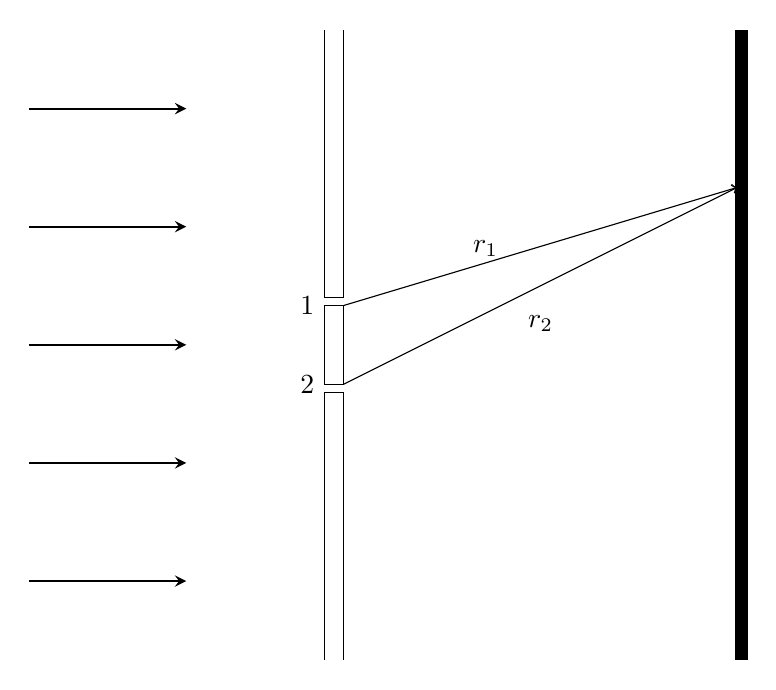
\begin{tikzpicture}
		\draw[ultra thick](5,-4)--(5,4);
		\draw[ultra thick](5.05,-4)--(5.05,4);
		\draw[ultra thick](5.1,-4)--(5.1,4);
		\draw(0,4)--(0,0.6)--(-0.25,0.6)--(-0.25,4);
		\draw(0,-4)--(0,-0.6)--(-0.25,-0.6)--(-0.25,-4);
		\draw(0,0.5)--(0,-0.5)--(-0.25,-0.5)--(-0.25,0.5)--(0,0.5);
		\draw[thick,-stealth](-4,3)--(-2,3);
		\draw[thick,-stealth](-4,1.5)--(-2,1.5);
		\draw[thick,-stealth](-4,-1.5)--(-2,-1.5);
		\draw[thick,-stealth](-4,-3)--(-2,-3);
		\draw[thick,-stealth](-4,0)--(-2,0);
		\node at(-0.25,0.5)[left]{$1$};
		\node at(-0.25,-0.5)[left]{$2$};
		\draw[->](0,0.5)--(5,2);
		\draw[->](0,-0.5)--(5,2);
		\node at(1.8,1)[above]{$r_1$};
		\node at(2.5,0.5)[below]{$r_2$};
	\end{tikzpicture}
	\caption{Doppia fenditura in assenza di campo magnetico.}
	\label{fig:fend1}
\end{figure} Se le particelle hanno impulso $\hbar k$, e se indichiamo con $\psi(1)$ e $\psi(2)$ i valori della funzione d'onda in prossimità delle due fenditure, allora in un punto dello schermo a distanza $r_1$ e $r_2$ rispettivamente dalla prima e dalla seconda fenditura si ha un'intensità
\[I\propto\left|\frac{\psi(1)}{r_1}e^{ikr_1}+\frac{\psi(2)}{r_2}e^{ikr_2}\right|^2\]
Abbiamo usato la solita approssimazione sulla distanza dallo schermo grande rispetto alle dimensioni della singola fenditura. Se poi anche la distanza tra queste è piccola rispetto alla distanza dallo schermo, possiamo ulteriormente approssimare e scrivere
\[I\propto\left|\psi(1)+\psi(2)e^{ik(r_2-r_1)}\right|^2\]
In assenza di campo, è ragionevole supporre $\psi(1)=\psi(2)$, quindi si ottiene semplicemente
\[I\propto\left|1+e^{ik(r_2-r_1)}\right|^2\]
Consideriamo ora la presenza di un campo magnetico: supponiamo che questo sia localizzato all'interno di un piccolo solenoide, posto all'interno dello schermo con le fenditure, come in figura \ref{fig:fend2}. In questa disposizione, classicamente non prevediamo alcun effetto, dato che il fascio non viene mai a contatto direttamente con il campo magnetico.
\begin{figure}[h!]
	\centering
	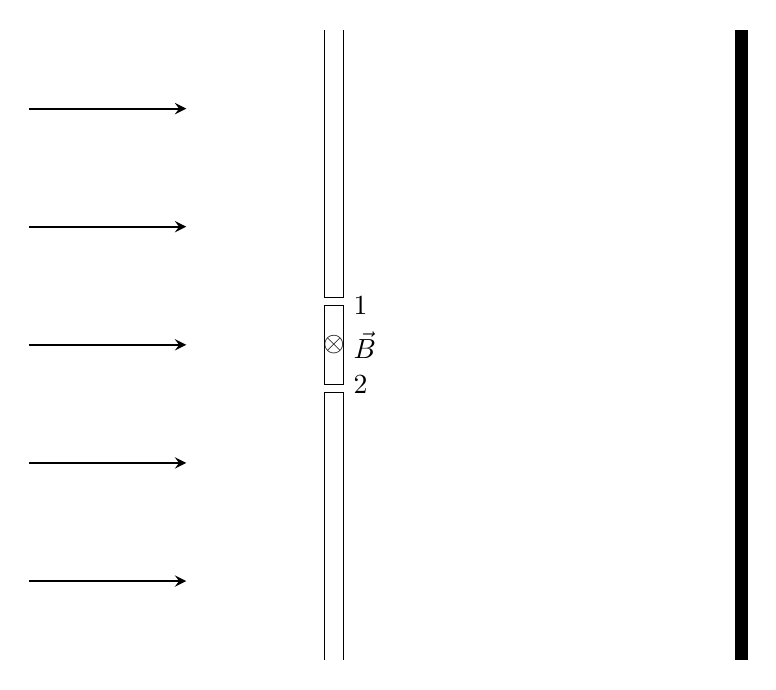
\begin{tikzpicture}
	\draw[ultra thick](5,-4)--(5,4);
	\draw[ultra thick](5.05,-4)--(5.05,4);
	\draw[ultra thick](5.1,-4)--(5.1,4);
	\draw(0,4)--(0,0.6)--(-0.25,0.6)--(-0.25,4);
	\draw(0,-4)--(0,-0.6)--(-0.25,-0.6)--(-0.25,-4);
	\draw(0,0.5)--(0,-0.5)--(-0.25,-0.5)--(-0.25,0.5)--(0,0.5);
	\draw[thick,-stealth](-4,3)--(-2,3);
	\draw[thick,-stealth](-4,1.5)--(-2,1.5);
	\draw[thick,-stealth](-4,-1.5)--(-2,-1.5);
	\draw[thick,-stealth](-4,-3)--(-2,-3);
	\draw[thick,-stealth](-4,0)--(-2,0);
	\node at(-0.125,0){$\otimes$};
	\node at(0,0)[right]{$\vec{B}$};
	\node at(0,0.5)[right]{$1$};
	\node at(0,-0.5)[right]{$2$};
	\end{tikzpicture}
	\caption{Doppia fenditura con campo magnetico.}
	\label{fig:fend2}
\end{figure}
Tuttavia, la presenza di $\vec{B}$ impedisce di avere $\vec{A}=0$ in tutto lo spazio: ci aspettiamo quindi un effetto sul pattern di interferenza. Effettivamente, possiamo supporre $\vec{A}=0$ a destra della fenditura e $\vec{A}\neq0$ a sinistra della fenditura. In tal modo, si ha ancora
\[I\propto\left|\psi(1)+\psi(2)e^{ik(r_2-r_1)}\right|^2\]
ma in generale non è più vero che $\psi(1)=\psi(2)$. Piuttosto, la differenza di fase tra le due funzioni d'onda è
\[\psi(2)=\exp\left(\frac{iq}{\hbar c}\int_{\Gamma(1)}\d \vec{s}\cdot\vec{A}(\vec{s})-\frac{iq}{\hbar c}\int_{\Gamma(2)}\d \vec{s}\cdot\vec{A}(\vec{s})\right)\psi(1)\]
dove $\Gamma(1)$ e $\Gamma(2)$ sono due percorsi qualunque che partono da un punto $\vec{x}_0$ a sinistra della fenditura e arrivano rispettivamente alla prima e alla seconda fenditura, rimanendo sempre contenuti nello spazio a sinistra del primo schermo. Dato che il potenziale vettore è nullo a destra, usando il teorema di Stokes si deduce
\[\psi(2)=\exp\left(\frac{iq}{\hbar c}\Phi(\vec{B})\right)\psi(1)\]
e dunque
\[I\propto\left|1+e^{ik(r_2-r_1)-iq\Phi(\vec{B})/\hbar c}\right|^2\]
Si ha quindi una traslazione rigida del pattern di interferenza, tranne nel caso in cui il flusso del campo magnetico sia quantizato come
\[\Phi(\vec{B})=n\frac{2\pi\hbar c}{q},\qquad n\in\Z\]
\subsubsection{Accoppiamento spin-campo magnetico e equazione di Pauli-Schr\"odinger}
In generale, se una particella ha anche un momento magnetico intrinseco $\bm{\mu}$, l'Hamiltoniana in presenza di campo magnetico è
\[\ham=\frac{1}{2m}\left(\op{\vec{p}}-\frac{q}{c}{\vec{A}}\right)^2+q\phi-\bm\mu\cdot\vec{B}\]
Il momento magnetico è proporzionale allo spin tramite
\[\bm{\mu}=\frac{\hbar qg}{2mc}\op{\vec{s}}\]
dove $g$ è un fattore adimensionale, noto come fattore giromagnetico. Vediamo una spiegazione ad hoc per tale Hamiltoniana, valida unicamente per particelle di spin $1/2$. In tal caso, lo spazio degli stati è isomorfo a
\[\H\cong\L^2(\R ^3)\otimes\C ^2\]
e dunque lo stato generico può essere messo nella forma
\[\psi=\left(\begin{array}{c}
\psi_+(\vec{x},t)\\\psi_-(\vec{x},t)
\end{array}\right)\]
Le due componenti di $\psi$ si interpretano poi come densità di probabilità per la particella di trovarsi in un certa posizione, in un certo istante, con una certa orientazione dello spin. Consideriamo ora un operatore vettoriale $\op{\vec{w}}$ su $\L^2(\R^3)$ e supponiamo che sia $[\op w_i,\op w_j]=0$. In realtà, tale operatore agisce sugli stati del sistema come l'operatore $\op{\vec{w}}\otimes\id_2$. Poniamo ora
\[\op{\vec{w}}\cdot\bm{\sigma}=\op w_i\otimes\sigma_i\]
In tal modo è
\[(\op{\vec{w}}\cdot\bm{\sigma})^2=\op{\vec{w}}^2\otimes\id_2\]
Questo significa che l'Hamiltoniana di particella libera
\[\ham=\frac{\op{\vec{p}}^2}{2m}\]
può anche essere scritta nella forma
\[\ham=\frac{(\op{\vec{p}}\cdot\bm{\sigma})^2}{2m}\]
Questa sostituzione non modifica nulla nella dinamica in assenza di campi. Viceversa, sotto accoppiamento minimale e in gauge di Lorenz si ha
\begin{align*}
	(\op{\vec{p}}\cdot\bm{\sigma})^2&\to\left[\left(\op{\vec{p}}-\frac{q}{c}\vec{A}\right)\cdot\bm{\sigma}\right]^2=\\&=\left[\left(\op{p}_i-\frac{q}{c}A_i\right)\left(\op{p}_j-\frac{q}{c}A_j\right)\right]\otimes(\sigma_i\sigma_j)=\\&=\left(\op{\vec{p}}-\frac{q}{c}\vec{A}\right)^2\otimes\id_2+i\varepsilon_{ijk}\left[\left(\op{p}_i-\frac{q}{c}A_i\right)\left(\op{p}_j-\frac{q}{c}A_j\right)\right]\otimes\sigma_k=\\&=\left(\op{\vec{p}}-\frac{q}{c}\vec{A}\right)^2\otimes\id_2-\frac{iq}{c}\left(\op{\vec{p}}\times\vec{A}+\vec{A}\times\op{\vec{p}}\right)\cdot\bm{\sigma}
\end{align*}
che porta infine a 
\[\ham=\frac{1}{2m}\left(\op{\vec{p}}-\frac{q}{c}\vec{A}\right)^2\otimes\id_2+q\phi-\frac{\hbar q}{2mc}\vec{B}\cdot\bm{\sigma}\]
Ricordando che per spin 1/2 è $\bm\sigma=2\op{\vec{s}}$, si trova anche $g=2$. Questo risultato è in accordo con la teoria di Dirac.
\subsection{Simmetrie discrete}
Abbiamo visto che a una simmetria continua di un sistema fisico $A$ corrisponde, tramite il teorema di Wigner, una famiglia continua di operatori unitari su $\H_A$, e tramite il teorema di Stone possiamo associare a questi operatori unitari dei generatori Hermitiani conservati durante l'evoluzione temporale. Per una simmetria discreta la trattazione è diversa e dipende fortemente dalla simmetria. Vedremo in dettaglio tre diverse simmetrie discrete.
\subsubsection{Parità}
Consideriamo l'applicazione lineare parità su $\R^3$, definita da
\[\mathcal{P}\vec{v}=-\vec{v}\]
Chiaramente $\mathcal{P}$ è idempotente, ossia $\mathcal{P}^2\vec{v}=\vec{v}$. A questa mappa facciamo corrispondere nello spazio di Hilbert del sistema l'operatore parità, che indichiamo con $\op{\mathcal{P}}$. Richiediamo che sugli autostati della posizione $\op{\mathcal{P}}$ agisca come
\[\op{\mathcal{P}}\ket{\vec{x}}=\ket{-\vec{x}}\]
Anche $\op{\mathcal{P}}$ è idempotente e lineare. Da questo si deduce l'azione della parità sulle funzioni d'onda, dato che
\[\op{\mathcal{P}}\ket{\psi}=\int\d^3\vec{x}\,\psi(\vec{x})\op{\mathcal{P}}\ket{\vec{x}}=\int\d^3\vec{x}\,\psi(\vec{x})\ket{-\vec{x}}\]
e dunque, posto $\op{\mathcal{P}}\ket{\psi}=\ket{\psi_{\mathcal{P}}}$ si ha
\[\psi_{\mathcal{P}}(\vec{x})=\psi(-\vec{x})\]
Allora $\op{\mathcal{P}}$ conserva i prodotti scalari, dato che
\[\braket{\varphi_{\mathcal{P}}}{\psi_{\mathcal{P}}}=\int \d^3\vec{x}\,\varphi^*(\vec{x})\psi(-\vec{x})=\braket{\varphi}{\psi}\]
e dunque per il teorema di Wigner l'operatore parità è unitario. L'azione della parità sugli operatori posizione e impulso è facilmente
\begin{align*}
	\op{\mathcal{P}}^\dagger\op{\vec{x}}\op{\mathcal{P}}&=-\op{\vec{x}}\\
	\op{\mathcal{P}}^\dagger\op{\vec{p}}\op{\mathcal{P}}&=-\op{\vec{p}}
\end{align*}
Infatti, per la posizione
\begin{align*}\op{\mathcal{P}}^\dagger\op{\vec{x}}\op{\mathcal{P}}\ket{\vec{x}}&=\op{\mathcal{P}}^\dagger\op{\vec{x}}\ket{-\vec{x}}=\\&=-\vec{x}\ket{\vec{x}}=\\&=-\op{\vec{x}}\ket{\vec{x}}\end{align*}
da cui per linearità si estende la proprietà a tutti gli stati $\ket{\psi}$. Per l'impulso l'azione sulle funzioni d'onda è
\begin{align*}
	\P^\dagger\op{\vec{p}}\P(\psi(\vec{x}))&=\P^\dagger\op{\vec{p}}(\psi(-\vec{x}))=\\&=-i\hbar\P^\dagger\nabla(\psi(-\vec{x}))=\\&=i\hbar\P^\dagger(\nabla\psi)(-\vec{x})=\\&=i\hbar\nabla\psi(\vec{x})=\\&=-\op{\vec{p}}\psi(\vec{x})
\end{align*}
Di conseguenza, la parità conserva le regole di commutazione canoniche, ossia
\[\P^\dagger[\op x_i,\op p_j]\P=[\op x_i,\op p_j]\]
Gli operatori vettoriali che sotto parità trasformano come $\op{\vec{x}}$ sono detti vettori veri, o, più brevemente, vettori. Altri operatori vettoriali possono trasformare in maniera diversa, ad esempio per il momento angolare è chiaramente
\[\P^\dagger\op{\vec{L}}\P=\op{\vec{L}}\]
Gli operatori vettoriali con questa legge di trasformazione sono noti come pseudovettori. Non abbiamo ancora definito l'azione di $\P$ sui gradi di libertà spinoriali del sistema: dato che il momento angolare totale è $\op{\vec{L}}+\op{\vec{s}}$, richiediamo che anche lo spin sia uno pseudovettore, ossia
\[\P^\dagger\op{\vec{s}}\P=\op{\vec{s}}\]
Di conseguenza, anche il momento magnetico $\op{\bm{\mu}}\propto\op{\vec{L}}+g\op{\vec{s}}$ è uno pseudovettore. Consideriamo ora un'Hamiltoniana $\ham$ invariante sotto parità, ossia
\[[\ham,\P]=0\]
Sappiamo allora che possiamo scegliere una base di autostati comuni di $\H$ e $\P$. Dato che la parità è idempotente, ha autovalori $\pm1$, e quindi gli stati a parità definita possono essere divisi in stati pari, ossia
\[\P\ket{\psi}=\ket{\psi}\]
e stati dispari, ossia
\[\P\ket{\psi}=-\ket{\psi}\]
Per vettori veri abbiamo quindi una regola di selezione molto forte: possono connettere solo autostati della parità con parità diversa.
\subsubsection{Traslazioni discrete}
Limitiamoci per semplicità a sistemi unidimensionali e consideriamo l'operatore di traslazione di $a$
\[\op T=e^{-i\op{p}a/\hbar}\]
La sua azione sulla posizione e sull'impulso sono
\begin{align*}\op T^\dagger\op x\op T&=\op x+a\\\op T^\dagger\op p\op T=\op p\end{align*}
Supponiamo ora di avere un'Hamiltoniana $\ham$ invariante sotto questa traslazione. Se
\[\ham=\frac{\op p^2}{2m}+V(\op x)\]
questo significa che il potenziale è periodico di periodo $a$. Vale allora il teorema di Bloch, ossia le autofunzioni di $\ham$ possono essere scelte della forma
\[\psi(x)=e^{ikx}u_k(x)\]
dove $k\in[-\pi/a,\pi/a]$ e dove $u_k$ è una funzione periodica di periodo $a$. Per la dimostrazione, sappiamo che
\[\ham,\op T]=0\]
quindi possiamo diagonalizzare simultaneamnte l'Hamiltoniana e l'operatore di traslazione. Per quest'ultimo $\op T^\dagger=\op T^{-1}$, dunque gli autovalori di $\op{T}$ hanno norma 1. Se
\[\op T\ket{\psi}=e^{i\theta}\ket{\psi}\]
per $\theta\in[-\pi,\pi]$, allora per le funzioni d'onda
\[\psi(x-a)=e^{i\theta}\psi(x)\]
Supponiamo ora che $\ket{\psi}$ sia anche un autostato dell'Hamiltoniana, e poniamo
\[k=-\frac{\theta}{a},\qquad\qquad u_k(x)=e{-ikx}\psi(x)\]
In tal modo è
\[u_k(x-a)=e^{-ik(x-a)}\psi(x-a)=u_k(x)\]
come voluto.

L'equazione di Schr\"odinger indipendente dal tempo è allora
\[u_k''(x)+2iku_k'(x)=\left[\frac{2m}{\hbar^2}\left(V(x)-E\right)+k^2\right]u_k(x)\]
In generale, a $k$ fissato avremo uno spettro $E=E_n(k)$. Se ora fissiamo $n$, è ragionevole che $E_n(k)$ sia una funzione (almeno) continua di $k$, cioè i livelli energetici del sistema sono organizzati in bande.
\subsubsection{Inversione temporale}
Consideriamo una Hamiltoniana $\ham$ indipendente dal tempo e sia $\ket{\psi(t)}$ una soluzione dell'equazione di Schr\"odinger
\[i\hbar\pder{}{t}\ket{\psi(t)}=\ham\ket{\psi(t)}\]
Sia $\ket{\psi\ped{rev}(t)}$ lo stato con funzione d'onda
\[\psi\ped{rev}(\vec{x},t)=\psi^*(\vec{x},-t)\]
Tale stato è ancora soluzione dell'equazione di Schr\"odinger. La densità di probabilità per le misure di posizione è facilmente
\[P\ped{rev}(\vec{x},t)=P(\vec{x},-t)\]
Per le misure di impulso dobbiamo invece fare la trasformata di Fourier di $\psi\ped{rev}$, dunque si ottiene
\[P\ped{rev}(\vec{p},t)=P\ped{rev}(-\vec{p},-t)\]
Consideriamo ora la mappa $\ket{\psi(t)}\mapsto\ket{\psi\ped{rev}(-t)}$, che ha le proprietà che vogliamo classicamente da un'inversione temporale. Tale mappa conserva i moduli dei prodotti scalari, esplicitamente, è
\[\braket{\varphi\ped{rev}(t)}{\psi\ped{rev}(t)}=\braket{\psi(t)}{\varphi(t)}\]
e dunque la mappa in questione è antiunitaria. Consideriamo ora un operatore $\T$ definito sugli autostati della posizione da
\[\T\ket{\vec{x}}=\ket{\vec{x}}\]
Se richiediamo che $\T$ sia antilineare, allora su un generico stato $\ket{\psi(t)}$ agisce come
\[\T\ket{\psi(t)}=\T\int \d^3\vec{x}\,\psi(\vec{x},t)\ket{\vec{x}}=\int\d^3\vec{x}\,\psi^*(\vec{x},t)\ket{\vec{x}}\]
ossia
\[\T\ket{\psi(t)}=\ket{\psi\ped{rev}(-t)}\]
Tale operatore è idempotente e trasforma la posizione e l'impulso come
\[\T^\dagger\op{\vec{x}}\T=\op{\vec{x}},\qquad\qquad\T^\dagger\op{\vec{p}}\T=-\op{\vec{p}}\]
In particolare, non conserva le relazioni di commutazione canoniche
\[\T^\dagger[\op x_i,\op p_j]\T=-[\op x_i,\op p_j]\]
Inoltre, il momento angolare trasforma come
\[\T^\dagger\op{\vec{L}}\T=-\op{\vec{L}}\]
Supponiamo ora di avere un'Hamiltoniana $\H$ che commuti con $\T$. Allora se $\ket{\psi}$ è un autostato dell'Hamiltoniana a energia $E$, anche $\T\ket{\psi}$ lo è. Se il livello è non degenere deve essere
\[\T\ket{\psi}=\lambda\ket{\psi}\]
per qualche $\lambda\in\C$. Dato che $\T$ è idempotente, deve essere $|\lambda|=1$, ossia $\lambda=e^{i\theta}$. Allora per la funzione d'onda è
\[\psi^*(x)=e^{i\theta}\psi(x)\]
ossia la fase della funzione d'onda è uniforme in $x$. Questo implica chiaramente che la funzione d'onda può essere scelta reale.

Vediamo ora l'azione di $\T$ sullo spin. Vogliamo che il momento angolare totale sia ancora il generatore delle rotazioni, quindi richiediamo
\[\T^\dagger\op{\vec{s}}\T=-\op{\vec{s}}\]
Gli stati del sistema sono ora della forma $\ket{\vec{x};s,m}$. Su questi stati si ha
\[\T\ket{\vec{x};s,m}=(-)^{s-m}\ket{\vec{x};s,-m}\]
Per mostrare questa proprietà, supponiamo che sia
\[\T\ket{\psi}=e^{-i\pi \op{s}_2/\hbar}\op K_0\ket{\psi}\]
dove $\op{K}_0$ è un operatore antilineare che commuta con $\op s_2$ e tale che
\[\op{K}_0\ket{\vec{x};s,m}=\ket{\vec{x};s,m}\]
Chiaramente $\op{K}_0$ è idempotente. Se la decomposizione di $\T$ è possibile, allora su uno stato $\ket{\psi}=\alpha_{\vec{x},s,m}\ket{\vec{x};s,m}$ è
\begin{align*}
	\T^{-1}\op s_j\T\ket{\psi}&=\sum_{\vec{x},s,m}\alpha_{\vec{x};s,m}\T^{-1}\op s_j\T\ket{\vec{x};s,m}=\\&=\sum_{\vec{x},s,m}\op K_0e^{i\pi\op s_2/\hbar}\op s_je^{-i\pi\op s_2/\hbar}\op K_0\ket{\vec{x};s,m}=\\&=(-)^j\op K_0\op s_j\op K_0\ket{\psi}
\end{align*}
Infatti, se $j=2$ la soluzione è banale. Se $j\neq2$ allora stiamo ruotando $\op s_j$ di $\pi$ intorno all'asse $2$, quindi compare un segno $-$. A questo punto è sufficiente mostrare 
\[e^{-i\pi \op s_2/\hbar}\ket{\vec{x};s,m}=(-)^{s-m}\ket{\vec{x};s,-m}\]
Chiaramente è
\[e^{-i\pi\op s_2/\hbar}\ket{\vec{x};s,m}=e^{i\theta(s,m)}\ket{\vec{x};s,-m}\]
dato che per un rotazione di $\pi$ intorno all'asse 2 la componente $\op s_3$ cambia segno. Ora, per $s=1/2$ si verifica a mano che la fase è proprio $(-)^{s-m}$. Per $s$ generico basta ricordare che la rappresentazione di spin $s$ è contenuta all'interno della rappresentazione $(1/2)^{\otimes N}$ per $N$ sufficientemente grande.

Inoltre, se la decomposizione di $\T$ è possibile allora è
\[\T^2=e^{-2\pi i\op s_2/\hbar}=(-)^{2s}\id\]
cioè il time reversal è idempotente solo per particelle con spin intero. Questo fatto implica un'importante risultato, noto come teorema di Kramers: un'Hamiltoniana $\ham$ di un sistema con spin semintero invariante sotto $\T$ ammette autovalori almeno doppiamente degeneri. Infatti, supponiamo per assurdo che $\ket{\psi}$ sia un autostato a energia $E$ di $\ham$ non degenere. Allora è
\[\ham\T\ket{\psi}=E\T\ket{\psi}\]
dato che $E$ è reale. Allora deve essere $\T\ket{\psi}=\lambda\ket{\psi}$, ma questo implica
\[-\ket{\psi}=\T^2\ket{\psi}=|\lambda|^2\ket{\psi}\]
e questo è assurdo.%FINISCI
\subsection{Sistemi a molte particelle}
Consideriamo un sistema \emph{classico} di $N$ particelle uguali, ossia caratterizzate dalle stesse proprietà fisiche, come massa e carica elettrica. L'Hamiltoniana del sistema deve essere simmetrica sotto lo scambio di due particelle qualunque, ma a rigore queste particelle sono sempre distinguibili, nel senso che sotto l'evoluzione temporale è possibile seguire l'evoluzione della singola particella. In altre parole, le condizioni iniziali del sistema ci forniscono delle etichette per distinguere le particelle. Questa distinguibilità è intrinsecamente legata al fatto che in una teoria classica è possibile parlare di traiettorie.

In meccanica quantistica non è possibile fare lo stesso: particelle con le stesse proprietà fisiche sono a tutti gli effetti indistinguibili. I sistemi con più di una particella richiedono quindi una trattazione particolare e, come vedremo, l'introduzione di un ulteriore assioma nella teoria. Per capirne il motivo, consideriamo lo spazio di Hilbert $\H$ degli stati di una singola particella. Immaginiamo ora di avere due regioni spaziali $1$ e $2$ molto lontane spazialmente. In tal modo, se $\ket{u}\in\H$ è lo stato associato a un pacchetto ben localizzato nella zona $1$ e $\ket{v}\in\H$ è lo stato associato a un pacchetto ben localizzato nella zona $2$, possiamo supporre
\[\braket{u}{v}=0\]
Consideriamo ora due particelle identiche e supponiamo che a $t=0$ una particella (identificata con la lettera $A$) sia nella zona 1, l'altra particella (identificata con la lettera $B$) sia nella zona 2. Gli spazi di Hilbert di singola particella sono chiaramente $\H_A\cong\H_B\cong\H$, mentre gli stati del sistema appartengono a $\H_A\otimes\H_B$. Dato che le particelle sono in realtà indistinguibili, le etichette $A$ e $B$ non possono davvero essere introdotte. In altre parole, lo stato iniziale del sistema è indifferentemente $\ket{u}_A\otimes\ket{v}_B$ o $\ket{v}_A\otimes\ket{u}_B$, o una combinazione lineare di questi, ossia
\[\ket{\psi}_{AB}=\alpha\ket{u}_A\otimes\ket{v}_B+\beta\ket{v}_A\otimes\ket{u}_B\]
Se ora $\ket{u}'\in\H$ è uno stato ben localizzato nella zona 1\footnote{Quindi ortogonale a $\ket{v}$.}, la probabilità che una particella sia nello stato $\ket{u'}$ è il valor medio dell'operatore
\[\op{T}=\ket{u'}_A\bra{u'}\otimes\id_B+\id_A\otimes\ket{u'}_B\bra{u'}\]
e dunque si ha facilmente
\[P(1,\ket{u'})=|\braket{u'}{u}|^2\]
Questo risultato è aspettato, ma non permette di distinguere tra i diversi valori di $\alpha$ e $\beta$. Supponiamo ora di accendere un'Hamiltoniana $\ham$ identica per le due particelle, e che queste siano non interagenti. L'Hamiltoniana totale è allora
\[\ham_{AB}=\ham\otimes\id_B+\id_A\otimes\ham\]
Lo stato iniziale evolve allora come ($\hbar=1$)
\[\ket{\psi(t)}_{AB}=e^{-i\ham_{AB}t}\ket{\psi}_{AB}=\alpha\left(e^{-i\ham t}\ket{u}_A\right)\otimes\left(e^{-i\ham t}\ket{v}_B\right)+\beta\left(e^{-i\ham t}\ket{v}_A\right)\otimes\left(e^{-i\ham t}\ket{u}_B\right)\]
Possiamo scegliere $\ham$ in modo tale che gli stati iniziali inizino a "diffondere" nella regione tra la zona 1 e la zona 2. In altre parole, se $\ket{0}\in\H$ è uno stato con overlap non nullo sia con $\ket{u}$ che con $\ket{v}$, possiamo chiedere quale sia la probabilità di trovare entrambe le particelle dopo un tempo $t$ nello stato $\ket{0}$. L'unico stato del sistema congiunto con entrambe le particelle in questo stato è manifestamente $\ket{0}_A\otimes\ket{0}_B$, dunque si trova
\[P(2,\ket{0},t)=|\alpha+\beta|^2\left|\braketop{0}{e^{-i\ham t}}{u}
\right|^2\left|\braketop{0}{e^{-i\ham t}}{v}
\right|^2\]
Adesso l'esito della misura \emph{dipende} dai valori di $\alpha$ e $\beta$. Dobbiamo quindi trovare un modo per fissare i loro valori, in caso contrario la nostra teoria non sarebbe predittiva. Per fare ciò, diamo qualche definizione e risultato preliminari. Innanzitutto, per $N$ particelle dobbiamo considerare lo spazio di Hilbert $\H_N=\H^{\otimes N}$. In tal caso, se $\sigma\in S_N$ è una permutazione delle particelle, definiamo su $\H_N$ l'operatore $\op P_\sigma$ definito sui vettori decomponibili da
\[\op P_\sigma\ket{\phi_1}_1\otimes\ldots\otimes\ket{\phi_N}_N=\ket{\phi_{\sigma(1)}}_1\otimes\ldots\otimes\ket{\phi_{\sigma(N)}}_N\]
In particolare, se $\sigma=(\begin{array}{c c}
1&2
\end{array})$ e se $\left\{\ket{j}\right\}$ è una base di $\H$ si ha
\[\op P_\sigma=\sum_{j,j'}\ket{j}_1\bra{j'}\otimes\ket{j'}_2\bra{j}\otimes\id_3\otimes\ldots\otimes\id_N\]
e similmente per le altre trasposizioni. Si noti ora che una trasposizione è idempotente, dunque ha autovalori $\pm1$. Diciamo che un vettore $\ket{\psi}\in\H_N$ è completamente simmetrico se per ogni trasposizione $\tau\in S_N$ si ha
\[\op{P}_\tau\ket{\psi}=\ket{\psi}\]
e similmente diciamo che $\ket{\psi}$ è completamente simmetrico se per ogni trasposizione $\tau\in S_N$ si ha
\[\op{P}_\tau\ket{\psi}=-\ket{\psi}\]
Le definizioni sono equivalenti a
\[\op{P}_\sigma\ket{\psi}=\ket{\psi},\qquad\qquad\op{P}_\sigma\ket{\psi}=(\mathrm{sgn}\,\sigma)\ket{\psi}\]
dove $\sigma$ è una permutazione qualunque. \`{E} noto che i vettori completamente simmetrici formano un sottospazio di $\H_N$, detto potenza simmetrica e indicato con $\H_N^{(\textrm{sym})}$, di dimensione
\[\dim\H_N^{(\textrm{sym})}=\binom{d+N-1}{N}\]
dove $d=\dim\H$. Il proiettore $\op{\Pi}^{(\textrm{sym})}\colon\H_N\to\H_N^{(\textrm{sym})}$ è
\[\op{\Pi}^{(\textrm{sym})}=\frac{1}{N!}\sum_{\sigma\in S_N}\op P_\sigma\]
Similmente, i vettori completamente antisimmetrici formano un sottospazio di $\H_N$ noto come potenza esterna, e indicato con $\H_N^{(\textrm{anti})}$. La dimensione di tale sottospazio è non nulla solo per $N\leq d$, in particolare
\[\dim\H_N^{(\textrm{anti})}=\binom{d}{N}\]
Il proiettore $\op{\Pi}^{(\textrm{anti})}\colon\H_N\to\H_N^{(\textrm{anti})}$ è
\[\op{\Pi}^{(\textrm{anti})}=\frac{1}{N!}\sum_{\sigma\in S_N}(\mathrm{sgn}\,\sigma)\op P_\sigma\]
Si noti che la decomposizione $\H_N=\H_N^{(\textrm{sym})}\oplus\H_N^{(\textrm{anti})}$ vale solo per $N=2$. Infatti, per $N>2$ possiamo avere dei vettori decomponibili con simmetria mista, ossia pari sotto lo scambio di alcune componenti e dispari sotto lo scambio di altre componenti\footnote{Come è chiaro dalle tabelle di Young di $S_N$.}. Siamo ora pronti a dare l'assioma di simmetrizzazione.
\paragraph{Assioma di simmetrizzazione} Se $\H$ è lo spazio di Hilbert di singola particella, gli stati di un sistema di $N$ particelle sono associati ai vettori di $\H^{\otimes N}$ che sono completamente simmetrici o completamente antisimmetrici. Nel primo caso si parla di bosoni, nel secondo di fermioni. Inoltre, le osservabili sono tutti e soli gli operatori $\op\Theta$ autoaggiunti tali che per ogni $\sigma\in S_N$ si abbia
\[\op P_\sigma^\dagger\op{\Theta}\op P_\sigma=\op{\Theta}\]

In particolare, supponiamo di avere un sistema bosonico di $N$ particelle in cui sappiamo che una particella è nello stato $\ket{\phi_1}$, un'altra particella dello stato $\ket{\phi_2}$, e così via. Allora lo stato del sistema è
\[\ket{\psi}_N=\op{\Pi}^{(\mathrm{sym})}\ket{\phi_1}_1\otimes\ldots\otimes\ket{\phi_N}_N\]
e similmente nel caso fermionico. Per i fermioni vale inoltre chiaramente il principio di esclusione di Pauli: se proviamo ad avere due fermioni nello stesso stato, allora lo stato del sistema è nullo. In altre parole, non possiamo avere tutti i numeri quantici uguali per due fermioni indistinguibili. 

Vediamo ora qualche conseguenza sugli stati finali di uno scattering di due particelle. Supponiamo di avere a $t=0$ una particella nello stato $\ket{u}$ e una particella nello stato $\ket{v}$. Lo stato iniziale è dunque
\[\ket{\psi}=\frac{\ket{u}_A\otimes\ket{v}_B\pm\ket{v}_A\otimes\ket{u}_B}{\sqrt{2}}\]
dove il segno $+$ è per i bosoni. Supponiamo, come prima, che $\ket{u}$ sia concentrato nella zona 1 e $\ket{v}$ sia concentrato nella zona 2. Similmente, immaginiamo di avere due detector, uno per zona. Sia $\ket{a}$ lo stato che viene rilevato dal detector nella zona 1. Siamo ragionevolmente sicuri che questo stato corrisponda a un pacchetto che non si sovrappone alla zona 2. Allo stesso modo, sia $\ket{b}$ lo stato rilevato dal detector nella zona 2. Allora lo stato rilevato dai due detector congiunti è
\[\ket{\psi\ped{target}}=\frac{\ket{a}_A\otimes\ket{b}_B\pm\ket{b}_A\otimes\ket{a}_B}{\sqrt{2}}\]
dove, di nuovo, il segno $+$ è per i bosoni. La probabilità che il detector scatti al tempo $t$ è allora
\[P(t)=|\braket{\psi\ped{target}}{\psi(t)}|^2=|\braket{a}{u(t)}\braket{b}{v(t)}\pm\braket{a}{v(t)}\braket{b}{u(t)}|^2\]
Siamo cioè in grado di distinguere i due tipi di particelle. Se invece avessimo delle particelle distinguibili, non dobbiamo simmetrizzare le funzioni d'onda e allora si ottiene semplicemente
\[P(t)=|\braket{a}{u(t)}\braket{b}{v(t)}|^2+|\braket{a}{v(t)}\braket{b}{u(t)}|^2\]
che è ancora diversa dalle statistiche precedenti. Se ora riprendiamo l'esempio precedente sullo stato $\ket{0}$ "diffuso" nella regione tra la zona 1 e la zona 2, la probabilità che entrambe le particelle siano entrambe in $\ket{0}$ è
\[P(t)=\begin{cases}0&\textrm{ per fermioni}\\
2|\braket{0}{u(t)}\braket{0}{v(t)}|^2&\textrm{ per bosoni}\\
|\braket{0}{u(t)}\braket{0}{v(t)}|^2&\textrm{ per particelle distinguibili}
\end{cases}\]
Visti i risultati, si parla di antibunching di fermioni e di bunching di bosoni.

Concludiamo con un'osservazione cruciale: a rigore, il principio di simmetrizzazione vale per tutte le particelle identiche dello stesso tipo. Questo significa che gli operatori di simmetrizzazione vanno applicati allo spazio $\H_N$, dove $N$ è il numero di particelle dell'intero universo. Ad esempio, se consideriamo un atomo con più elettroni, la funzione d'onda elettronica si ottiene antisimmetrizando la funzione d'onda di tutti gli elettroni dell'universo, non solo di quelli atomici. Sembra quindi che ogni caso concreto sia di fatto intrattabile, sia per il numero enorme di particelle dello stesso tipo in giro per l'universo, sia per la nostra ignoranza sul loro stato. Vediamo come risolvere questo dilemma. Consideriamo un sistema di $N$ particelle identiche, e consideriamo un suo sottosistema di $n$ particelle. Supponiamo, per fissare le idee, di lavorare con fermioni: il caso bosonico è del tutto analogo. Lo stato del sottosistema è allora un vettore completamente antisimmetrico $\ket{\chi}_{1,\ldots,n}\in\H_n^{(\textrm{anti})}$, mentre lo stato delle particelle al di fuori del sottosistema è un vettore completamente antisimmetrico $\ket{\psi}_{n+1,\ldots,N}\in\H_{N-n}^{(\textrm{anti})}$. Al solito, supponiamo che stati appartenenti a sottosistemi diversi siano ortogonali. Lo stato del sistema è allora
\[\ket{\phi}_{1,\ldots,N}=\lambda\op{\Pi}^{(\textrm{anti})}\ket{\chi}_{1,\ldots,n}\otimes\ket{\psi}_{n+1,\ldots,N}\]
dove $\op{\Pi}^{(\textrm{anti})}$ è l'operatore di antisimmetrizzazione su $\H_N$ e dove $\lambda$ è una costante di normalizzazione. Vediamo come calcolare $\lambda$. Si ricordi che
\[\op{\Pi}^{(\textrm{anti})}\ket{\chi}_{1,\ldots,n}\otimes\ket{\psi}_{n+1,\ldots,N}=\frac{1}{N!}\sum_{\sigma\in S_N}(\mathrm{sgn}\,\sigma)\op P_{\sigma}\ket{\chi}_{1,\ldots,n}\otimes\ket{\psi}_{n+1,\ldots,N}\]
Tra queste permutazioni possiamo individuare alcune permutazioni più belle, ossia quelle che non mischiano i primi $n$ indici con i successivi. Più in generale, si ricordi la decomposizione in cicli di una permutazione $\sigma$. Possiamo riordinare i cicli mettendo $\sigma$ nella forma
\[\sigma=\sigma\ped{mixed}\sigma_n\sigma_{N-n}\]
dove $\sigma_n$ è un prodotto di cicli di interi contenuti in $\left\{1,\ldots,n\right\}$, $\sigma_{N-n}$ è un prodotto di cicli di interi contenuti in $\left\{n+1,\ldots,N\right\}$, e infine $\sigma\ped{mixed}$ è il prodotto dei cicli che mescolano indici tra i due insiemi. Chiaramente $\sigma\ped{mixed}$, $\sigma_n$ e $\sigma_{N-n}$ commutano tra loro e inoltre si ha
\[\op P_\sigma\ket{\chi}_{1,\ldots,n}\otimes\ket{\psi}_{n+1,\ldots,N}=(\mathrm{sgn}\,\sigma_n\mathrm{sgn}\,\sigma_{N-n})\op P_{\sigma\ped{mixed}}\ket{\chi}_{1,\ldots,n}\otimes\ket{\psi}_{n+1,\ldots,N}\]
Perchè gli operatori $\op P_\tau$ sono una rappresentazione di $S_n$ e perchè gli stati su $\H_n$ e $\H_{N-n}$ sono già antisimmetrizzati. Allora è semplicemente
\begin{align*}\op{\Pi}^{(\textrm{anti})}\ket{\chi}_{1,\ldots,n}\otimes\ket{\psi}_{n+1,\ldots,N}&=\frac{1}{N!}\sum_{\sigma\in S_N}(\mathrm{sgn}\,\sigma\ped{mixed})\op P_{\sigma\ped{mixed}}\ket{\chi}_{1,\ldots,n}\otimes\ket{\psi}_{n+1,\ldots,N}=\\&=\frac{n!(N-n)!}{N!}\sum_{\sigma\ped{mixed}\in S_N}(\mathrm{sgn}\,\sigma\ped{mixed})\op P_{\sigma\ped{mixed}}\ket{\chi}_{1,\ldots,n}\otimes\ket{\psi}_{n+1,\ldots,N}\end{align*}
Quindi la norma cercata è, ricordando l'hermitianità e l'idempotenza dei proiettori
\[\bra{\chi}_{1,\ldots,n}\otimes\bra{\psi}_{n+1,\ldots,N}\op{\Pi}^{(\textrm{anti})}\ket{\chi}_{1,\ldots,n}\otimes\ket{\psi}_{n+1,\ldots,N}=\frac{n!(N-n)!}{N!}\]
Perchè ogni permutazione $\sigma\ped{mixed}$ diversa dall'identità genera uno stato ortogonale a $\ket{\chi}_{1,\ldots,n}\otimes\ket{\psi}_{n+1,\ldots,N}$. Questo significa che gli stati del sistema sono della forma
\[\ket{\phi}_{1,\ldots,N}={\binom{N}{n}}^{1/2}\op{\Pi}^{(\textrm{anti})}\ket{\chi}_{1,\ldots,n}\otimes\ket{\psi}_{n+1,\ldots,N}\]
Consideriamo ora un'osservabile locale su $\H_n$. Possiamo supporre senza perdita di generalità che sia un proiettore $\ket{\zeta}_{1,\ldots,n}\bra{\zeta}_{1,\ldots,n}$. Fissata una base $\left\{\ket{\psi_i}_{n+1,\ldots,N}\right\}_i$ di $\H_{N-n}$, allora il valor medio della nostra osservabile è chiaramente
\[\sum_i\binom{N}{n}\left|\bra{\zeta}_{1,\ldots,n}\otimes\bra{\psi_i}_{n+1,\ldots,N}\op{\Pi}^{\textrm{(anti)}}\op{\Pi}^{\textrm{(anti)}}\ket{\chi}_{1,\ldots,n}\otimes\ket{\psi}_{n+1,\ldots,N}\right|^2\]
di nuovo, le uniche permutazioni rilevanti sono le $\sigma\ped{mixed}$, e di nuovo tra queste solo l'identità dà un contributo non nullo, pari a 
\[\sum_{i}|\braket{\zeta}{\chi}|^2|\braket{\psi_i}{\psi}|^2=\braket{\zeta}{\chi}|^2\]
Ma questo significa che le medie sul solo sottosistema sono le stesse che si ottengono facendo mediando sull'intero sistema, che è proprio quello che vogliamo dalla teoria.

Vediamo infine, come esempio, il caso di due particelle di spin $1/2$. Lo spazio di Hilbert di singola particella è $\H=\H\ped{orb}\otimes\H\ped{spin}$, dove $\H\ped{spin}\cong\C^2$. Lo spazio di Hilbert di due particelle è, al solito, $\H^{\otimes 2}$ e dobbiamo selezionare all'interno di questo spazio i soli stati antisimmetrici. Ci si convince facilmente che gli stati del sistema a due particelle sono allora della forma
\[\ket{\psi}=\ket{\phi\ped{anti}}\otimes\ket{\chi\ped{sym}}+\ket{\phi\ped{sym}}\otimes\ket{\chi\ped{anti}}\]
dove $\ket{\phi\ped{anti}}\in\op{\Pi}^{(\textrm{anti})}\H^{\otimes2}\ped{orb}$, $\ket{\phi\ped{sym}}\in\op{\Pi}^{(\textrm{sym})}\H^{\otimes2}\ped{orb}$, $\ket{\chi\ped{anti}}\in\op{\Pi}^{(\textrm{anti})}\H^{\otimes2}\ped{spin}$ e $\ket{\chi\ped{sym}}\in\op{\Pi}^{(\textrm{sym})}\H^{\otimes2}\ped{spin}$. In particolare, deve essere
\[\ket{\chi\ped{anti}}=\frac{\ket{\uparrow\downarrow}-\ket{\downarrow\uparrow}}{\sqrt{2}}\]
mentre $\ket{\chi\ped{sym}}$ è uno stato del tripletto.
\subsection{Cenni alla seconda quantizzazione}
In questa sezione diamo una breve introduzione alla seconda quantizzazione, che permette di trattare i sistemi a molte particelle in maniera equivalente a quanto fatto nella sezione precedente, ma ha diversi vantaggi e sviluppi che saranno visti in altri corsi. Partiamo dal caso bosonico. Si ricordi che nel precedente approccio, ossia nella prima quantizzazione, se abbiamo $N$ bosoni tali che ci siano $n_1$ bosoni nello stato $\ket{u_1}$ di singola particella, e così via fino a $n_k$ bosoni nello stato $\ket{u_k}$ di singola particella, allora lo stato del sistema è 
\[\ket{\psi}\propto\op{\Pi}^{(\textrm{sym})}\ket{u_1}^{\otimes n_1}\ldots\ket{u_k}^{\otimes n_k}\]
con, chiaramente, il vincolo $n_1+\ldots+n_k=N$.

Nella seconda quantizzazione si "evita" di passare dagli stati di singola particella per definire lo stato del sistema. Più precisamente, gli stati del sistema appartengono a uno spazio di Hilbert $\H\ped{Fock}$, detto spazio di Fock, i cui stati sono della forma
\[\ket{n_1,u_1;n_2,u_2;\ldots;n_k,u_k}\]
dove $n_1,\ldots,n_k$ sono i cosiddetti numeri di occupazione, che indicano quante particelle siano presenti in un dato stato di singola particella. Supponiamo ora che gli stati di singola particella considerati formino un base dello spazio di Hilbert di singola particella.

La differenza dal precedente approccio è notevole: nella prima quantizzazione di fatto si suppone temporaneamente che le particelle siano distinguibili, e poi si cercano dei metodi per evitare di contare gli stati del sistema più volte. D'altra parte, in seconda quantizzazione abbiamo già a che fare con stati simmetrici, dato che siamo interessati unicamente ai numeri di occupazione e non ci concentriamo mai sulle singole particelle. Non dobbiamo dunque neanche introdurre i fastidiosi operatori di simmetrizzazione e le costanti di normalizzazione. 

L'idea alla base della seconda quantizzazione (per sistemi bosonici) è l'identificazione di uno stato di vuoto $\ket0$ all'interno dello spazio di Fock. Da questo possiamo costruire gli stati con numeri di occupazione diversi introducendo degli operatori $\op{a}_j$ analoghi agli operatori di distruzione dell'oscillatore armonico. In particolare, le regole di commutazione di questi operatori sono
\[[\op a_i,\op a_j]=0,\qquad\qquad[\op a_i,\op a_j^\dagger]=\delta_{ij}\]
e usando questi operatori gli stati del sistema con una sola particella sono
\[\ket{1,u_j}=\op a_j^\dagger\ket{0}\]
In particolare, se in prima quantizzazione abbiamo uno stato di una particella
\[\ket{\psi}=\sum_j\alpha_j\ket{u_j}\]
allora in seconda quantizzazione abbiamo lo stato
\[\sum_j\alpha_j\ket{1,u_j}=\left(\sum_j\alpha_j\op{a}_j^\dagger\right)\ket0\]
Questa costruzione sembra dipendere da quale base dello spazio di Hilbert di singola particella abbiamo scelto. Se fissiamo un'altra base $\left\{\ket{v_j}\right\}$, possiamo definire gli operatori $\op b_j$ analoghi agli $\op a_j$ nella base precedente, ossia
\[\ket{1,v_j}=\op b_j^\dagger\ket0\]
e con le solite regole di commutazione
\[[\op b_i,\op b_j]=0,\qquad\qquad[\op b_i,\op b_j^\dagger]=\delta_{ij}\]
Chiaramente si ha
\[\ket{v_j}=\sum_k\ket{u_k}\braket{u_k}{v_j}\]
Richiediamo che anche gli operatori cambino allo stesso modo, ossia
\[\op b_j^\dagger=\sum_k\op a_k^\dagger\braket{u_k}{v_j}\]
In tal modo le ampiezze sono indipendenti dalla base scelta, e inoltre anche le regole di commutazione sono consistenti.

Per più particelle, si ha chiaramente
\[\ket{n_1,u_1;\ldots;n_k,u_k}=(\op a_1^{\dagger})^{n_1}\ldots(\op a_k^\dagger)^{n_k}\ket0\]
e l'ordine in cui compaiono gli operatori $\op a^\dagger_j$ non conta, ossia lo stato è già simmetrico, come volevamo. Si nota facilmente che gli operatori $\op a_i$ consentono di distruggere una particella, in analogia con quanto accade nell'oscillatore armonico.

Per il caso fermionico la trattazione è simile: si introducono gli operatori $\op a_j$, ma con le regole di commutazione
\[\{\op a_i,\op a_j\}=0,\qquad\qquad\{\op a_i,\op a_j^\dagger\}=1\]
In tal modo, posto
\[\ket{n_1,u_1;\ldots;n_k,u_k}=(\op a_1^{\dagger})^{n_1}\ldots(\op a_k^\dagger)^{n_k}\ket0\]
l'antisimmetria della funzione d'onda è assicurata, dato che $\op a_j^2=0$.

Per un sistema misto di bosoni e fermioni si fa lo stesso, ossia si introducono gli operatori di creazione $\op a_j^\dagger$ per i bosoni, gli operatori di creazione $\op b_j^\dagger$ per i fermioni, e si richiede oltre alle usuali regole di commutazione
\[[\op a_i,\op b_j]=0\]

Veniamo ora alle osservabili. Avevamo visto che in prima quantizzazione tutte le osservabili sono simmetriche sotto lo scambio di particelle, dunque se $\op R_j$ è l'operatore associato all'osservabile $R$ sulla $j$-esima particella, sull'intero sistema si deve considerare l'operatore
\[\op R^{(N)}=\sum_{j=1}^{N}\op R_j\]
Se decomponiamo $\op R$ nella base precedente, ossia se
\[\op R=\sum_{i,j}r_{ij}\ket{u_i}\bra{u_j}\]
allora ci aspettiamo che in seconda quantizzazione la stessa osservabile sia associata all'operatore
\[\op R\ped{II}=\sum_{i,j}r_{ij}\op a_i^\dagger\op a_j\]
Di modo che, se $r_{ij}=r_i\delta_{ij}$, sia
\[\op R\ped{II}\ket{n_1,u_1;\ldots;n_k,u_k}=\sum_ir_in_i\ket{n_1,u_1;\ldots;n_k,u_k}\]

Vediamo un esempio: sia $\op R^{(2)}=\op R_1+\op R_2$ un'osservabile per due particelle. Assumiamo che lo stato del sistema sia
\[\ket{\psi_\pm}=\frac{\ket{\alpha}\otimes\ket{\beta}\pm\ket{\beta}\otimes\ket \alpha}{\sqrt{2}}\]
dove il $+$ è per bosoni e dove $\ket \alpha,\ket \beta$ sono autostati di $\op R$. Il valor medio di $\op R^{(2)}$ è al solito
\[\braketop{\psi_\pm}{\op R^{(2)}}{\psi_\pm}=\braketop{\alpha}{\op R}{\alpha}+\braketop{\beta}{\op R}{\beta}\] In seconda quantizzazione lo stato del sistema è
\[\ket{\psi}=\op a_\alpha^\dagger\op a_\beta^\dagger\ket{0}\]
Questo è vero sia nel caso bosonico che nel caso fermionico. Allora è
\[\op R\ped{II}=\braketop{\alpha}{\op R}{\alpha}\op a_\alpha^\dagger\op a_\alpha+\braketop{\beta}{\op R}{\beta}\op a_\beta^\dagger\op a_\beta= R_{\alpha\alpha}\op a_\alpha^\dagger\op a_\alpha+R_{\beta\beta}\op a_\beta^\dagger\op a_\beta\]
Ossia
\[\op R\ped{II}=\sum_{i,j=\alpha,\beta}R_{ij}\op a_i^\dagger\op a_j\]
e dunque
\[\braketop{\psi}{\op R\ped{II}}{\psi}=\sum_{i,j=\alpha,\beta}R_{ij}\braketop{0}{\op a_\beta\op a_\alpha\op a_i^\dagger\op a_j\op a_\alpha^\dagger\op a_\beta^\dagger}{0}=\braketop{\alpha}{\op R}{\alpha}+\braketop{\beta}{\op R}{\beta}\]
cioè il risultato cercato. Più in generale, un operatore nello spazio di Fock è sempre associato a combinazioni lineari di stringhe di operatori di innalzamento e di abbassamento, anche nel caso in cui il sistema sia interagente.
\subsection{Teoria dello scattering}
Consideriamo un'Hamiltoniana libera $\ham_0$ e una piccola regione di spazio in cui sia presente un potenziale perturbante $\op V$.\footnote{Più precisamente, supponiamo che $V(\vec{x})$ decresca a grandi distanze almeno come $|\vec{x}|^{-2}$. Questa richiesta esclude l'importante caso del potenziale coulombiano, ma assicura la legittimità di tutto quello che stiamo per fare.} Vogliamo descrivere uno scattering in questo potenziale. Questo significa che immaginiamo di preparare un fascio incidente sul bersaglio, con un flusso incidente $J\ped{in}$. In una data direzione $(\theta,\varphi)$ si osserverà un certo numero di particelle diffuse per unità di tempo. Possiamo supporre che i proiettili del fascio siano non interagenti tra di loro, in tal modo il numero di particelle diffuse in una data direzione è proporzionale al flusso incidente. La costante di proporzionale è per ragioni dimensionali un'area, e prende il nome di sezione d'urto (differenziale), ossia
\[\der{N}{t}(\theta,\varphi)=J\ped{in}\der{\sigma}{\Omega}(\theta,\varphi)\]
Equivalentemente, il flusso uscente in direzione $(\theta,\varphi)$ è a una distanza $r$ dal centro diffusore
\[J\ped{out}(\theta,\varphi)=J\ped{in}\frac{1}{r^2}\der{\sigma}{\Omega}(\theta,\varphi)\]

Vediamo in dettaglio gli stati di scattering. Vogliamo che, a grande distanza, la funzione d'onda rappresenti una particella libera incidente nel passato e una particella libera diffusa nel futuro. Passando all'equazione di Schr\"odinger indipendente dal tempo, questo significa imporre che a grande distanza sia
\[\psi(\vec{x})\simeq e^{i\vec{k}\cdot\vec{x}}+f(\theta,\varphi)\frac{e^{ikr}}{r}\]
dove $r=|\vec{x}|$. In astratto, stiamo cercando stati della forma
\[\ket{\psi}=\ket{\psi\ped{in}}+\ket{\psi_S}\]
dove $\ket{\psi\ped{in}}$ è autostato di $\ham_0$. Dalla forma della funzione d'onda si deducono il flusso entrante e il flusso uscente, ricordando che per una funzione d'onda $\phi(\vec{x})$ la densità di corrente è
\[\vec{J}=\frac{\hbar}{2mi}\left(\phi^*\nabla\phi-\phi\nabla\phi^*\right)\]
Nel nostro caso si trova facilmente
\[\vec{J}\ped{in}\frac{\hbar\vec{k}}{2m}\]
e, con un paio di calcoli,
\[\vec{J}\ped{out}=\frac{\hbar\vec{k}}{mr^2}|f(\theta,\varphi)|^2\]
Da questo si deduce immediatamente
\[\der{\sigma}{\Omega}(\theta,\varphi)=|f(\theta,\varphi)|^2\]
dunque il problema iniziale si riduce ora al calcolo di $f$. Questa grandezza è detta, per ovvi motivi, ampiezza di scattering. Vediamo come è possibile ottenerla dall'equazione di Schr\"odinger. Per gli stati, tale equazione è
\[(E-\ham_0)\ket{\psi}=\op V\ket\psi\]
Idealmente, se l'operatore $E-\ham_0$ fosse invertibile avremmo risolto in astratto l'equazione, infatti si avrebbe
\[\ket{\psi}=\frac{1}{E-\ham_0}\op V\ket{\psi}+\ket{\phi}\]
dove $\ket{\phi}$ è un vettore nel nucleo di $E-\ham_0$. Questo implica chiaramente
\[\ket{\psi}=\frac{1}{1-\dfrac{1}{E-\ham_0}\op V}\ket{\phi}\]
Purtroppo, l'operatore $E-\ham_0$ non è invertibile. Si può però pensare di regolarizzarlo utilizzando l'operatore risolvente e definendo
\[\op G_0(E^+)=\lim\limits_{\varepsilon\to0^+}\op G_0(E+i\varepsilon)\]
Si ricordi che, per definizione, è
\[\op G_0(z)=\frac{1}{z-\ham_0}\]
e l'autoaggiunzione di $\ham_0$ assicura la buona definizione dell'operatore risolvente per $\Im z\neq0$.  A priori anche la regolarizzazione tramite $\op G_0(E-i\varepsilon)$ può sembrare corretta; in realtà si può mostrare (ma non lo faremo) che la regolarizzazione con il segno positivo è effettivametne la trasformata di Fourier dell'operatore di evoluzione temporale per tempi positivi, ossia del propagatore ritardato se si passa in rappresentazione delle $\vec x$. Diamo per buono questo fatto e limitiamo a $\op G_0(E^+)$. Allora è chiaro che l'equazione di Schr\"odinger è equivalente a
\[\ket{\psi^+}=\op G_0(E^+)\op V\ket{\psi^+}+\ket{\phi}\]
dove $\ket{\phi}$ è una soluzione dell'equazione di Schr\"odinger con la sola Hamiltoniana libera $\ham_0$. Questa equazione integrale è detta equazione di Lippmann-Schwinger. Per mostrare che è effettivamente un'equazione integrale, basta passare in rappresentazione delle $\vec{x}$, in cui
\[\psi^+(\vec{x})=\phi(\vec{x})+\int\d^3\vec{y}\,\braketop{\vec{x}}{\op G_0(E^+)}{\vec{y}}V(\vec{y})\psi(\vec{y})\] Introduciamo ora l'operatore risolvente anche per $\ham$, ossia
\[\op G(z)=\frac{1}{z-\ham}=\frac{1}{z-\ham_0-\op V}\]
Si mostra banalmente che è
\[\op G(z)=\op G_0(z)+\op G_0(z)\op V\op G(z)=\op G_0(z)+\op G(z)\op V\op G_0(z)\]
Queste relazioni permettono sia di dare un'espressione formale di $\op G$ in termini di $\op G_0$ e $\op V$, sia di implementare tecniche perturbative per il calcolo di $\op G$. All'ordine più basso in $\op V$ è ovviamente
\[\op G(z)\simeq\op G_0(z)+\op G_0(z)\op V\op G_0(z)\]
Definiamo ora la matrice di trasferimento $\op T$ come l'operatore tale che
\[\op G(z)=\op G_0(z)+\op G_0(z)\op T(z)\op G_0(z)\]
Ovviamente vale la relazione
\[\op T(z)=\op V+\op V\op G_0(z)\op T(z)\]
e dunque
\[\op T(z)=\op V\sum_{k=1}^{+\infty}(\op G_0(z)\op V)^k\]
Si noti che per l'operatore risolvente si ha anche
\begin{align*}
	\op G_0^{-1}(z)\op G(z)&=1+\op V\op G(z)\\\op G_0(z)\op G^{-1}(z)&=1-\op G_0(z)\op V\\\op G(z)\op G_0^{-1}(z)&=1+\op G(z)\op V\\\op G^{-1}(z)\op G_0(z)&=1-\op V\op G_0(z)
\end{align*}
Dunque è
\[1=\op G_0(z)\op G^{-1}(z)\op G(z)\op G_0^{-1}(z)=(1-\op G_0(z)\op V)(1+\op G(z)\op V)\]
e anche, chiaramente,
\[1=(1+\op G(z)\op V)(1-\op G_0(z)\op V)\]
Riprendiamo ora $\ket{\psi^+}$. Dall'equazione di Lippmann-Schwinger si ha
\[(1-\op G_0(E^+)\op V)\ket{\psi^+}=\ket{\phi}\]
e dunque la soluzione è
\[\ket{\psi^+}=\ket{\phi}+\op G(E^+)\op V\ket{\phi}\]
che è esattamente la soluzione nella forma cercata. Inoltre, è
\[\op V\ket{\psi^+}=T(E^+)\ket{\phi}\]
Riprendiamo ora l'equazione di Lippmann-Schwinger in rappresentazione delle $\vec{x}$. \`{E} un facile esercizio mostrare che
\[\braketop{\vec{x}}{\op G_0(E^+)}{\vec{x}'}=-\frac{m}{2\pi\hbar^2}\frac{e^{ik|\vec{x}-\vec{x}'|}}{|\vec{x}-\vec{x}'|}\]
dove $E=\hbar^2k^2/2m$. Più in generale, in $d$ dimensioni e $d\neq2$ è
\[\braketop{\vec{x}}{\op G_0(E^+)}{\vec{x}'}=-\frac{2m}{\hbar^2\Omega_d(d-2)}\frac{e^{ik|\vec{x}-\vec{x}'|}}{|\vec{x}-\vec{x}'|^{d-2}}\]
dove $\Omega_d$ è l'angolo solido, mentre in $d=2$
\[\braketop{\vec{x}}{\op G_0(E^+)}{\vec{x}'}=-\frac{m}{\pi\hbar^2}{e^{ik|\vec{x}-\vec{x}'|}}\log{|\vec{x}-\vec{x}'|}\]
L'equazione di Lippmann-Schwinger è quindi esplicitamente
\[\psi^+(\vec{x})=\phi(\vec{x})-\frac{m}{2\pi\hbar^2}\int\d^3\vec{y}\frac{e^{ik|\vec{x}-\vec{y}|}}{|\vec{x}-\vec{y}|}V(\vec{y})\psi^+(\vec{y})\]
Specializziamoci ora al nostro caso e guardiamo l'andamento asintotico della funzione d'onda. Allora è $\phi(\vec{x})=e^{i\vec{k}\cdot\vec{x}}$ \footnote{Ossia, in termini di autostati dell'impulso è $\ket{\phi}=\ket{\vec{k}}$.}e in tutti i punti in cui l'integranda è sensibilmente non nulla è $|\vec{x}|\gg|\vec{y}|$. Si ottiene così
\[\psi^+(\vec{x})\simeq e^{i\vec{k}\cdot\vec{x}}-\frac{m}{2\pi\hbar^2}\frac{e^{ikr}}{r}\int\d^3\vec{y}e^{-i\vec{k}'\cdot\vec{y}}\op V(\vec{y})\psi^+(\vec{y})\]
dove $r=|\vec{x}|$ e $\vec{k'}=k\vec{x}/r$. Questo fissa l'ampiezza di scattering a
\[f(\theta,\varphi)=-\frac{m}{2\pi\hbar^2}\int\d^3\vec{y}e^{-i\vec{k}'\cdot\vec{y}}\op V(\vec{y})\psi^+(\vec{y})\]
dove $(\theta,\varphi)$ è la direzione $\vec{x}/r$. Purtroppo questa è una soluzione implicita, nel senso che in generale non conosciamo la funzione d'onda $\psi^+$. Si noti però che si ha
\[f(\theta,\varphi)=-\frac{m}{2\pi\hbar^2}(2\pi)^3\braketop{\vec{k}'}{\op V}{\psi^+}=-\frac{m}{2\pi\hbar^2}(2\pi)^3\braketop{\vec{k}'}{\op T(E^+)}{\vec{k}}\]
dove il fattore $(2\pi)^3$ è introdotto per normalizzazione. Quindi la sezione d'urto viene determinata unicamente conoscendo la matrice di trasferimento. 

Vediamo ora il ruolo delle simmetrie sull'ampiezza di scattering. Supponiamo che $\ham$ sia invariante sotto parità, ossia che $V(\vec{x})$ sia pari. Allora anche $\op G_0(z)$ e $\op G(z)$ sono invarianti sotto parità, e quindi anche la matrice di trasferimento è invariante. Questo significa che si ha
\[\braketop{\vec{k}'}{\op T(E^+)}{\vec{k}}=\braketop{\vec{k}'}{\P^\dagger\op T(E^+)\P}{\vec{k}}=\braketop{-\vec{k}'}{\op T(E^+)}{-\vec{k}}\]
cioè le ampiezze per il processo $\vec{k}\to\vec{k}'$ e $-\vec{k}\to-\vec{k}'$ sono uguali, come ci aspettiamo intuitivamente. Supponiamo invece che $\ham$ sia simmetrica sotto time reversal. Ricordando l'antilinearità di $\T$, questo significa che per la matrice di trasferimento è
\[\T\op T(z)\T^{-1}=\op T(z^*)=\op T^\dagger(z)\]
e dunque è
\[\braketop{\vec{k}'}{\op T(E^+)}{\vec{k}}=\braketop{-\vec{k}}{\op T(E^+)}{-\vec{k}'}\]
cioè le ampiezze per i processi $\vec{k}\to\vec{k}'$ e $-\vec{k}'\to-\vec{k}$ sono le stesse, come ci aspettiamo. Similmente, se $\ham$ è invariante sia sotto parità che sotto inversione temporale, allora 
\[\braketop{\vec{k}'}{\op T(E^+)}{\vec{k}}=\braketop{\vec{k}}{\op T(E^+)}{\vec{k}'}\]
La trattazione fatta finora vale per particelle di spin 0. Se teniamo anche conto dello spin, possiamo definire delle ampiezze di scattering per diversi processi, ad esempio
\[f(\theta,\varphi)_{s_z\to s'_z}=-\frac{m}{2\pi\hbar^2}\braketop{\vec{k}',s'_z}{\op T(E^+)}{\vec{k},s_z}\]
e la presenza dello spin può rendere rilevanti anche i processi in cui $|\vec{k}'|\neq|\vec{k}|$.
\end{document} 

